\documentclass[12pt,a4paper]{article}
%\documentclass[12pt,a4paper]{amsart}
 

\usepackage[utf8]{inputenc}
\usepackage{amsmath}
\usepackage{amsfonts}
 \usepackage{tikz}

 \usepackage{adjustbox}

 \usepackage{booktabs}
 \usepackage{dcolumn} 
\usepackage{siunitx}
\usepackage{amssymb}
\usepackage{float}
\usepackage{graphicx}
\usepackage{dsfont}

\usepackage{tablefootnote}

\usepackage{mwe}
%\usepackage{subfig}
%\usepackage[left=2.6cm,right=2.6cm,headsep=0.5cm, bottom=2.7cm, top= 2cm]{geometry}
\usepackage[left=2.6cm, right=2.6cm, bottom=3cm, top=2cm, footskip = 2cm]{geometry}
%\setlength{\footskip}{15pt}
\usepackage[toc,page]{appendix}
\usepackage{adjustbox}


\usepackage{enumitem}
\usepackage{setspace}
%\doublespacing
\setstretch{1.1}
\usepackage{array, booktabs, multirow, threeparttable}

\usepackage{titling}
\usepackage{arydshln}

\usepackage{subcaption}
\usepackage{caption}
 \captionsetup{justification=centering}
 
\usepackage{booktabs,tabularx}
%\usepackage[input-decimal-markers=.]{siunitx}

\usepackage[bottom]{footmisc}
\author{Nicolai Waldstrøm}



\title{The Effects of Innovation: An Empirical Analysis based on US Metro Areas and States\thanks{Keystrokes: 35.978 (main body), 15.433 (appendix). }  \\ 
        \large Term Paper in the Subject of Economic Growth}        
\date{December 2020}
\usepackage{enumerate}

\usepackage{natbib}
%\bibliographystyle{plainnat}
\bibliographystyle{IEEEtranN}


\setcitestyle{authoryear, open={((},close={)}}

\def\code#1{\texttt{#1}}

%\usepackage[ruled,vlined]{algorithm2e}
%\DontPrintSemicolon
%\newcommand{\To}{\mbox{\upshape\bfseries to}}

\usepackage[colorlinks, citecolor=blue, linkcolor =blue ,urlcolor =.,bookmarks=true]{hyperref}
\usepackage{bookmark}

\interfootnotelinepenalty=10000

% FOR CHAPTERS 
%\usepackage{tocloft}
%\renewcommand{\cftpartleader}{\cftdotfill{\cftdotsep}} % for parts
%\renewcommand{\cftchapleader}{\cftdotfill{\cftdotsep}} % for chapters
%\renewcommand{\cftsecleader}{\cftdotfill{\cftdotsep}} % for sections, if you really want! (It is default in report and book class (So you may not need it).

\hypersetup{bookmarksdepth=3}

% Section formating?
\usepackage{sectsty}
\sectionfont{\normalfont\scshape\centering}
\subsectionfont{\normalfont\scshape\centering}
%\subsubsectionfont{\boldfont\scshape\centering}
%\subsubsectionfont{\normalfont\itshape \raggedright}
\usepackage{titlesec}

\titleformat{\subsubsection}[runin]{\bfseries\scshape}{}{}{}[]
%\titleformat{\section}[hang]{\bfseries\scshape}{\thesection}{2ex}{}[]

       
%\subsubsectionfont{\normalfont\itshape \raggedright}

%\subsubsectionfont{\normalfont\scshape\centering}

%\renewcommand{\thesection}{\Roman{section}.}
%\renewcommand{\thesection}{\Roman{section}.}

%\sectionfont{\centering}

%\renewcommand{\thesubsection}{\thesection\Alph{subsection}.}
%\subsectionfont{\normalfont}
%\subsectionfont{\centering}
%\subsectionfont{\normalfont\centering\itshape}
\usepackage{bbm}

\newcommand{\eqname}[1]{\tag*{#1}}% Tag equation with name
\usepackage{makecell}


\usepackage{standalone} % to include tikz picutres from .tex file 
\usepackage{tikz}
\usetikzlibrary{arrows,positioning,automata, fit}



\begin{document}




\setcounter{tocdepth}{4}		% define depth of toc
%\pdfbookmark{\contentsname}{toc}
\tableofcontents				% display table of contents
\clearpage


% -------------------------- 
% Main matter
% --------------------------
\pagenumbering{arabic}			% arabic page numbering
\setcounter{page}{1}			% set page counter
\pagestyle{maincontentstyle} 	% fancy header and footer







\section{Introduction}
\label{chap:intro}






%\subsection{Existing Literature}
%\subsubsection{Automatic Stabilizers}
%\citet{mckay2016role}
%\citet{mckay2016optimal}




%\subsubsection{HANK Models}
\subsection{Heterogeneity in Modern Macroeconomics: HANK Models}
Household heterogeneity has a long tradition in macroeconomics, but has only recently moved seriously into the analyses of business cycles.\footnote{I do not count two-agent models featuring one Ricardian agent and on rule-of-thumb agent as in \citet{campbell1989consumption} as heterogeneous agent models.}\footnote{Inspired by Ben Moll's interview with David Beckworth found \hyperlink{https://www.mercatus.org/bridge/commentary/ben-moll-basics-hank-models-and-how-they-can-be-applied-policymaking}{here}. See also \hyperlink{https://beatricecherrier.wordpress.com/2018/11/28/heterogeneous-agent-macroeconomics-has-a-long-history-and-it-raises-many-questions/}{this rundown} by Beatrice Cherrier.} The emergence of Heterogeneous Agent New Keynesian models is relatively recent.

The first generation of household heterogeneity on which modern HANK models build derives from, in particular, the seminal papers of \citet{bewley1976permanent}, \citet{huggett1993risk}, \citet{aiyagari1994uninsured}, and \citet{krusell1998income}. The defining feature of these heterogeneous agent models is that they assume incomplete markets. For households, this imply that there is not a complete set of Arrow-Debreu state contingent claims to fully insure against risk. If households are subjected to different shocks this implies different consumption/savings paths, even when conditioning on initial conditions. The latter two papers widened the literature by also implementing heterogeneous households in general equilibrium models. The recent advances, which merges these types of household models with the New-Keynesian models often used for business cycle analysis (\text{HANK}) attempt to formulate models that are consistent with the emergence of rich microeconomic evidence on household's balance sheet and general behavior. 

The introduction of heterogeneous households has a great deal of implications for general equilibrium NK models. These include, but are not by any extent limited to, predictions related to marginal propensities to consume (MPCs), the risk-free rate, Ricardian equivalence, equilibrium determinacy, precautionary savings, credit constraints. Furthermore, the introduction of heterogeneity allows for the analysis of distributional effects, something which representative agent models per definition cannot do. 




%Firstly, the textbook 3 equation NK model is itself relatively young, primarily owing to \citet{goodfriend1997new}, \citet{clarida1999science}, \citet{woodford2003interest}. This model was conceived by merging the real business cycle models of \citet{kydland1982time} with nominal rigidities and market power of firms from the Keynes paradigm. Following the initial appearance of the NK models several medium/large scale versions were later constructed, see \citet{smets2003estimated}, \citet{smets2007shocks}. These usually extended the canonical NK model by have capital accumulation, investment adjustment costs, variable capital utilization, sticky wages and so forth.

 
HANK models have already been applied to a wide amount of central macroeconomic questions such as the effects of monetary policy (\citet{kaplan2018monetary},  \citet{auclert2020micro})...

%Auclert etc: 
%\citet{auclert2018inequality} % Inequality and aggregate demand
%\citet{auclert2019using} % SHADE 
%\citet{auclert2018intertemporal} % The intertemporal keynesian cross
%\citet{auclert2020micro} % Micro Jumps, Macro Humps: monetary policy and business cycles in an estimated HANK model

%Kaplan: 
%\citet{kaplan2018monetary} % Monetary policy according to HANK

%Ravn: 
%\citet{ravn2016macroeconomic} % Macroeconomic fluctuations with HANK \& SAM: An analytical approach

%\subsection{Unemployment Risk}
% interaction between HANK SAM and finding rates/precautionary savings 
 
% \citet{carroll1997buffer},
 
 



\subsection{Stabilization and The Welfare Cost of Business Cycles.} One of the main objectives of the business cycle literature prevalent in modern macro economics is to characterize ways to stabilize economies subject to these cycles. 
The need for stabilization is usually argued by considering the negative effects of declines in output, consumption and employment and the resulting effects on welfare during recessions. Still, some have argued that the welfare costs arising from cycles are so marginal that policy intuitions are better of focusing on long run, supply side policy. This among others the argument of Nobel laureate Robert Lucas Jr. (\citet{lucas2003macroeconomic}). Other researchers find more significant efficiency losses arsing from business cycles (see \citet{gali2007markups}, \citet{tella2003macroeconomics} etc.). 


In brief, the welfare losses can be decomposed into three channels: A consumption channel, an uncertainty channel, and an effort/well-being related channel. The first channel captures the direct welfare loss which inevitably occurs during a recession when production, income and thus consumption declines. The second channel refers to the fact that consumers are generally risk averse, and thus incur welfare losses when income streams are volatile. Technically, the first channel arises from first-order effects on utility and the second channel arises from second-order effects. The third channel relates to subjective well-being, the most prominent one being that of the negative psychological consequences of unemployment spells (\citet{wolfers2003business}).

Assume that the above channels add up to such large welfare losses that stabilization is needed. The most studied instruments in the literature in dealing with economic fluctuations are monetary and government policy. Both appear in discretionary versions, but also adhere to certain rules. For monetary policy, the Taylor rule is well known. For government policy, various rules of law act as automatic stabilizers to the economy. The most well-known examples include unemployment benefits, progressive income taxation, corporate taxes etc. Unemployment benefits reduce fluctuations by lessening the income change that occur when people move in and out of employment. Similarly, progressive taxation reduce income fluctuations since disposable income is a convex function of taxable income under such a system.  Stabilizing income in turn stabilizes consumer demand thus reducing economic fluctuations. This type of stabilizers generally imply that the government's budget balance is procyclical, other things equal...   
%ADD INTERACTION BETWEEN HANK AND AUTOMATIC STAB. HERE

%The main subject of this thesis is the valuation of these automatic stabilizers in reducing business cycle fluctuations. The main novelty is that the frame of analysis is a fully fleshed out heterogeneous agent New Keynesian (HANK) model. Using heterogeneous agent (HA) models as opposed to representative agent (RA) has importance applications for the impact of automatic stabilizers. HA models enhance models with a number of features, but with respect to analyzing automatic stabilizers the most important feature is the presence of endogenous hand-to-mouth (HtM) consumers. Recall that HtM consumers denote consumers that simply consume all their income and thus holds no savings. This kind of behavior tend to occur for households that credit constrained. Since the average household is not credit constrained HtM behavior does not appear in true RA models. A wide class of models contain a "standard" Ricardian household and a HtM household to mimic this credit constrained behavior. Typically, the HtM household is modelled as a consumer that simply "eats" his/hers entire income each period. 

%The importance of this in relation automatic stabilizers is straightforward. During a recession more agents become unemployed. This implies large drops in income, and agents that before the recession had small amounts of savings might become credit constrained now and thus essentially move in HtM territory. Since HtM agents has large marginal propensities to consume...
% Ricardian Equiv.  % INCLUDE Perspectives
%\pagebreak 




\section{A HANK-SAM Model Featuring Automatic Stabilizers} \label{chap:Model1}
This section presents the main model. The backbone of the model is the HANK-framework, which merges the often applied New-Keynesian models with a household sector containing heterogeneous agents a la \citet{aiyagari1994uninsured}, \citet{krusell1998income}. The NK ingredients include investment adjustment costs, price rigidities and firm market power. Additionally, the model features a basic search-and-matching (SAM). 
To properly analyze automatic stabilizers the model features the main stabilizers for western economies. These include unemployment benefits, progressive income taxes, along with consumption, dividend and corporate taxes. Given all these taxes and transfers the government has an extensive budget which is balanced through bonds and lump sum transfers. A mutual fund manages the supply of assets from households and decides whether to invest in government bonds or firm equity as in  \citet{gornemann2016doves}, \citet{auclert2020micro}.     \\
Similar models have been applied in the recent literature. \citet{hagedorn2019fiscal} is perhaps the closest resembling model, with key differences being that their model features endogenous labor supply, no search and matching labor market, and price determinant through nominal assets and bonds (see \citet{hagedorn2018prices}). This allows them to inspect fiscal multipliers in the presence of a constant interest rate rule, as opposed to a Taylor rule. 
\citet{gornemann2016doves} focuses on distributional impacts of monetary policy. Their model is a merged HANK and SAM model, but features only a minimal number of taxes and benefits as opposed to the one presented here. In addition, their model features aggregate uncertainty. \\
Regarding the evaluation of automatic stabilizers the closest paper is \citet{mckay2016role}. Their model also features uninsurable risk, though only for a fraction of the population (the impatient consumers). The main model contains only exogenous transitions between employment states, but the authors let the Markov chain governing the transition depend on aggregate shocks. Comparably, the addition of search-and-matching labor market in this paper adds an endogenous theory of unemployment as well as being somewhat resistant to the Lucas critique. 
% what does SAM contribute with? -> introduction
As shown in \citet{auclert2020mpcs} combining HANK models with search frictions, and hence the possibility of wage rigidities, allows the model to simultaneity match empirical MPCs and marginal propensities to earn (i.e. the response of the intensive labor supply margin - hours to changes in income) without resorting to non-standard (non-separable) preferences.  



\subsection{Households}
There is a continuum of infinitely-lived single-member households of mass 1. Households are heterogeneous in several dimensions, and the expected lifetime utility of a household $i$ depends on a basket of non-durable goods $c_{i,t}$. Lifetime utility is given by:
\begin{align}
%\mathbb{E}_{t}U_{i,t}&=\mathbb{E}_{t}\sum_{t}\beta_{i}^{t}u\left(c_{i,t},\ell_{i,t}\right)\\ 
%&=\sum_{t}\beta_{i}^{t}\mathbb{E}_{t}\left[\frac{c_{i,t}^{1-\frac{1}{\sigma}}}{1-\frac{1}{\sigma}}-\varphi\frac{\ell_{i,t}^{1+\frac{1}{\varphi}}}{1+\frac{1}{\varphi}}\right], \label{eq:utility} 
U_{i,t}=\sum_{t}\beta_{i}^{t}\mathbb{E}_{i,t} \frac{c_{i,t}^{1-\frac{1}{\sigma}}}{1-\frac{1}{\sigma}},\label{eq:utility}
\end{align} 
where the expectation is taken over idiosyncratic earnings risk, see the budget constraint (\ref{eq:budget_con}) below. There are no aggregate shocks, and, appealing to a law of large numbers, there is hence no aggregate uncertainty. I assume that flow utility is of the CRRA-form with $\sigma$ denoting the intertemporal elasticity of substitution.
The discount factor $\beta$ varies across households, but is constant over time to the individual household. The variation in this parameter across the population is used to match the empirical wealth distribution, see \citet{krusell1998income}, \citet{krueger2016macroeconomics}, \citet{carroll2017distribution} for similar approaches. The special case with only two values of beta results in the patient/impatient household setup used in a variety of models. The heterogeneity in discount factors is meant to reflect not only subjective preferences but also characteristics such as age, education, gender and so forth which are absent in the household model. \\
Households maximize utility subject to the budget constraint and the borrowing constraint: 
\begin{gather}
c_{i,t}+a_{i,t}= (1+r_{t}^{a}(a_{i,t-1})) a_{i,t-1} +  I_{i,t} -\tau^{I}\left(I_{i,t}\right)+T_{t} \label{eq:budget_con}  \\
a_{t}\geq\underline{a} \label{eq:borrow_con} 
\end{gather}
The left hand side are expenditures: The household can spend on either consumption or save in real (end of period) assets $a_{i,t}$. The right hand side is current "cash on hand". This is composed of last periods asset stock plus real returns, $\left(1+r_{t}^{a}(a_{i,t-1})\right)a_{i,t-1}$ plus income minus income taxes. Finally $T_t$ denotes lump sum transfers to the household. These include both government transfers and dividends payed out from firms. The income tax function is progressive, and fitted to danish tax data. 
Households are allowed to borrow up to the limit $underline{a}$, but are subject to additional interest $\kappa_{r^{a}}$ if in debt. $r_{t}^{a}(a_{i,t-1})$ is hence the relevant interest rate for a household with assets $a_{i,t-1}$ where $r_{t}^{a}(a_{i,t-1})=r_{t}^{a}$ if  $a_{i,t-1}\geq0$ and $r_{t}^{a}+\kappa_{r^{a}}$ if $a_{i,t-1}<0$.

Income depends on employment status and idiosyncratic earnings risk $e_{i,t}$:   
\begin{gather}
I_{i,t}^{k}=\begin{cases}
\begin{array}{c}
w_{t} e_{i,t} , \\
b e_{i,t},
\end{array} & \begin{array}{c}
k=N\\
k=U
\end{array}\end{cases}
\label{eq:Inc}
\end{gather}
If the household is employed $w_t$ is received per unit of labor supplied. If the household is unemployed it receives a government funded benefit $b$. In both states income is assumed proportional to earnings risk $e$.\footnote{A similar assumption is used in \citet{mckay2016role}. In practice unemployment befits are indexed to wage growth, but usually with a lag. In Denmark this occurs through the \textit{satsregulering}, where public transfers are indexed to wage growth with a two year lag.} 


%In addition, I follow \citet{auclert2018inequality} in including the incidence function $\gamma\left(e_{i,t},Y_{t}\right)$. This function captures that workers in different parts of the income distribution is affected differently over the cycle. This holds both for employment and wages, but for now I model only the wage dependency. Hence the function captures how the wages of a worker with earnings ability $e_i,t$ is affected when production $Y$ moves over the cycle. As detailed in section XXX I calibrate the function to the evidence from \citet{guvenen2017worker}. The function is normalized such that $\mathbb{E}_{t}\left[\gamma\left(e_{i,t},Y_{t}\right)e_{i,t}\right]=1$.   

Section \ref{sec:Sol_method} describes the households problem in-depth and how to solve it, but I present the Euler equations here to provide intuition. Non-constrained households (i.e. households for which the credit constraint $a_{t}\geq\underline{a}$ does not bind) choose consumption in accordance with the Euler equations, dependent on whether they are currently employed or not:
\begin{gather*}
\left(c_{i,t}^{k=N}\right)^{-\frac{1}{\sigma}}=\beta\mathbb{E}_{i,t}R_{t+1}\left[\left(1-\delta\left(1-q_{t+1}\right)\right)\left(c_{i,t+1}^{k=N}\right)^{-\frac{1}{\sigma}}+\delta\left(1-q_{t+1}\right)\left(c_{i,t+1}^{k=U}\right)^{-\frac{1}{\sigma}}\right] \\
\left(c_{i,t}^{k=U}\right)^{-\frac{1}{\sigma}}=\beta\mathbb{E}_{i,t}R_{t+1}\left[q_{t+1}\left(c_{i,t+1}^{k=N}\right)^{-\frac{1}{\sigma}}+(1-q_{t+1})\left(c_{i,t+1}^{k=U}\right)^{-\frac{1}{\sigma}}\right],
\end{gather*}
where $q,\delta^N$ denote respectively the probability of finding a job if unemployed, and the probability of being fired if employed. Abstracting from employment dynamics for a second ($q=0,\delta^N=0$) the equations reduce to the standard Euler equations. The main difference compared to standard NK models then lies in the expectational term taken over the earnings risk in (\ref{eq:Inc}). As utility is concave this generates precautionary savings as households buffer up on assets in the event that a bad state of earnings is realized in the future. Assuming $q>0,\delta^N>0$ adds unemployment risk to the households problem. This adds a second precautionary savings motive, as employed households save to ensure against potential future unemployment. Similarly, unemployed households save more than usual in the event that their unemployment spell is prolonged. This channel is endogenous over the cycle due to movements in the job finding rate $q$.  


\subsection{Firms}
\subsubsection*{Final good Firm.}
I assume the presence of a representative firm which assembles intermediate goods $y_{j,t}$ into a final good $Y_t$ using CES technology:
\begin{gather*}
Y_{t}=\left(\int_{0}^{1}y_{j,t}^{\frac{\epsilon_{p}-1}{\epsilon_{p}}}dj\right)^{\frac{\epsilon_{p}}{\epsilon_{p}-1}},
\end{gather*}
where $\epsilon_{p}$ is the elasticity of substitution between intermediate goods. The representative firm minimizes its cost, and the resulting demand for $y_{j,t}$ is given by:
\begin{gather}
y_{j,t}=\left(\frac{p_{j,t}}{P_{t}}\right)^{-\epsilon_{p}}Y_{t} \label{eq:Inter_goods_demand}
\end{gather}



\subsubsection*{Intermediate goods firms.}
There exists a continuum of firms who produces a variety of intermediate goods $y_{j,t}$. Firm $j$ produce using using capital $k_{j,t-1}$ and labor $n_{j,t}$ with Cobb-Douglas technology:
\begin{gather}
y_{j,t}=Z_{t}k_{j,t-1}^{\alpha}n_{j,t}^{\alpha}, \label{eq:Production_function}
\end{gather}
where $\alpha$ denotes the output elasticity of capital and $Z_t$ denotes total factor productivity (TFP). Each firm produces a slightly different good which gives rise to monopolistic competition. Thus firms maximize dividends taking into account the demand schedule in (\ref{eq:Inter_goods_demand}). As is defining in Keynesian models nominal rigidities are present, the primary one being rigid prices. I follow the more recent literature that uses Rotemberg pricing (\citet{rotemberg1982sticky}) instead of the more traditional Calvo pricing mechanism \citet{calvo1983staggered}. In particular, there is a quadratic cost associated with changing prices from the long run equilibrium value of gross inflation $\overline{\Pi}$:   
\begin{gather*}
\Phi^{P}\left(p_{j,t-1},p_{j,t}\right)=\frac{\kappa_{P}}{2}\left[\frac{p_{j,t}}{p_{j,t-1}}-\overline{\Pi}\right]^{2}Y_{t},
\end{gather*}
where the parameter $\kappa_{P}$ determines how large the adjustment cost is. Labor and capital are rented from labor and capital firms respectively at rates $r^N_t$ and $r^K_t$. Resulting dividends of the intermediate goods firms are given by:
\begin{gather*}
div_{j,t}=\frac{p_{j,t}}{P_{t}}y_{j,t}-r_{t}^{L}n_{j,t}-r_{t}^{K}k_{j,t-1}-\Phi^{P}\left(p_{j,t-1},p_{j,t}\right)
\end{gather*}
Let $mc_{t}$ denote the real marginal cost.\footnote{The marginal cost is defined as $mc_{t}\equiv\partial\Xi_{t}\left(y_{j,t}\right)/\partial y_{j,t}$ where $\Xi_{t}\left(y_{j,t}\right)=\min_{k_{j,t},n_{j,t},v_{j,t}}div_{j,t}$ subject to the production function (\ref{eq:Production_function}).}
The first-order condition for price-setting yields the New-Keynesian Philips-curve:  
\begin{gather}
%\ln\left(1+\pi_{t}\right) = \kappa_{P}\left(mc_{t}-\frac{1}{\mu_{p}}\right)+\frac{1}{1+r_{t+1}}\left[\ln\left(1+\pi_{t+1}\right)\right]\frac{Y_{t+1}}{Y_{t}}
(1-\epsilon_{p})+\epsilon_{p}mc_{t}-\kappa_{P}\left(\pi_{t}-\bar{\Pi}\right)\pi_{t}+\frac{\kappa_{P}}{1+r_{t+1}}\left(\pi_{t+1}-\bar{\Pi}\right)\pi_{t+1}\frac{Y_{t+1}}{Y_{t}}=0 \label{eq:NK_phillips}
\end{gather}
The first-order condition for labor and capital equates the rental rates with marginal products:
\begin{gather}
MPL_{t}=\left(1-\alpha\right)mc_{t}\frac{Y_{t}}{N_{t}}=r_{t}^{L} \label{eq:labor_demand} \\
MPK_{t}=\alpha mc_{t}\frac{Y_{t}}{K_{t}}=r_{t}^{K} \label{eq:capital_demand} 
\end{gather}





\subsubsection*{Labor firms.}
Intermediate goods firm hire labor from labor firms who acts as middlemen between households an intermediate goods firms. Labor firms post vacancies $v_{j,t}$ which are filled with probability $m_t$, in which case they pay the real wage rate $w_t$ to the matched household. Existing matches are destroyed at an exogenous rate $\delta^N$
The value of a match to a labor firm is given by:
\begin{align*}
\mathcal{J}_{t}^{m}&=\left(r_{t}^{L}-w_{t}\right)+\frac{\left(1-\delta^{{N}}\right)}{1+r_{t+1}}\mathcal{J}_{t+1}^{m} \\
&=\left(MPL_{t}-w_{t}\right)+\frac{\left(1-\delta^{{N}}\right)}{1+r_{t+1}}\mathcal{J}_{t+1}^{m}
\end{align*}
I assume a constant, linear vacancy posting cost $\kappa_{V}V_{t}$, such that the value of an unfilled vacancy is:
\begin{gather*}
\mathcal{J}_{t}^{V}=-\kappa_{V}+m_{t}\mathcal{J}_{t}^{m}
\end{gather*}
i.e. with the matching probability the value of a match is gained minus the the cost of posting one vacancy. 
Free entry in the labor firm sector implies that the value of a vacancy $\mathcal{J}_{t}^{V}$ must be zero. Hence $\mathcal{J}_{t}^{m}=\frac{\kappa_{V}}{m_{t}}$. This implies that the number of open vacancies instantly jumps to ensure zero profits given changes in the value of a match. The implies labor demand schedule is:
\begin{gather}
\frac{\kappa_{V}}{m_{t}}=\left(MPL_{t}-w_{t}\right)+\frac{\left(1-\delta^{N}\right)}{1+r_{t+1}}\frac{\kappa_{V}}{m_{t+1}} \label{eq_labor_demand_sche}
\end{gather}
with resulting dividends $div_{t}^{L} = \left(r_{t}^{L}-w_{t}\right)N_{t}-\kappa_{V}V_{t}$.
%The first-order condition shows that, conditional on a relatively rigid wage $w_t$, changes in the marginal product of labor is primarily absorbed by changes in the matching probability. Hence supply shock affect directly employment opportunities and not wages. 



%where $MPL_{t}=\left(1-\alpha\right)\frac{Y_{t}}{N_{t}}mc_{t}$ is the marginal product of labor and $\mathcal{J}_{t}^{m}$ is the value of a worker-firm match. At the optimum, this equals the cost $\mathcal{J}_{t}^{m}=\frac{\kappa_{V}}{m_{t}}$. The restated first-order condition then states that the value of a match today equals the gain from getting an extra worker (the marginal product minus wage expenses) along with the discounted continuation value if the match is kept to the next period. This occurs with probability $1-\delta^{\text{L}}$. 

\subsubsection*{Capital firms.}
There is a representative capital firm which may create capital by investing units of the final goods in accordance with the law of motion:
\begin{gather}
K_{t}=\left(1-\delta^{K}\right)K_{t-1} + I_{t}, \label{eq:capital_accu}
\end{gather}
where $\delta^{K}$ denotes the deprecation rate of capital and $I_{t}$ denotes flow investment in capital. Adjusting the flow of investments is subject to adjustment costs $\phi_{I}\left(\frac{I_{t}}{I_{t-1}}\right)$, such that dividends/profits are given by:
\begin{gather}
div_{t}^{K}=r_{t}^{K}K_{t-1}-I_{t}\left(1+\phi_{I}\left(\frac{I_{t}}{I_{t-1}}\right)\right) \label{eq:capital_firms_profit}
\end{gather}
The function $\phi_{I}$ is assumed to be of the usual quadratic form:
\begin{gather*}
\phi_{I}\left(\frac{I_{t}}{I_{t-1}}\right)=\frac{\kappa_{I}}{2}\left(\frac{I_{t}}{I_{t-1}}-1\right)^{2},
\end{gather*}
where $\kappa_{I}$ measures the size of the adjustment costs.  
The first-order condition for investment reflect standard Q theory, and is given by:
\begin{gather*}
1+\frac{I_{t}}{I_{t-1}}\phi_{I}'\left(\frac{I_{t}}{I_{t-1}}\right)+\phi_{I}\left(\frac{I_{t}}{I_{t-1}}\right)=Q_{t}+\frac{1}{1+r_{t+1}}\phi_{I}'\left(\frac{I_{t+1}}{I_{t}}\right)\left(\frac{I_{t+1}}{I_{t}}\right)^{2},
\end{gather*}
where $Q_t$ obeys:
\begin{gather*}
Q_{t}=\frac{1}{1+r_{t+1}}\left[r_{t+1}^{K}+Q_{t+1}\left(1-\delta\right)\right]
\end{gather*}
In steady state where $I_t=I_{t-1}=I$ and hence $\phi_{I}\left(\frac{I_{t}}{I_{t-1}}\right)=0$, $Q=1$ the price of capital $r^K$ equals the user-cost $r+\delta$. Outside the steady state investment and capital responds to changes in the price $r^K_t$ and the discount factor $r_{t+1}$, but adjustment costs ensure that the period-by-period changes in investment are reduced and spread out over the duration of the shock. Furthermore, since the adjustment cost is formulated in changes in investment and not capital, this can potentially produce hump-shaped responses for investment. 

\subsubsection*{Aggregate Dividends.}
Aggregate dividends, which are payed out to households who hold equity shares, are given by the sum of dividends from intermediate good firms and the capital firm net the fixed cost. 
\begin{align*}
div_{t}&=\int div_{j,t}dj+div_{t}^{K}+div_{t}^{L}  
-\Phi^{F} \\
&=
Y_{t}-w_{t}N_{t}-\kappa_{V}V_{t}-I_{t}\left(1+\phi_{I}\left(\frac{I_{t}}{I_{t-1}}\right)\right)-\Phi^{P}\left(P_{t-1},P_{t}\right) - \Phi^{F}
\end{align*}



\subsection{Mutual Fund}
Household assets are administered by a mutual fund, with the setup closely resembling that of \citet{auclert2020micro}. Household assets $A_t$ are invested in either government bonds $B_t$ or firm equity $e_{j,t}$ by a mutual investment fund (financial intermediary) and pays a collective return ${r}_{t+1}^{a}$ in the following period. Government bonds pays $r_{t+1}$ which is the rate set by the central bank.
Firm equity shares are priced at $p_{j,t}^{e}$, and if a households in shares in a firm it also receives a dividend $div_{j,t+1}$ Thus the return to an equity share $e_{j,t}$ is $div_{j,t+1}+p^e_{j,t+1}$. The mutual fund solves the following maximization problem:
\begin{gather*}
V_{t}^{MF}\equiv\max_{e_{j,t},B_{t}}\int\left(div_{j,t+1}+p_{j,t+1}^{e}\right)e_{j,t}dj+\left(1+r_{t+1}\right)B_{t}-\left(1+r_{t+1}^{a}\right)A_{t} \\
s.t. \\
A_{t} = B_{t}+\int p_{j,t}^{e}e_{j,t}dj,
\end{gather*}
where the constraint states that total value of household assets must equal the value of government bonds plus the value of firm equity in each period. 
The first-order conditions are standard no-arbitrage conditions: 
\begin{gather}
r_{t+1}^{a}=r_{t+1} \label{pG_FOC} \\
1+r_{t+1}^{a}=\frac{p_{t+1}^{e}+div_{t+1}}{p_{t}^{e}} \label{Equity_FOC}
\end{gather}
In addition, since firms are symmetrical and equity shares sum to 1 we have:
\begin{gather*}
A_{t}=B_{t}+p_{t}^{e},
\end{gather*}
Furthermore, I assume that the central bank has nominal reverse which is net zero in supply. This follows the usual Paradigm for NK models in modeling the cashless limit of \citet{woodford1998doing}. Holding assets from the nominal stock in period $t$ pays the nominal interest rate $i_t$ set by the central bank. No arbitrage implies that the real return obtained by the households $1+r_{t+1}^{a}$ must equal $r_{t+1}$, where $r_{t+1}$ is given by the Fisher equation:
\begin{gather*}
\left(1+r_{t+1}\right)\left(1+\pi_{t+1}\right)=\left(1+i_{t}\right)
\end{gather*}
The above setup has a small mechanical nuisance: In the presence of an unexpected shock the no-arbitrage condition (\ref{Equity_FOC}) will fail, and the implication is that the mutual fund will have non-zero profits in the impact period. I assume that the profit (deficit) the fund obtains in this period alone is transferred to the government, such that the public extracts (covers) the potential profits (deficit). In all future periods the no-arbitrage condition holds and profits are zero.    

% dividends discussion
It is common to assume that dividends are payed out to households lump sum. Given incomplete markets the distribution of these dividends to households can be an important determinant for aggregate demand, see \citet{bilbiie2008limited}, \citet{broer2020new}, \citet{werning2015incomplete}. Hence the author must argue for the allocation rule chosen, though often somewhat arbitrarily constructed. The above formulation does so implicitly by assuming that holding equity shares provides dividends, such that the implicit distribution rule is that dividends received by a households is increasing in wealth. 



\subsection{Labor Market}
The labor market is a Diamond-Mortensen-Pissarides search and matching labor market.\footnote{\citet{diamond1982aggregate}, \citet{mortensen1982matching}, \citet{pissarides1985short}.} All households who are not employed at the start of a given period $t$ search for a job, such that the number of searchers $S_t$ is given by: 
\begin{gather*}
S_{t}=1-N_{t-1}\left(1-\delta^{N}\right),
\end{gather*}
i.e. the aggregate population minus workers who kept their job from the last period. Similarly, aggregate employment follows the law of motion:
\begin{gather*}
N_{t}=N_{t-1}\left(1-\delta^{N}\right)+M_{t},
\end{gather*}
where $M_{t}$ denotes the number of new matches made at the beginning of the period. The number of matches is determined by a matching function, whose function form attain from \citet{den2000job}:
\begin{gather*} 
M_{t}=\frac{V\cdot S}{\left(S^{\xi}+V^{\xi}\right)^{\frac{1}{\xi}}}       
\end{gather*}
The following definition holds relating the number of new matches, searchers, and vacancies:
\begin{gather*}
M_{t}=q_{t}S_{t}=V_{t}m_{t},
\end{gather*}
where $q_t$ and $m_t$ denote respectively the job finding rate (probability of finding a job) and the matching probability (probability of filling a vacancy). Defining $\theta_{t}=\frac{V_{t}}{S_{t}}$ as a measure of labor market tightness, these can be expressed as:
\begin{gather*}
q_{t}=\frac{\theta_{t}}{\left(1+\theta_{t}^{\xi}\right)^{\frac{1}{\xi}}} 
\end{gather*}
\begin{gather*}
m_{t}=\frac{\theta^{-1}}{\left(1+\theta_{t}^{-\xi}\right)^{\frac{1}{\xi}}}
\end{gather*}
The functional form of the matching function ensure that these are well defined probabilities in the sense that $q_{t}\rightarrow0,m_{t}\rightarrow1$ as $\theta_{t}\rightarrow0$, and similarly $q_{t}\rightarrow1,m_{t}\rightarrow0$ for $\theta_{t}\rightarrow\infty$. 
Unemployment is defined as the number of households without a job at the end of the period: 
\begin{gather*}
U_{t}=1-N_{t},  
\end{gather*}
and thus differs from the number of searchers by exactly the number of matches $M_t$ made in the period. Note that the matching friction embedded in the matching function ensures the presence of involuntary unemployment is equilibrium since full employment requires a job-finding rate of 1, which only occurs when $\theta_{t}\rightarrow\infty$, and hence is impossible in practice. 




\subsection{Wage Formation}
To close the labor market a model of wage formation is needed. It is common in the literature to assume that workers and firms engage in a Nash bargaining game over the matching surplus. The presence of matching frictions implies that a large bargaining set of wages exists (\citet{hall2005employment}). In general, any wage within this set could be the equilibrium bargaining wage under Nash bargaining. Given this indeterminacy - along with poor cyclical properties (see \citet{shimer2005cyclical}) - recent papers tend to calibrate the steady-state wage and verify that this lies within the bargaining set, and assume simple, ad-hoc wage rules that determine the wage response outside of steady-state (examples include \citet{gornemann2016doves}, \citet{mckay2016optimal}, \citet{den2018unemployment} and many more).
In the baseline model I apply a wage rule of the form:
\begin{gather*}
%w_{t}=w^{ss}\left(\frac{Y_{t}/N_{t}}{Y_{t}^{ss}/N_{t}^{ss}}\right)^{\eta},
w_{t}=w^{ss}\left(\frac{\theta_{t}}{\theta^{ss}}\right)^{\eta},
\end{gather*}
where $\theta$ measures labor market tightness, and $\eta$ is the elasticity of wages w.r.t market tightness. This simple ad hoc rule implies that as the labor market becomes more tight, reflecting that firms finds it harder to obtain matches given vacancy posting, an upwards pressure is put on wages. 


Given that the wage rate is not generated from a Nash bargaining game it can potentially, if calibrated inappropriately, lie outside the bargaining set of solutions. This would imply that it would be suboptimal for either workers or firms to engage in matching, and hence the equations describing the labor market would be incorrect. The Nash bargaining set is characterized as follows. The lower limit of the set satisfies that workers are indifferent being employed and unemployed:
\begin{gather*}
%\int be_{i}\left(1-\tau\left(be_{i}\right)\right)di=\int\underline{w}\ell e_{i}\left(1-\tau\left(\underline{w}\ell e_{i}\right)\right)di
\underline{w}e_{i,t} = be_{i,t} \\
\Leftrightarrow \underline{w} = b 
\end{gather*}
%In the prescence of a linear tax system this solves to the usual lower bound $b=\underline{w}$, stating that 
%which solves to $be_{i}=\underline{w}e_{i}\ell_{i}$, and $b=\underline{w}$ in steady state. 
The upper limit of the set equals firms reservation wage. The reservation wage is the highest wage under which the firm would still find it profitable to operate. This implies that the value of a match must be zero when evaluated at the reservation wage. Hence, the upper limit of the set is given by $\overline{w} = MPL_{t}$.
The complete bargaining set is given by $\left[b,J_{t}\right]$. I verify numerically, conditional on calibration (see section \ref{sec: Calibration}), that the wage is in the aggregate bargaining set at all times during simulations.  




\subsection{Government Policy}
The government raises taxes (income taxes and consumption VAT) which funds public consumption and unemployment benefits. Furthermore, it supplies bonds to households and pay interest rate $r$ on these. Let $G$ be public consumption and $B$ government bonds. The government's real budget constraint is given by:
\begin{gather}
C_{t} + \tau_{t}^{I}\left(w,N\right) + B_{t} \nonumber \\ 
=G_{t}+\left(1-N_{t}\right)\int b\left(e^{i}\right)d\mathcal{D}_{t}^{e}+T_{t}+B_{t-1}\left(1+r_{t}\right) \label{eq:G_budget}
\end{gather}
The left hand side is revenue: It is composed of raised taxes, and the revenue that the supply of bonds generate. The term $T^{I}\left(w,N\right)$ constitutes aggregate income taxes given by:
\begin{gather*}
\tau_{t}^{I}=\int N_{t}\tau^{I}\left(w_{t}e^{i}\ell_{i}\right)+\left(1-N_{t}\right)\tau^{I}\left(b(e^{i})\right)d\mathcal{D}_{t},
\end{gather*}
The right-hand side are aggregate government expenses. It consists of public consumption, unemployment benefits, lump sum transfers to households and debt repayments plus interests. Transfers to households from the government are in steady-state distributed according to a rule which is monotone in earnings ability $e_{i,t}$. I calibrate the rule to best fit the pre- and post-tax income Gini coefficients of Denmark (0.44 and 0.25 respectively). Outside of steady-state transfers are distributed uniformly across households. 
It is well known that the choice of financing public expenditures using either debt or taxes does not matter for economic outcomes under certain circumstances (Ricardian equivalence  - \citet{barro1974government}). This equivalence between debt and taxes applies in simple New-Keynesian models with representative, infinitely lived agents, but not in heterogeneous agent economics such as HANK models. Hence an argued choice must be made between letting debt or taxes take the adjustment in response to changes in the budget. Simpler models often opt for letting lump sum transfers/taxes balance the budget, whereas more advanced models use a combination by letting debt take the short run adjustment and taxes the long run adjustment. 
In response to temporary shocks bonds $B_t$ takes the initial adjustment in the budget constraint, and government adjusts either public consumption or transfers to ensure non-explosive debt dynamics:\footnote{The initial idea to obtain fiscal balance in the long run was to let bonds adjust freely in response to the temporary shock, and afterwards conduct a shock to transfers the ensures long run fiscal balance. This is similar to \citet{hagedorn2019fiscal}, and aids the analysis in the sense that the short run dynamics can be analyzed with only small effects from public transfers. However, the solution applied (see section \ref{sec:SHADE_method}) does not abide to this procedure since explosive government debt implies equilibrium indeterminacy.} The rules are taken from \citet{mckay2016role} and given by:
\begin{gather}
T_{t}=T^{ss}-\gamma^{T}\ln\left(\frac{B_{t-1}}{B^{ss}}\right), \label{eq:T} \\
G_{t}=G^{ss}-\gamma^{G}\ln\left(\frac{B_{t-1}}{B^{ss}}\right) \label{eq:G}
\end{gather}
For permanent shocks I let transfers adjust period-by-period. \\
Monetary policy follows a Taylor rule which features interest rate smoothing but abstracts from specific output stabilization: 
\begin{gather*}
%i_{t}=\max\left\{0,r^{*}+\phi^{MP}\pi_{t}\right\},   
%i_{t}=\max\left\{ 0,i^{*}+\phi^{MP}\pi_{t}\right\},
i_{t}=i_{t-1}\rho^{MP}+\left(1-\rho^{MP}\right)\left(i^{*}+\phi^{MP}\pi_{t}\right),
\end{gather*}

%The budget constraint reveals an obvious choice which the government is faced with continuously: To fund consumption and benefit programs using either non-distortionary taxes (transfers) or borrowing. Under certain assumptions (infinite horizon households, complete markets etc) this issue is non-existent since the two sources of funding has equivalent effects. This is the Ricardian Equivalence theorem (RET) (\citet{barro1974government}). 


%where $\phi^{P}$ measures the elasticity of the interest rate  w.r.t the price level $P_t$. In the long run $P_t=P^{ss}$ and the monetary authority implements the target interest rate $i^{*}$.
%\begin{gather*}
%i_{t}=\max\left\{0,r^{*}+\phi^{MP}\pi_{t}\right\},   
%i_{t}=\max\left\{ 0,i^{*}+\left(\phi^{MP}-1\right)\pi_{t}+\mathbb{E}_{t}\pi_{t+1}\right\} ,
%\end{gather*}
%which combined with the Fisher equation $1+r_{t}=\frac{1+i_{t-1}}{1+\pi_{t}}$ pins the real interest rate. 






\subsection{Equilibrium}
A general equilibrium of the model is a collection of paths for prices $\left\{ r_{t},r_{t}^{k},w_{t},p_{t}^{e},P_{t}\right\} _{t\geq0}$, aggregate quantities $\left\{ Y_{t},A_{t},K_{t},N_{t},L_{t},P_{t},div_{t},S_{t},V_{t}\right\} _{t\geq0}$, household decision rules \\ $\left\{ c_{t}\left(r_{t}^{a},w_{t},P_{t},q_{t}\right),a_{t}\left(r_{t}^{a},w_{t},P_{t},q_{t}\right),h_{t}\left(r_{t}^{a},w_{t},P_{t},q_{t}\right)\right\} _{t\geq0}$, a distribution $\mathcal{D}_{t}$ of households over earnings, discount factors, employment states and assets, and government policies $\left\{ B_{t},G_{t},T_{t},b_{t}\right\}_{t\geq0}$ at every $t$ such that:
\begin{enumerate}[(i)]
\itemsep0em 
  \item Households solve their dynamic programming problem by maximizing (\ref{eq:utility}) subject to (\ref{eq:budget_con}) and (\ref{eq:borrow_con}),
  \item The distribution of households over earnings, discount factors and assets evolves in a manner consistent with optimal decision rules and the exogenous Markov chain of earnings risk and discount factors and the endogenous Markov chain of employment (described in-depth in section \ref{sec:Sol_method}),  
  \item The Final goods firm behave according to (\ref{eq:Inter_goods_demand}), intermediate goods firms obey optimality conditions (\ref{eq:NK_phillips}), (\ref{eq:labor_demand}), (\ref{eq:capital_demand}), capital firms maximize (\ref{eq:capital_firms_profit}) subject to (\ref{eq:capital_accu}), and labor service firms follow (\ref{eq_labor_demand_sche}), 
  \item The government satisfies its budget constraint (\ref{eq:G_budget}), 
  \item All markets clear.
\end{enumerate}
There are 3 markets open in the economy that must clear. The market for assets clear when the stock of real household assets $A_t = \int a_{t}d\mathcal{D}_{t},$ equals the real value of government bonds plus firm equity: 
\begin{gather*}
A_{t} = B_{t} + p_{t}^{e}
\end{gather*}
The extensive margin of the labor market clears when the number of searchers finding jobs equals the number of open vacancies filled:
\begin{gather*}
S_{t}q_{t}=m_{t}V_{t},
\end{gather*}
Given the above, goods market equilibrium is implicitly imposed through Walras's law:
\begin{gather*}
Y_{t}=C_{t}+I_{t}+G_{t}+\kappa_{V}V_{t}+\Phi^{P}\left(p_{j,t-1},p_{j,t}\right)+\phi_{I}\left(\frac{I_{t}}{I_{t-1}}\right)I_{t}-\kappa_{r^{a}}\int_{\underline{a}}^{0}a_{i,t}d\mathcal{D}_{t}+\Phi^{F}
\end{gather*}

 % INCLUDE Introduction






\section{Solving the Households problem} \label{sec:Sol_method}
This section reviews the dynamic programming problem of the households briefly introduced earlier, and how to solve it numerically. The state variables of the household's optimization problem are $\left(k, \beta_{i},e_{i},a_{i},\Lambda\right)$, where $\Lambda=\left(w,r^a,q\right)$ denotes aggregate variables. The general bellman equation for a given employment state $k$ is:
\begin{align*}
V_{t}^{k}\left(\beta,e_{t},a_{t},\Lambda_{t}\right)=\max_{c_{t},a_{t},\ell_{t}}\frac{c_{t}^{1-\frac{1}{\sigma}}}{1-\frac{1}{\sigma}}+\beta\mathbb{E}_{t}V_{t+1}^{k}\left(\beta,e_{t+1},a_{t+1},\Lambda_{t+1}\right),
\end{align*}
subject to the constraints:
\begin{gather*}
c_{i,t}+a_{i,t}=\left(1+r^a\right)a_{i,t-1}+I^k_{i,t}+T_{i,t}-\tau\left(I^k_{i,t}\right) \\
 a_{t}\geq\underline{a} 
\end{gather*}
The continuation value depends on current employment status. If the household is currently employed we have:
\begin{gather*}
\mathbb{E}_{t}\left[V_{t+1}^{k}\left(\beta,e_{t+1},a_{t+1},\Lambda_{t+1}\right)\left|k_{t}=N\right.\right]=\mathbb{E}_{t}\left[\left(1-\delta\left(1-q_{t+1}\right)\right)V_{t+1}^{k=N}\right.\left.+\delta\left(1-q_{t+1}\right)V_{t+1}^{k=U}\right]
\end{gather*}
The continuation value of unemployment is weighted with the probability $\delta\left(1-q\right)$, which states that with probability $\delta$ the job is destroyed, and with probability $1-q$ a new job is not obtained. The continuation value of employment is weighted with the complementary probability. Similarly, the continuation value if unemployed in period $t$ is:
\begin{gather*}
\mathbb{E}_{t}\left[V_{t+1}^{k}\left(\beta,e_{t+1},a_{t+1},\Lambda_{t+1}\right)\left|k_{t}=U\right.\right]=\mathbb{E}_{t}\left[q_{t+1}V_{t+1}^{k=N}\right.\left.+\left(1-q_{t+1}\right)V_{t+1}^{k=U}\right]
\end{gather*}


\subsection{Euler Equations}
I here derive the Euler equations governing intertemporal consumption/savings decision of the households. I do so using the Lagrange method, though they can as easily be derived from the above value functions by application of the Envelope theorem. The Lagrangian of an agent in state $k$ is: 
\begin{align*}
\mathcal{L}^{k}=\mathbb{E}_{t}\sum_{t}  \beta^{t}\frac{c_{t}^{1-\frac{1}{\sigma}}}{1-\frac{1}{\sigma}}
+\lambda_{t}^{1}\left[\left(1+r^a_{t}\right)a_{t-1}+I_{t}^{k}+T_{t}-\tau\left(I_{t}^{k}\right)- c_{t}-a_{t}\right]+\lambda_{t}^{2}\left[a_{t}-\underline{a}\right]
\end{align*}

The first-order/Karush-Kuhn-Tucker conditions are: 
\begin{align*}
&\frac{\partial\mathcal{L}^{k}}{\partial c_{t}}=\beta^{t}c_{t}^{-\frac{1}{\sigma}}-\lambda_{t}^{1} =0 \\
&\frac{\partial\mathcal{L}^{k}}{\partial a_{t}}=-\lambda_{t}^{1}+\mathbb{E}_{t}\lambda_{t+1}^{1}R_{t+1} +\lambda_{t}^{2}= 0 \\
%&\frac{\partial\mathcal{L}^{k}}{\partial\ell_{t}}  =-\varphi\ell^{\frac{1}{\varphi}}+\lambda_{t}^{1}w_{t}e_{t}\left(1-\tau'\left(w_{t}\ell_{t}e_{i,t}\right)\right)=0, \quad \textit{if} \quad k_t = N \\
&\lambda_{t}^{2}\left[a_{t}-\underline{a}\right]=0
\end{align*}
where $R_{t+1}=1+r^a_{t+1}$. If the borrowing constraint is violated ($a_{t}<\underline{a}$) then $\lambda_{t}^{2}\neq0$ and consumption/savings follows from the budget constraint with $a_{t}=\underline{a}$. If the borrowing constraint is slack then $\lambda_{t}^{2}=0$, and optimal consumption is determined by the Euler equation: 
\begin{gather*}
c_{t}^{-\frac{1}{\sigma}}=\beta\mathbb{E}_{t}R_{t+1}c_{t+1}^{-\frac{1}{\sigma}}
\end{gather*}
This general expression holds for agents in all states $k$. However, the exact expectation differs since it depends on today's states. The specific Euler equations for each of the employment states are:
\begin{gather*}
\left(c_{t}^{k=N}\right)^{-\frac{1}{\sigma}}=\beta\mathbb{E}_{t}R_{t+1}\left[\left(1-\delta\left(1-q_{t+1}\right)\right)\left(c_{t+1}^{k=N}\right)^{-\frac{1}{\sigma}}+\delta\left(1-q_{t+1}\right)\left(c_{t+1}^{k=U}\right)^{-\frac{1}{\sigma}}\right] \\
\left(c_{t}^{k=U}\right)^{-\frac{1}{\sigma}}=\beta\mathbb{E}_{t}R_{t+1}\left[q_{t+1}\left(c_{t+1}^{k=N}\right)^{-\frac{1}{\sigma}}+(1-q_{t+1})\left(c_{t+1}^{k=U}\right)^{-\frac{1}{\sigma}}\right], 
\end{gather*}
where the expectation is taken with respect to idiosyncratic earnings risk $e_{i,t+1}$. 
%The first-order condition for labor supply (which applies only to employed households) is:
%\begin{gather*}
%\ell^{\frac{1}{\varphi}}=c_{t}^{-\frac{1}{\sigma}}w_{t}e_{i,t}\frac{\left(1-\tau'\left(w_{t}\ell_{i,t}e_{i,t}\right)\right)}{\varphi\left(1+\tau^{VAT}\right)}
%\end{gather*}


%\subsection{Wealth Effects}
%The current formulation imply that working hours $\ell_{t}$ are affected by wealth effects through the marginal utility of consumption. Since consumption tends to be procyclical this effect pushes hours towards being countercyclical, which is at odds with empirical evidence. One solution is to assume an instantaneous utility function of the form $u\left(c_{t}-G\left(\ell_{t}\right)\right)$ as in \citet{greenwood1988investment} , which implies that the marginal rate of substitution depends only on hours. \citet{gali2012unemployment} opt for a different solution: They include an "endogenous preference shifter" in the utility function, which potentially allow for wealth effects in the short run. Their estimated DSGE model imply the presence of wealth effects in the short run, but only marginally. Since it simplifies the numerical implementation significantly, I assume no wealth effects at all \textit{outside of steady-state} as follows: Let $\varphi=\varphi^{\ell}\varphi_{t}^{c}$ where $\varphi^{\ell}$ measures the disutiltiy of labor and $\varphi_{t}^{c}=c_{t}^{-\frac{1}{\sigma}}$ such that:
%\begin{gather*}
%\ell^{\frac{1}{\varphi}}=w_{t}e_{i,t}\frac{\left(1-\tau'\left(w_{t}\ell_{i,t}e_{i,t}\right)\right)}{\varphi^{\ell}\left(1+\tau^{c}\right)}
%\end{gather*}
%This is the special case of Gali et. al. where (in their notation) $\upsilon=1$. 



\subsection{The Endogenous Grid Method}  \label{HH_problem_numerical_sol}
To solve the dynamic programming problem numerically I apply the endogenous grid method (EGM) of \citet{carroll2006method}. EGM is preferable to, for instance, the standard method of value function iteration since it avoids root-finding operations by exploiting the analytical first-order conditions. The problem is solved as follows. Define grids for the state variables $\beta,e_{t},a_{t}$ as:
\begin{gather*}
\beta\in\left\{ \beta^{1},\beta^{2},...,\beta^{\#_{\beta}}\right\}  \\
e_{t}\in\left\{ e^{1},e^{2},...,e^{\#_{e}}\right\}  \\
a_{t}\in\left\{ a^{1},a^{2},...,a^{\#_{a}}\right\} 
\end{gather*}
The grid for $\beta$ is calibrated by fitting the wealth distribution to data. The grid for $e_t$ is set to reflect the variation in earnings - see the calibration section for details. The grid for $a_t$ is chosen to to reflect the interval in which households can realistically accumulate assets given the calibration of the economy. The lower bound of this grid follows from the borrowing constraint, while the upper bound is somewhat arbitrarily chosen (100 currently). The number of points in each grid are $\#_{\beta}=5,\#_{e}=11,\#_{a}=300$ so the state space consist of $5\cdot11\cdot200=11.000$ points for each employment state.   \\
The solution procedure works as follows for each employment state $\left\{ N,U\right\}$. Given an initial guess for the marginal value function $V_{a,t+1}\left(\beta,e_{t},a_{t},\Lambda_{t}\right)\equiv\frac{\partial}{\partial a_{t}}V_{t+1}\left(\beta,e_{t},a_{t},\Lambda_{t}\right)$, conduct the following steps:
\begin{enumerate}
    \item Combining the Euler equation and the envelope theorem implies $c_{t}^{-\frac{1}{\sigma}}\left(\beta,e_{t},a_{t},\Lambda_{t}\right)=\beta\mathbb{E}_{t}RV_{a,t+1}\left(\beta,e_{t},a_{t},\Lambda_{t}\right)$.\\ Compute this as: $c_{t}^{-\frac{1}{\sigma}}\left(\beta,e_{t},a_{t},\Lambda_{t}\right)=\beta R_{t+1}\sum_{e^{'}}^{\#_{e}}\mathcal{D}\left(e_{t}^{'}\left|e_{t}\right.\right)V_{a,t+1}\left(\beta,e_{t},a_{t},\Lambda_{t}\right)$, where $\mathcal{D}\left(e_{t}^{'}\left|e_{t}\right.\right)$ is the probability of transitioning to state $e'$ from state $e$. 
    
    \item Invert the marginal utility of consumption to obtain optimal consumption at the grid points : $\tilde{c}_{t}\left(\beta,e_{t},a_{t},\Lambda_{t}\right)=\left[c_{t}^{-\frac{1}{\sigma}}\left(\beta,e_{t},a_{t},\Lambda_{t}\right)\right]^{-\sigma}$.
    \item Calculate the endogenous grid by first defining cash-on-hand as \\ $m\left(\beta,e_{t},a_{t},\Lambda_{t}\right)=\tilde{c}_{t}\left(\beta,e_{t},a_{t},\Lambda_{t}\right) +a_{t}$. Shift optimal consumption to the previous period asset grid $a_{t-1}$ by interpolating $\tilde{c}_{t}\left(\beta,e_{t},a_{t},\Lambda_{t}\right)$ against $m\left(\beta,e_{t},a_{t},\Lambda_{t}\right)$ and evaluating at $\left(1+r\right)a+I_{i,t}^{k}+T_{i,t}-\tau\left(I_{i,t}^{k}\right)$ to obtain $c^{*}\left(\beta,e_{t},a_{t},\Lambda_{t}\right)$. 
%    \item Calculate labor supply by solving $\ell^{\frac{1}{\varphi}}=\tilde{c}_{t}_{t}^{-\frac{1}{\sigma}}w_{t}e_{i,t}\frac{\left(1-\tau'\left(w_{t}\ell_{i,t}e_{i,t}\right)\right)}{1+\tau^{VAT}}$.
    %\item Calculate consumption as $c^{*}\left(\beta,e_{t},a_{t},\Lambda_{t}\right)=m_{t}-a^{*}\left(\beta,e_{t},a_{t},\Lambda_{t}\right)$ for $\ell$. 
    
    \item Check whether borrowing constraints bind. If $a^{*}<\underline{a}$ set $a^{*}=\underline{a}$ and recalculate consumption as $c^{*}\left(\beta,e_{t},a_{t},\Lambda_{t}\right)=m_{t}$. 
    
    \item Calculate the marginal value of assets for further backwards iteration. This is done for each employment state:
    \begin{gather*}
        V_{a,t}^{k=N}\left(\beta,e_{t},a_{t},\Lambda_{t}\right)=\left(1-\delta\left(1-q_{t}\right)\right)c^{*,k=N}\left(\beta,e_{t},a_{t},\Lambda_{t}\right)^{-\frac{1}{\sigma}}+\delta\left(1-q_{t}\right)c^{*,k=U}\left(\beta,e_{t},a_{t},\Lambda_{t}\right)^{-\frac{1}{\sigma}}\\
        V_{a,t}^{k=U}\left(\beta,e_{t},a_{t},\Lambda_{t}\right)=q_{t}c^{*,k=N}\left(\beta,e_{t},a_{t},\Lambda_{t}\right)^{-\frac{1}{\sigma}}+\left(1-q_{t}\right)c^{*,k=U}\left(\beta,e_{t},a_{t},\Lambda_{t}\right)^{-\frac{1}{\sigma}}
    \end{gather*}

\end{enumerate}
Implementing this in an infinite horizon setting involves iteration (ie. repeating steps 1-6) from the initial guess until the difference $\left|c_{t+1}^{*}\left(\beta,e_{t},a_{t},\Lambda_{t}\right)-c_{t}^{*}\left(\beta,e_{t},a_{t},\Lambda_{t}\right)\right|$ is less than $\epsilon=1\times10^{-8}$ for all $c^{*}$ in the grid, afterwards which the problem is assumed to have converged.  

The earnings process $e_t$ is assumed to follow an AR(1) process in logarithms:
\begin{align*}
\log e_{t}=\rho\log e_{t-1}+\sigma^{e}\varepsilon, \qquad \varepsilon\backsim\mathcal{N}\left(0,1\right) 
\end{align*}
This implies that $e_t$ has mean 1, and follows a log-normal distribution. The process is discretized as a Markov chain using Rouwenhorst's method (\citet{rouwenhorstk}) with $n^e=11$ points. The discretization results in a vector of states $e$ of size $n^e$, a stochastic transition matrix $\mathcal{D}^{e}$ of size $n^{e}\times n^{e}$. I let $\mathcal{D}^{e}\left(e^{i},e^{j}\right)$ denote the probability of transitioning from state $e^i$ to $e^j$. Iterating on the transition matrix yields the ergodic distribution vector $d^{e}$ (of size $1\times n^{e}$), where each entry is the share of households in a given state. Since the process has mean 1 we have $d^{e}\cdot e'=1$. \\
The distribution of discount factors follows is assumed to lie in the interval $\left[\bar{\beta}-\Delta^{\beta},\bar{\beta}+\Delta^{\beta}\right]$ with $\bar{\beta}$ being the mean discount factor and $\Delta^{\beta}$ measuring the dispersion. The elements in the interval are uniformly distributed, but the weight $d^{\beta}$ (i.e. share of population that has the associated discount factor) included on each element is also estimated. \\
%The distribution of discount factors follows a log-normal distribution with mean $\overline{\beta}$ and standard error $\sigma^{\beta}$. The process is discretized with $n^\beta=5$ points and state vector $\beta$. The parameters of the distribution are estimated using the method of simulated moments. The targeted moments are the wealth level (given by $K+B$), and the wealth shares of the bottom 50\%, middle 40\% and the top 10 \%. \\
The individual distributions of households over the two exogenous states $e,\beta$ are obtained as explained above. The distribution of households over the endogenous state $a$ is obtained through iteration. Assume first the initial distribution $\mathcal{D}_{0}\left(\beta^{k},e^{i},k^{l},a^{j}\right)=\frac{d^{\beta}\left(\beta^{k}\right)d^{e}\left(e^{i}\right)d^{N}\left(k^{l}\right)}{n^{a}}$ (probability of being in state $\beta^{k}$, $e^{i}$ and $k^{l}$ is $d^{e}\left(\beta^{k}\right)d^{e}\left(e^{i}\right)d^{N}\left(k^{l}\right)$, and assume an initial uniform distribution across assets). Given a Markovian matrix for earnings $\mathcal{D}^{e}\left(e^{i},e^{i'}\right)$ and employment states\footnote{The transitional matrix for employment is given by $\mathcal{D}_{t}^{N}=\left[\begin{array}{cc}
1-\delta\left(1-q_{t+1}\right) & q_{t+1}\\
\delta\left(1-q_{t+1}\right) & 1-q_{t+1}
\end{array}\right]$.} $\mathcal{D}^{N}\left(k^{i},k^{i'}\right)$ the probability of transitioning from state $h=\left(i,l\right)$ to $h'=\left(i',l'\right)$ is the Kronecker product of the two, $\mathcal{D}^{T}\left(h,h'\right)=\mathcal{D}^{e}\left(e^{i},e^{i'}\right)\otimes\mathcal{D}^{N}\left(k^{l},k^{l'}\right)$. To obtain the distribution over asset apply the law of motion:
\begin{gather*}
\mathcal{D}_{t+1}\left(\beta^{k},e^{i},k^{l},a^{j}\right)=\sum_{h'}\mathcal{D}^{T}\left(h,h'\right)\sum_{j'=1}^{n^{a}}\mathcal{D}_{0}\left(\beta^{k},e^{i},k^{l},a^{j}\right)\omega\left(a^{*}\left(\beta^{k},e^{i},k^{l},a^{j'}\right),a^{j}\right),  
\end{gather*}
where the function $\omega\left(a^{*}\left(\beta^{k},e^{i},k^{l},a^{j'}\right),a^{j}\right)$ interpolates the associated grid point and its two closest neighbors. when optimal asset choices are between grid points:
\begin{gather*}
\omega\left(a^{*},\underline{a},\tilde{a},\overline{a}\right)=1\left\{ a^{*}\in\left[\underline{a},\overline{a}\right]\right\} \begin{cases}
\begin{array}{c}
\frac{\overline{a}-a^{*}}{\overline{a}-\tilde{a}},\\
\frac{a^{*}-\underline{a}}{\overline{a}-\underline{a}},
\end{array} & \begin{array}{c}
a\geq\tilde{a}\\
a<\tilde{a}
\end{array}\end{cases}
\end{gather*}
with $\underline{a}=a^{\max\left\{ j-1,1\right\} }$ and $\overline{a}=a^{\min\left\{ j+1,n^{a}\right\} }$. Forward iteration of the law of motion until convergence gives the ergodic, steady-state distribution $\mathcal{D}_{ss}$. %Outside of steady-state the law of motion can be 
 



\section{Numerical Implementation} \label{sec:SHADE_method}
I solve the dynamic problem of the household as described in section \ref{HH_problem_numerical_sol}. I solve for the steady-state using a combination of analytical and numerical methods. In particular, some blocks of the model can be solved analytically conditional on calibration and targets (the firm block for instance), while other blocks require numerical solvers. Furthermore, since I use heterogeneity in discount factors to match the wealth distribution the Household block and asset market equilibrium along with government budget is calibrated.    

\subsection{General Equilibrium Jacobians}
To determine dynamic responses outside of the steady-state I apply the sequence-Space method proposed by \citet{auclert2019using}. This is in contrast with the often used Krussel-Smith algorithm (\citet{krusell1998income}) and the algorithm of \citet{reiter2009solving}, who both solves for the (approximate) dynamic equilibrium path in the presence of aggregate shocks. To gain intuition for the sequence-space method, consider aggregate assets:\footnote{This outline follows \textit{A Note on Solving Heterogenous Agent General
Equilibrium Models} by Jeppe Druedahl and Christoffer Jessen Weissert.}
\begin{gather*}
\int a^{*}\left(k,\beta,e_{t},a_{t-1}\right)d  \mathcal{D}_{t},
\end{gather*}
which equals optimal assets $a^*$ (i.e. the policy that solves the households problem) aggregate over the various states. The budget constraint implies that the policy $a^*$ is a function of the paths $\left\{ r_{s},w_{s},N_{s}\right\} _{s\geq t}$, which in turn together with an initial stationary distribution $D_0^{ss}$ determines the path $\left\{ D_{s}\right\} _{s\geq t}$. From the firms FOC we can determine $\left\{ N_{s}\right\} _{s\geq t}$ from $\left\{ r_{s},w_{s}\right\} _{s\geq t}$, which are then sufficient to write aggregate assets in sequence space as: 
\begin{gather*}
\mathcal{A}_{t}\left(\left\{ r_{s},w_{s}\right\} \right)=\int a^{*}\left(k,\beta,e_{t},a_{t-1}\right)dD_{t},
\end{gather*}
which maps the aggregate asset sequence into the aggregate sequences for wages and the interest rate. To derive impulse responses, let us for a minute assume we are interested in the response following an exogenous shock to productivity $z_t$, of which $r,w$ are functions. The model solution then solves the equation: 
\begin{gather*}
H_{t}\left(\boldsymbol{A},\mathbf{Z},D_{0}\right)\equiv\mathcal{A}_{t}\left(\left\{ r\left(Z_{s},A_{s-1}\right),w\left(Z_{s},A_{s-1}\right)\right\} _{s\geq0},D_{0}\right)-A_{t}=0,\quad t=0,1,\ldots
\end{gather*}
where $\boldsymbol{A}=\left(A_{0},A_{1},...\right)$ and $\boldsymbol{Z}=\left(Z_{0},Z_{1},...\right)$ are the time-stacked vectors of assets and productivity. Stacking the equilibrium condition over time yields: 
\begin{gather*}
\boldsymbol{H}\left(\boldsymbol{A},\mathbf{Z},D_{0}\right)=0
\end{gather*}
Totally differentiating this condition gives $\boldsymbol{H_{A}}d\boldsymbol{A}+\boldsymbol{H_{Z}}d\boldsymbol{Z}=0$, where $\boldsymbol{H_{A}}$ is the Jacobian of $H$ w.r.t. $\boldsymbol{A}$ defined by:
\begin{gather*}
\boldsymbol{H_{A}}=\left[\begin{array}{ccc}
\frac{\partial H_{0}}{\partial A_{0}} & \frac{\partial H_{0}}{\partial A_{1}} & \cdots \\
\frac{\partial H_{1}}{\partial A_{0}} & \ddots & \ddots \\
\vdots & \ddots & \ddots
\end{array}\right]
\end{gather*}
and similarly for $\boldsymbol{H_Z}$. Restating the above equation gives the impulse of $\boldsymbol{A}$ w.r.t $\boldsymbol{Z}$:
\begin{gather*}
d\boldsymbol{A}=-\boldsymbol{H_{A}}^{-1}\boldsymbol{H_{Z}}d\boldsymbol{Z}
\end{gather*}
To calculate the impulse response of $\boldsymbol{A}$ only the jacobians $\boldsymbol{H_{A}},\boldsymbol{H_{Z}}$ need to be determined. Applying the chain rule to $\boldsymbol{H}\left(\boldsymbol{A},\mathbf{Z},D_{0}\right)=0$ yields:
\begin{gather*}
\boldsymbol{H}_{K}=\mathcal{J}^{\mathcal{K}, r} \mathcal{J}^{r, K}+\mathcal{J}^{\mathcal{K}, w} \mathcal{J}^{w, K}-\boldsymbol{I}, \\
\boldsymbol{H}_{Z}=\mathcal{J}^{\mathcal{K},r}\mathcal{J}^{r,Z}+\mathcal{J}^{\mathcal{K},w}\mathcal{J}^{w,Z},
\end{gather*}
where $\mathcal{J}^{\mathcal{K},r}$ is the Jacobian of $\mathcal{K}$ w.r.t. $r$ (and similarly for the other Jacobian), and $\boldsymbol{I}$ is the identity matrix. Using the Jacobians the impulse for any variable $x$ in response to $Z$ can be calculated as:
\begin{gather*}
d\boldsymbol{X}=\boldsymbol{G}^{X,Z}d\boldsymbol{Z}, \\
\boldsymbol{G}^{X,Z}=\mathcal{J}^{X,Z}+\mathcal{J}^{X,K}\frac{d\boldsymbol{K}}{d\boldsymbol{Z}}
\end{gather*}
In the remainder of the thesis I apply mostly the first-order approximations to compute impulse responses due to the sizeable computational gain compared with the estimation of non-liner impulses. The main limitation to the linear approximation is their invariance to shock sizes and signs. Furthermore, since investment and price adjustment costs are quadratic these are zero in the first-order approximation of the model. I show in the appendix that using linear approximations has little impact on my results.  





\subsection{DAGs}
The majority of \citet{auclert2019using} presents various tools and methods to speed up the computation of the Jacobians. One such method is the use of formulating the underlying model in $\bold H$ as a \textit{directed acyclic graph} (DAG). Imagine two blocks of equations $b, b'$ and that $b$ takes inputs from $b'$, $b'\rightarrow b$. If all the blocks of equations in the model $\bold H$ has a weak ordering $b^1, ...,b^N$ such that the inputs to block $b^i$ is the output of blocks $b^1,...b^{i-1}$ the blocks of the model form a DAG. \\

The computational gain from this is straightforward: One can start by calculating the Jacobian of $b^1$, and if the model forms a DAG, $b^2$ will depend on the outputs of $b^1$, and hence the Jacobian of $b^2$ can be calculated. Continued application of this reasoning eventually yields all jacobians. The trick from here in \citet{auclert2019using} is to view this procedure as a mapping between a set of unknowns to a set of targets that must be zero. For the model in this paper the DAG representation is presented in figure \ref{DAG_main}.   

\begin{figure}[H]
%\documentclass[11pt]{scrartcl} 
\documentclass{standalone}
\PassOptionsToPackage{usenames,dvipsnames,svgnames}{xcolor}  
\usepackage{tikz}
\usetikzlibrary{arrows,positioning,automata, fit}



% https://tex.stackexchange.com/questions/37185/typesetting-a-directed-weighted-graph-with-tikz

\begin{document}



\begin{tikzpicture}[>=stealth',shorten >=1pt,node distance=4cm,on grid,initial/.style    ={}]

\tikzset{square state/.style={draw,square}, align=center}
  \node[square state]          (Unknowns)                  {Unknowns: \\ $L, \pi$};
  \node[state]         (monetary) [right    =of Unknowns]                  {Monetary \\ Policy};
  \node[state]          (Labor) [above right =of monetary]    {Search \\ \& Matching};
  \node[state]          (Firm) [below  right =of monetary]    {Firms \\ \& Pricing Block};
  \node[state]          (Asset) [above right     =of Firm]    {Asset Block};       

  \node[square state]    (Target1) [above right      =of Asset]                  {Target: \\ Labor Market \\ clearing};
  \node[square state]    (Target2) [below right     =of Asset]                  {Target: \\ Asset Market \\ clearing};
  

\tikzset{mystyle/.style={->,double=orange}} 

\tikzset{every node/.style={fill=white}} 
%\path (C)     edge [mystyle]    node   {$3$} (Labor)
%      (D)     edge [mystyle]    node   {$10$} (Labor) 
%      (L)     edge [mystyle]    node   {$10$} (M)

\path      (Unknowns)     edge [mystyle]  [bend left=45]   node   {$L$} (Target1)
           %(Labor)        edge [mystyle]    node   {$N, m, w$} (Firm)
           %(Firm)     edge [mystyle]    node   {$r, div$} (Asset) 
           %(Unknowns)     edge [mystyle]   [bend right]   node   {$r^{k},K$} (Asset)  
           %(Unknowns)     edge [mystyle]   [bend right]   node   {$K$} (Target3) 
           %(Asset)     edge [mystyle]   [bend right]   node   {$B, A, I$} (Target3) 
           % (Asset)     edge [mystyle]     node   {$I$} (Target2) 
           % (Unknowns)     edge [mystyle]   [bend left]  node   {$K$} (Target2)
           % (Labor)     edge [mystyle]   [bend left]  node   {$m, w$} (Target1) 
           (monetary)     edge [mystyle]    node   {$r$} (Firm) 
           (monetary)     edge [mystyle]    node   {$r$} (Labor) 
           (Firm)     edge [mystyle]   node   {$mc, Y$} (Labor) 
           (Labor)     edge [mystyle]     node   {$N$} (Target1) 
            %(Firm)     edge [mystyle]   node   {$mc, Y, r$} (Target1) 
            (Unknowns)     edge [mystyle]   node   {$L, \pi$} (Firm) 
            (Unknowns)     edge [mystyle]   node   {$\pi$} (monetary) 
            (Firm)     edge [mystyle]   node   {$div$} (Asset) 
            (Labor)     edge [mystyle]   node   {$N,w,q$} (Asset) 
            (monetary)     edge [mystyle]   [bend left=25]  node   {$r$} (Asset) 
            (Asset)     edge [mystyle]   node   {$A,B,p^e$} (Target2) ;
            
\tikzset{mystyle/.style={<->,double=orange}}   
%\path (Prod)     edge [mystyle]   node   {$4$} (NKPC)
%\path (NKPC)     edge [mystyle]   node   {$4$} (Monetary) ;
%      (C)     edge [mystyle]   node   {$9$} (M) 
%      (C)     edge [mystyle]   node   {$4$} (D)
%      (Labor)     edge [mystyle]   node   {$5$} (M);
%\tikzset{mystyle/.style={<->,relative=false,in=0,out=60,double=orange}}
%\path (L)     edge [mystyle]   node   {$10$} (D); 
\end{tikzpicture}




\end{document}
\caption{Directed acyclic graph of the main model. } \label{DAG_main}
\end{figure}

For complicated models where a DAG is not readily constructable, the framework allows for smaller DAG blocks to be constructed first. Thus, the blocks "Labor Block", "Firms \& Pricing Block", and "Asset Block" are themselves DAGs that are solved through forward accumulation first.  






    % INCLUDE Discussion



%\pagebreak 

\section{Calibration} \label{sec: Calibration}
Table \ref{Table:Calibration} displays the parameters in the model and how they are chosen or calibrated. A large number of the parameters are calibrated in the steady state to match certain targets/statistics. For a reasonable amount of parameters, this can be done analytically.  
The main computational hurdle in the calibration lies in fitting the wealth distribution using the discount factors along with obtaining asset and labor market equilibria. In practice I calibrate all parameters that can be calibrated independently of the household problem first. This yields bonds and firm equity $B_{ss}, p^e_{ss}$, which through the mutual fond sum to aggregate household assets $A^{ss}$. I then minimize the following objective function:\footnote{After minimizing the objective function I apply a root finder to ensure exact asset market equilibrium by using the previous value of $\bar{\beta}$ from the minimization problem as starting value.}
\centerline{
  \begin{minipage}{\linewidth}
  \centering
\begin{align*}
\left[\left(B_{ss}+p_{ss}^{e}-A_{ss}^{*}\right)^{2}+\sum_{10,40,50}\left(\omega_{i}\left(\bar{\beta},\Delta^{\beta},\gamma^{\beta}\right)-\omega_{i}\right)^{2}+\left(\frac{\int_{\underline{a}}^{0}ad\mathcal{D}_{ss}}{A_{ss}}-0.15\right)^{2} \right]
\end{align*}
\end{minipage}}


\vspace{0.7cm}
The first term ensures asset market equilibrium. This is primarily targeted with $\bar{\beta}$. The second term fits the wealth distribution to the observed distribution in the data. In particular, it matches the share of wealth held by the bottom 10\%, the bottom 50\%, and the middle 40\%. These moments are "targeted" with the dispersion of discount factors in the population $\Delta^{\beta}$ and the distribution parameter $\gamma^{\beta}$.\footnote{Discount factors are distributed according to $\mathcal{D}^{\beta}=\left\{ d_{1}^{\beta},d_{2}^{\beta},...,d_{n^{\beta}}^{\beta}\right\}$ where $d_{j}^{\beta}$ is the share of population with associated discount factor $\beta_j$ in $\beta=\left\{ \beta_{1},\beta_{2},...,\beta_{n^{\beta}}\right\}$. The weights are parametrized as $d_{j}^{\beta}=\frac{j^{\gamma^{\beta}}}{\sum_{j}j^{\gamma^{\beta}}}$ for $j=1,2,...,n^{\beta}$ such that $d^{\beta}=0$ implies that discount factors are uniformly distributed, $\gamma^{\beta}\rightarrow\infty$ implies that the entire population has the highest discount factor $\beta_{n^{\beta}}$ and so forth.}\footnote{This is what \citet{carroll2009precautionary} denotes the impatience condition.} In practice $\Delta^{\beta}$ and $\gamma^{\beta}$ are poorly identified from each other, but including $\gamma^{\beta}$ has the advantage that if $\beta_{n^{\beta}}$ is close to the upper bound for convergence $1/(1+r)$ one can increase $\gamma^{\beta}$ to increase asset holdings since this increases the share of households with high discount factors. The last term set the borrowing limit $\underline{a}$ such that 15\% of households are in debt.  \\




\subsubsection*{Households.} I set the elasticity of intertemporal substitution $\sigma$ to $0.5$ (corresponding to a CRRA-parameter of 2), which is standard in the literature. The persistence parameter $\rho^e$ for the earnings process $e_t$ is picked from \citet{floden2001idiosyncratic} who estimates the earnings process for Sweden resulting in $\rho^e = 0.81^\frac{1}{4}=0.95$ at the quarterly level. The standard error is set to $0.7$ from the same source. This is between the estimates used in \citet{kaplan2018monetary}, \citet{auclert2018intertemporal} (roughly 0.94), and \citet{hagedorn2019fiscal}, \citet{gornemann2016doves} (roughly 0.2). Note that the choice of standard error has two effects in the model: It determines the dispersion of income (the income distribution) and how strong the precautionary savings channel is w.r.t earnings. The importance of the first channel is primarily through the implied wealth distribution which affects the distribution of MPCs. However, since I calibrate to the wealth distribution using discount factors anyway, this channel is less important, though a more realistic income distribution of course reduces the amount of dispersion needed in discount factors. Thus the primary difference is in the precautionary savings channel. The calibration of the household block results in a mean discount factor $\bar{\beta}$ of $ 0.978$ with dispersion $\Delta^\beta=0.011$. Figure \ref{fig:Beta_dist} plots the estimated density of discount factors in the population.  \\

%following \citet{kaplan2018monetary} (note though that this is based on American data!). The discretization results in a vector of states $e$ of size $n^e$, a stochastic transition matrix $\mathcal{D}^{e}$ of size $n^{e}\times n^{e}$. I let $\mathcal{D}^{e}\left(e^{i},e^{j}\right)$ denote the probability of transitioning from state $e^i$ to $e^j$. Iterating on the transition matrix yields the ergodic distribution vector $d^{e}$ (of size $1\times n^{e}$), where each entry is the share of households in state a particular state. Since the process has mean 1 we have $d^{e}\cdot e'=1$. \\

%I set the persistence of the earnings risk process to 0.82, which is the estimate for Sweden from \citet{floden2001idiosyncratic}. The standard deviation is set to $ 0.92$ as in \citet{kaplan2018monetary}, \citet{auclert2018inequality}, though this of course primarily reflects US earnings risk. The calibration of the household block results in a mean discount factor $\bar{\beta}$ of $ 0.978$ with dispersion $\Delta^\beta=0.011$. Figure \ref{fig:Beta_dist} plots the estimated density of discount factors in the population.  \\


\subsubsection*{Firms.} The output elasticity of capital $\alpha$ is set to $0.35$, which is standard. The steady-state markup is set to 1.1 which implies an elasticity of substitution of 11 in the underlying CES demand. The deprecation rate of capital is set to 6\% per year, $\delta^K=0.015$. Together with a steady-state interest rate of $0.5\%$ this pins the level of capital and the investment rate. The implied investment rate is 23\%, which is in accordance with an average investment rate of 21\% in the data from Statistics Denmark. I set the vacancy costs per hired worker equal to 7\% of the steady-state wage. This is consistent with the calibration in \citet{christiano2016unemployment} and evidence in \citet{silva2009labor}. 


\subsubsection*{Central Bank.} The steady state features zero inflation, $\pi_{ss} = 0, \Pi_{ss} = 1$. The steady-state interest and the central banks targeted interest rate $r^*$ is set to $0.5\%$ at the quarterly level. The coefficient on inflation in the Taylor rule $\phi^{MP}$ is set to a standard value of 1.3. For the smoothing parameter I set $\rho^{MP} = 0.8$.  


\subsubsection*{Government.} The relevant tax rates for the government are obtained from the data. This involves the standard VAT on consumer goods, corporate tax rates and the average income tax rates. I set the supply of government bonds $B$ to match the average government debt-to-gdp ratio of $40\%$ at a yearly frequency. Lumpsum taxes are used to satisfy the real government budget constraint. These are in turn distributed to households following a rule, which is estimated/calibrated to fit the danish pre- and post-tax income Gini coefficients of 0.44 and 0.25 respectively. The resulting transfer function is regressive, i.e. poorer households receive a larger share of government transfers. 
For the income tax rate, I fit a cubic spline to the average income tax rates obtained from the report \textit{Dansk Økonomi, efterår 2018} by the Danish Economic Council. Before fitting, I convert the income to percent of average income (39.000 DKK monthly for households in 2013 - see \citet{Indkomster2014DST}, Statistics Denmark). Figure \ref{fig:tax_function} displays the data and the fitted tax function. Above a threshold of 200\% of average income I impose a constant income tax rate of 46\%.  


\subsubsection{Labor Market.} \citet{hobijn2009job} estimates a job separation rate of $2\%$ at the monthly level for Denmark. I use this estimate, and set $\delta^L = 1- (1-0.02)^3 = 0.06$. I set the unemployment rate to 5\%. These two calibrations imply a steady-state job finding rate of 0.53, which is high compared with estimates from \citet{hobijn2009job} (27\% at the quarterly level). The probability of filling a vacancy (the matching probability) $m_t$ is set to 0.7 following \citet{den2000job} and \citet{ravenna2008vacancies}. The elasticity of the matching function $\xi$ is then set to satisfy the matching function. The resulting value is $\xi=1.4$, which is between the calibrated value of 1.27 in \citet{den2000job} and the 1.7 of \citet{gornemann2016doves}.  


\subsubsection{Business Cycle parameters.} The adjustment cost parameter of investments $\kappa_I$ is set to $6$ as in \citet{pedersen2013drives}. I choose the price adjustment cost parameter $\kappa_P$ to match a slope of 0.03 of the NK Philips curve. This slope is within the usual calibrations, and consistent with the empirical estimates from \citet{gali1999inflation}. This implies $\kappa_P = 11/0.03 = 366$. 



\begin{figure}[htb]
\makebox[\linewidth][c]{%
\centering
\begin{subfigure}{.5\textwidth}
  \centering
  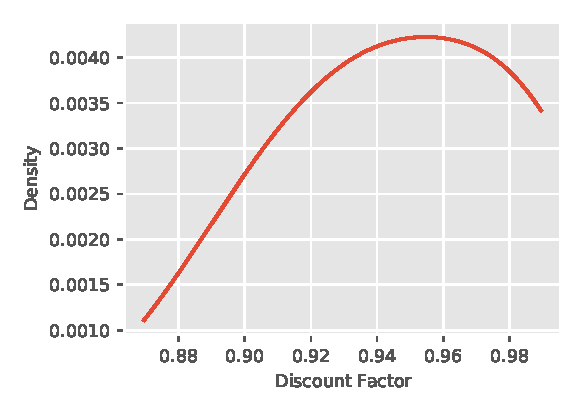
\includegraphics[width=.93\linewidth]{mainmatter/plots/SS_evaluation/Beta_density.pdf}
  \caption{Density of Discount factors.} \label{fig:Beta_dist}
\end{subfigure}%
\begin{subfigure}{.5\textwidth}
  \centering
  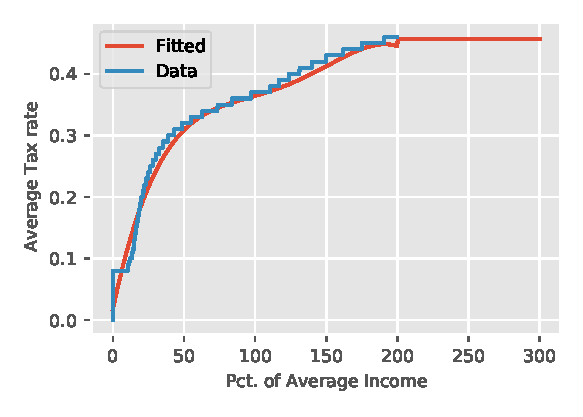
\includegraphics[width=.93\linewidth]{mainmatter/plots/SS_evaluation/tax_function1.pdf}
  \caption{Fitted tax function.} \label{fig:tax_function}
\end{subfigure}
}
\caption[Caption for LOF]{Calibrations}
\label{fig:SS_dists}
 \centering
  {\scriptsize  a) Kernel density of calibrated discount factors with average = 0.972. b) Tax function for average tax rates from the Danish Economic Council (\textit{Data}) and fit with cubic spline (\textit{Fitted}).}
\end{figure}




\bgroup
\def\arraystretch{1.0}
\setlength{\tabcolsep}{1.0em} 
\begin{table}[H]
\tiny
%\captionsetup{font=footnotesize}
\caption{Calibration} 
\label{Table:Calibration}
\centering
\footnotesize
\scalebox{0.9}{
\begin{threeparttable}
\scriptsize 
\makebox[\textwidth]{ 
\begin{tabular}{lcccc}
\toprule
\midrule
%\multicolumn{2}{c}{{Revenues}} & \multicolumn{2}{c}{Expenses} \\ 
 {Symbol}   & Desc.  & Value & Target  & Source  \\
 \cmidrule(lr){1-5}  
 
\multicolumn{5}{c}{\textbf{Households}} \\
\midrule
$\sigma$ & EIS & 0.5 & - & Standard \\ 
%$\varphi$ & Frisch Elasticity & 0.5 & - & Standard \\ 

%$\varphi$ & Disutility of labor & 0.01 & Job Finding rate = 30\% & \citet{hobijn2009job} \\ 
%$\varphi^{\ell}$ & Disutility of labor & 2.4 & $\int e_{i}\ell_{i}di=1$ & Calibrated \\ 

$\mu^\beta$ & Mean of Beta dist. & 0.93 & $r=0.5\%$ & Standard \\ 
$\Delta^\beta$ & Span of Beta dist. & 0.04 & Wealth Distribution Moments & \citet{balestra2018inequalities} \\ 
$\rho^\e$ & Persistence of earnings & 0.95 & - & \citet{floden2001idiosyncratic} \\ 
$\sigma^\e$ & SE of earnings & 0.7 & - & \citet{floden2001idiosyncratic} \\ 
$\kappa_{r^a}$ & Borrowing Wedge & $ 0.07 \cdot w_{ss}$ & 15\% of Households indebted  & \citet{kaplan2018monetary} \\ 
%\midrule
\multicolumn{5}{c}{} \\ 
\multicolumn{5}{c}{\textbf{Firms}} \\
\midrule
%$I$ & Investment rate & 0.22  & 22\% of GDP  & Statistics Denmark  \\ 
$\delta^K$ & Capital deprecation rate & 0.02  &   & Standard \\ 
%$I$ & SS Investment & 0.3  & 30\% of GDP  & Statistics Denmark  \\ 
$\kappa_P$ & Price Adj. Cost & 366  & NKPC slope = 0.03  & Standard  \\ 
$\kappa_I$ & Investment adjustment cost & 6  & -  & \citet{pedersen2013drives}  \\ 
$\kappa^V$ & Vacancy posting cost &  0.03 & $\frac{\kappa^{V}}{m}=0.07w^{ss}$ & \citet{christiano2016unemployment} \\ 
$\Phi^{F}$ & Fixed Cost &  12\% of $Y_{ss}$ & Wealth-to-Income ratio = 600\% & \citet{NB_wealth} \\ 
%\midrule
\multicolumn{5}{c}{} \\ 
\multicolumn{5}{c}{\textbf{Labor Market}} \\
\midrule
$\xi$ & Matching Elasticity & 1.4 & Unemployment rate = 5\% & Statistics Denmark \\ 
$w^{ss}$  & Steady-state wage & 0.63 &  Matching Probability = 0.7  & \citet{christiano2016unemployment} \\
$\delta^N$ & Job Destruction Rate & 0.06  & -  & \citet{hobijn2009job} \\ 
$m_t$ & Matching Probability & 0.7  & -  & \makecell{\citet{den2000job}, \\ \citet{ravenna2008vacancies} }  \\ 
$\eta_t$ & Wage elasticity  & 0.01  & -  & -  \\ 
\multicolumn{5}{c}{} \\ 
\multicolumn{5}{c}{\textbf{Government}} \\
%\multicolumn{5}{c}{} \\ 
\midrule
%$\tau^{VAT}$ & VAT & 0.25 &  -  &  Statutory Rate   \\
%$\tau^c$ & Corporate Tax rate & 0.22 &  -  &  Statutory Rate   \\
%$\tau^{div}$ & Dividend Tax rate & 0.42 &  -  &  Statutory Rate   \\
$G$  & Public Consumption & 0.24 &  24\% of GDP  & Statistics Denmark   \\
$B$  & Public Debt & 1.15 of $Y$ &  50\% of $A$  & Statistics Denmark   \\
%$\delta^{B}$  & Public Debt Maturity & 0.87 &  Maturity of 8 years  & \citet{NB_G}  \\
$b$  & Unemployment Benefits & 0.29 &  After tax Replacement rate of 51\% & \citet{schindler2011labor}  \\
$\phi^{\pi}$  & Inflation coefficient & 1.3 &  -  & Standard  \\
$\rho^{MP}$  & Interest rate smoothing & 0.8 &  -  & Standard  \\
\midrule[\heavyrulewidth]
\end{tabular}
}
\end{threeparttable}
}
%\begin{tablenotes}[para]\footnotesize 
%\item[1] The values for σ used in the literature are: 0.24 in Hall (2005a), 0.4 in Blanchard and Diamond (1989), Andolfatto
%(1994) and Merz (1995), 0.45 in Mortensen and Nagypal (2006), 0.5 in Hagedorn and Manovskii (2006), 0.5 in Farmer
%(2004), 0.72 in Shimer (2005a). See also a brief discussion in Mortensen and Nagypal (2006), p. 10, comparing their
%value of 0.45 to Shimer’s one \\
%\item[2] Labor Market Regulations in Low-, Middle- and High-Income Countries : A New Panel Database
%\end{tablenotes}
\end{table}




\subsection{Steady State Distributional Statistics}
Table \ref{table:Wealth_dist} shows how well the model fits the data in terms of the distribution of wealth. The targets (Middle 40\%, Bottom 50\%, Bottom 10\% and share of households in debt) all fit the data well, and by construction the top 10\% share of wealth also matches reasonably. The share of the top 1\% wealthiest is significantly underestimated, but this should have little implication for further analysis and is common to this type of model.0\footnote{To match the wealth share of the top wealthiest households entrepreneurial risk as in \citet{benhabib2014wealth} is usually needed.} The post-tax income Gini coefficient matches exactly the data, but given the minimal tax-transfer system the implied model pre-tax income Gini underestimates the data. 



\bgroup
\def\arraystretch{1.3}
%\setlength{\tabcolsep}{1.1em} 
\begin{table}[H] %\centering \footnotesize
\caption{Wealth Distribution - Model Fit vs. Data} \label{table:Wealth_dist}
\makebox[\textwidth]{ 
\begin{threeparttable}

\begin{tabular}{l*{2}{c}}
\hline\hline
\multicolumn{1}{c}{Share of Wealth of:}           & \multicolumn{1}{c}{Data} & \multicolumn{1}{c}{Model}    \\
%\multicolumn{1}{c}{Share of Wealth of:}           & \multicolumn{1}{c}{} & \multicolumn{1}{c}{}    \\
\hline 
Top 1\%     &  14.7\%  & 6.7\% \\  
Top 10\%    &  47.4\%  & 43.3\%  \\  
Middle 40\%   & 47.6\% & 51.7\% \\   
Bottom 50\%   & 5\% &  5\%  \\   
Bottom 10\% & -2.2\%  &  -2.4\% \\   
%Bottom 5\%  & -4.4\%  &    -4.4\% \\   
Share in debt & 15\%  & 16.4\% \\  
Share Constrained & -  & 0.9\% \\  
Wealth Gini    &  0.69 & 0.67 \\  
Income Gini (pre taxes \& transfers)   & 0.44   &   0.38  \\   
Income Gini (post taxes \& transfers)    & 0.25   & 0.31  \\   
\hline\hline 
\end{tabular}
  \begin{tablenotes}
     {\scriptsize See \citet{balestra2018inequalities} for all wealth distribution statistics. Gini coefficients for income are obtained from \citet{neamtu2014chapter}.} \\
    %\item[1] \scriptsize Negative values in the data, but given the borrowing constraint $\underline{a} = 0$ I impose that these targets must be 0. 
  \end{tablenotes}
\end{threeparttable}
}
\end{table}


Table \ref{table:Household_dist_stat} displays characteristics across the wealth and income distributions respectively. Accumulated wealth exhibits a strong, positive correlation with the degree of patience $\beta$. This in turn implies a strong correlation with marginal propensities to consume, which are strongly decreasing in wealth across the population. The last two columns in panel A shows that the income distribution is off less importance in the determination of the wealth distribution. While there is a tendency for higher skill/earnings and lower unemployment rates as one move up the wealth ladder, the correlation is not monotone. In particular, the middle part of the distribution (the 30th-50th percentile range) have higher earnings on average compared to other parts of the distribution. This implies that high earnings can bring households to the middle of the distribution, but the movement further up the wealth ladder is determined primarily by the discount factor.
Panel B of the table shows similar statistics for the income distribution. The calibration implies a positive correlation between income (skill percentile) and MPCs, but not nearly as strong as for the wealth distribution. 
In steady-state unemployed households has on average 86\% the consumption of employed households. This is significantly less than the gap between wages and unemployment benefits of $51\%$, showing the effects of consumption smoothing across states.   
%which implies that the gap between wages and unemployment benefits has more than 1-for-1 pass-through onto consumption. 


\bgroup
\def\arraystretch{1.3}
%\setlength{\tabcolsep}{.8em} 
\setlength{\tabcolsep}{1.1em} 
%\renewcommand{\arraystretch}{2}
\begin{table}[H]%[H]
%\tiny 
%\scriptsize
\footnotesize
%\begin{threeparttable}
\caption{Distributional statistics for Households} \label{table:Household_dist_stat}
\makebox[\textwidth]{ 
\begin{threeparttable}
\begin{tabular}{l  cccc}

%\toprule
%\multicolumn{5}{c}{Panel A:}  \\
\multicolumn{5}{c}{Panel A: Wealth Distribution Characteristics} \\
\cline{1-5}
\multicolumn{1}{c}{} & \multicolumn{1}{c}{{MPC}} & \multicolumn{1}{c}{{Avg. $\beta$}} 
& \multicolumn{1}{c}{{Unemployment Rate}} & \multicolumn{1}{c}{{Skill Percentile}}  \\ 
\midrule
Top 1\%     &  0.02 & 0.994 & 5.01\%  & 94.8 \\  
Top 10\%    &  0.03 & 0.991 & 5.09\%  & 94.9 \\  
70th-90th   &  0.06 & 0.981 & 4.98\%  & 94.8  \\   
50th-70th   &  0.13 & 0.968 & 4.97\%  & 83.6 \\   
30th-50th   &  0.24 & 0.955 & 4.79\%  & 83.6 \\   
10th-30th   &  0.44 & 0.945 & 4.54\%  & 69.9 \\   
Bottom 10\% &  0.69 & 0.936 & 6.37\%  & 39.9  \\   
Bottom 1\%  &  0.99 & 0.937 & 2.13\%  & 63.9 \\   
\midrule
\midrule[\heavyrulewidth]
\end{tabular}
  \begin{tablenotes}
    {\scriptsize The table shows the average MPC, discount factor, unemployment rate and skill percentile for various groups in the wealth distribution. Top 1\% refers to the 1\% holding the most assets, and similarly for Top 10\%, Bottom 10\%, Bottom 1\%. 70th-90th refers to the group between the 70th percentile in the wealth distribution and the 90th percentile, and similarly for 50th-70th, 30th-50th, and 10th-30th.   }
  \end{tablenotes}
\end{threeparttable}

}
\makebox[\textwidth]{ 
\begin{threeparttable}
\begin{tabular}{l  ccc}
%\centering
\multicolumn{4}{c}{}  \\
%\multicolumn{4}{c}{Panel B:}  \\
\multicolumn{4}{c}{Panel B: Income Distribution Characteristics} \\
\cline{1-4} 
\multicolumn{1}{c}{} & \multicolumn{1}{c}{{MPC}} & \multicolumn{1}{c}{{Avg. Income Tax rate}} 
& \multicolumn{1}{c}{{Unemployment Rate}}   \\ 
\midrule
Top 1\%     &  0.06 & 46\% & 4.5\%  \\  
Top 10\%    &  0.09 & 46\% & 4.9\% \\  
70th-90th   &  0.18 & 45\% & 4.8\% \\   
50th-70th   &  0.25 & 37\% & 4.7\% \\   
30th-50th   &  0.29 & 30\% & 5\%  \\   
10th-30th   &  0.32 & 26\% & 5.8\%   \\   
Bottom 10\% &  0.32 & 11\% & 5.1\%   \\   
Bottom 1\%  &  0.23 & 8\% & 5.3\%  \\   
\midrule
\midrule[\heavyrulewidth]
\end{tabular}
  \begin{tablenotes}
     {\scriptsize Definitions are similar to those in panel A.}
  \end{tablenotes}
\end{threeparttable}
}
%{\raggedright\footnotesize\centering {Definitions are similar to those in panel A.} \par}

%\end{threeparttable}
 
\end{table}


     % INCLUDE Discussion



\pagebreak 
\section{Consumption Analysis}
%\subsection{Calibration Review}
%\subsection{Partial Equilibrium Comparison}
Since the primary novelty of HANKs models compared with simpler NK models lie in the consumption/savings dynamics it stands to reason to review these dynamics, and discuss their empirical relevance and counterparts in other in models. First, I focus on the response of consumption to transitory shocks to income and the real interest rate, since these are the main drivers of consumption over the cycle. The second part discusses the implications for consumption responses of adding heterogeneity, and shows how a simple decomposition can split the aggregate HANK response into the response from a TANK model and a part relating to distributional dynamics. The remaining section conducts and discusses robustness w.r.t central parameters. 


%The left panel of figure \ref{fig:SS_dists} plots the estimated distribution of discount factors, while the right panel plots the marginal propensity to consume following a transitory income shock as a function of wealth. The aggregate MPC is 0.6 in period 1, which is in the middle of empirical estimates (\citet{souleles1999response}, \citet{shapiro2003consumer}, \citet{johnson2006household}, \citet{shapiro2009did}, \citet{sahm2010household}, \citet{broda2014economic}). As per the figure, the aggregate MPC is primarily driven by low wealth household, and in particular, the financially constrained who averages an MPC of 1.   \\
%Table \ref{table:Household_dist_stat} displays a number of statistics across different types of households. As also evident from the figure the MPC is largely depend on wealth, and to a much lesser extend income. 

%\subsubsection{The Marginal Propensity to Consume}
\subsection{Income shocks and Marginal Propensities to Consume}
To evaluate how well the calibrated model fit empirical consumption responses, I consider an experiment where households are subject to a transitory income shock where all households receive a lumpsum transfer corresponding to 1\% of the steady-state wage. The shock lasts only for one period, so as to match the shock carried out in \citet{auclert2018intertemporal}, since this allows for a comparison with empirical estimates of dynamic consumption responses. Figure \ref{fig:MPC_evidence_compare} plots the annual marginal propensity to consume following the shock along with the empirical estimates from \citet{fagereng2019mpc}. The authors here use lottery prizes in Norway as proxies for transitory income shocks to estimate the dynamic consumption response for households. The model fail to match the high initial MPC, but the persistence afterwards is reasonably well captured. A contemporaneous, annual MPC of 0.25 out of transitory income is not entirely consistent with the Norwegian evidence, but matches well other empirical estimates in the literature (\citet{souleles1999response}, \citet{shapiro2003consumer}, \citet{johnson2006household}, \citet{shapiro2009did}, \citet{sahm2010household}, \citet{broda2014economic} to name but a few).

The second panel (\ref{fig:MPC_wealth_SS}) plots the consumption functions for different values of $\beta$ along with the distribution of net worth. The figure partially reveals the effect of discount factors on MPCs (the slope of the consumption function), especially when taking into consideration the correlation between $\beta$ and wealth. For the most impatient the consumption function is steep, reflecting a high MPC. Since this type of household tends to be in the range with low net worth this further boosts the aggregate MPC. The slope of the consumption function for the most impatient is relatively more steep than in \citet{carroll2017distribution}, which is due to the low value of $\beta$ I obtain for these (0.913 vs 0.9867 in Carrol et. al).\footnote{Note though they assume a uniform distribution over discount factors, which I do not necessarily. The share of population on the lowest discount factors are 7\% vs. 17\% for my and Carrol et. al's calibrations respectively.  } 


%A low contemporaneous MPC is a well known weakness for the class of models in which heterogeneous-discount-factor HANK model belongs. For instance, \citet{hagedorn2019fiscal} construct a similar HANK model (minus the search-and-matching labor market) and, conditonal on calibration, obtains a quarterly MPC of 0.12 to a similar shock. For comparison, the quarterly MPC in my model is 0.19. \citet{auclert2018intertemporal} finds that a two asset HANK model a la \citet{kaplan2014model} or having bonds in the utility function as in \citet{kaplan2018microeconomic}, \citet{michaillat2018new}, \citet{hagedorn2018prices} is necessary to match the high initial MPCs. 

%The effect of bonds in the utility function is that it increases the savings stock, hence decreasing consumption for a given income. This in turn increases the marginal utility of consumption, and hence provides higher MPCs. However, since the HANK model in this paper is already calibrated to the wealth distribution in the data, this channel serves no purpose. Thus the solution would be to expand the model to contain both liquid and illiquid assets, but given the increased complexity of the model and the higher computational cost in the household's dynamic programming problem I opt to keep the more simple setup described above.  




\begin{figure}[H]
\makebox[\linewidth][c]{%
\centering
\begin{subfigure}{.5\textwidth}
  \centering
  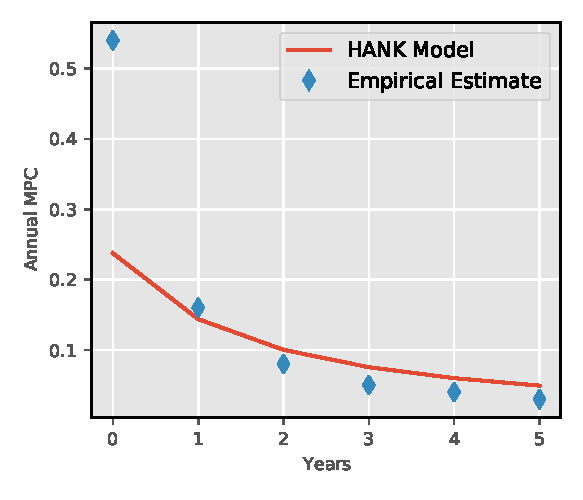
\includegraphics[width=.99\linewidth]{mainmatter/plots/SS_evaluation/Mpc_compare_Norway.pdf}
  \caption{Annual model MPCs vs. data. } \label{fig:MPC_evidence_compare}
\end{subfigure}%
\begin{subfigure}{.5\textwidth}
  \centering
  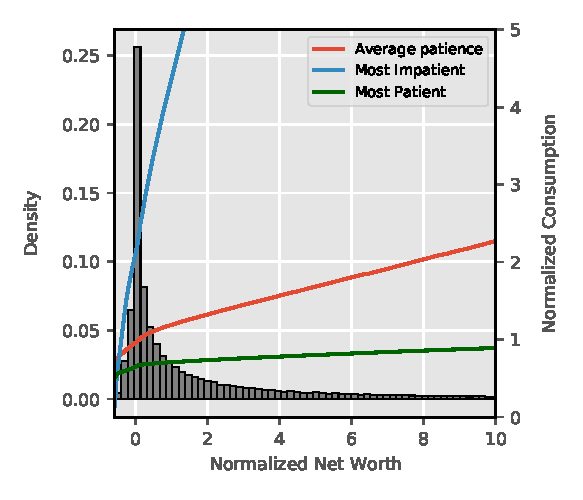
\includegraphics[width=.99\linewidth]{mainmatter/plots/SS_evaluation/Consumption_function.pdf}
  \caption{Consumption Functions and the distribution of Net worth. } \label{fig:MPC_wealth_SS}
\end{subfigure}
}
\caption[Caption for LOF]{Consumption Behavior}
\label{fig:SS_dists}
  {\scriptsize  a) Annual MPCs (calculated as $\sum_{t=0}^{3}\text{\ensuremath{\text{Quarterly MPC}_{t}}}=\sum_{t=0}^{3}\frac{dC_{t}}{dI_{t_{0}}}$) in the calibrated HANK model versus evidence from \citet{fagereng2019mpc} b) Consumption function for consumers with lowest, average and highest $\beta$ respectively and histogram of cash on hand $m_{ss}= a_{ss} + (1+\tau^{VAT}) c_{ss}$. In panel (b), all variables are normalised by income. }
\end{figure}


\subsection{Consumption and Interest rates}
I review the interest rate response for two reasons: 1) The sensitivity of consumption to interest rates vs income is obviously a key determinant in the cyclical response of consumption, 2) Determinacy. Regarding the second point recall that in the canonical NK model a sufficient condition for determinacy is that the Taylor principle is satisfied (nominal interest rate responds more than one-to-one to inflation). This applies since an increase in the real interest rate decrease consumption in the present periods thereby lowering aggregate demand and hence inflation. Since HANK models feature a generally weaker interest rate response, determinacy might not be obtained as easily.  
%This is not necessarily the case in HANK models, see for instance the results in \citet{ravn2016macroeconomic}, \citet{acharya2020understanding}. 


Figure \ref{fig:calibration_C_r} presents the response of consumption to a monetary policy loosening in the calibrated HANK model. The shock is similar to that carried out by Kaplan et. al. in \citet{kaplan2018monetary}. To contextualize the response, recall that in the RANK setup consumption follows from the Euler equation, and a drop in the interest rate hence stimulates consumption "today" through a drop in the relative price of consumption between periods. After the initial stimulus there is monotone convergence back to the steady state value of consumption. In the HANK model the relative price effect - which implies that households bring forward consumption - is present and implies an initial increase in consumption, but the effect is weaker than the corresponding RANK effect. After the initial increase consumption declines persistently relative to the steady state. 
The significantly weaker initial response stems from the calibration of discount factors. Due to precautionary savings in the HANK model a lower average discount factor is needed compared to the RANK model to match the same aggregate wealth stock.\footnote{Or equivalently, the same real interest rate.} Generally lower discount factors in the population in turn implies that households are less forward-looking, and respond less to changes in the interest rate through intertemporal substitution. Note though that the presence of uncertainty about the future implies an opposite effect since households prefer to consume today with certainty rather than postpone consumption to the uncertain future. 

Regarding the persistent decline afterwards, note that when the interest rate declines the net worth of the household declines due to lesser interest on existing assets, i.e. lower financial income. Since households respond more aggressively to changes in income and net worth in the heterogeneous agent setup there is a large negative effect on consumption from this channel. This is unlike the RANK setup and also not in line with the impulses from the two-asset model of Kaplan et. al. where aggregate consumption declines only marginally after the initial stimulus.   

What are the differences between the two HANK models that imply so wildly different consumption responses? The model of Kaplan et. al. features two assets, one liquid and one illiquid. Their calibration implies that aggregate household wealth is composed of 10\% liquid assets and the remaining 90\% is illiquid assets. Thus, a shock to interest rate on liquid assets affect only a small part of overall households wealth, whereas in the one asset HANK model it affects the entirety of wealth. Since the effect of the interest rate on net worth is proportional to the relevant asset stock the effect on net worth is significantly smaller in two-asset setup.\footnote{Given the budget constraint $m_{t}=I_{t}+(1+r_{t})a_{t-1}$ where $m_{t}=c_{t}+a_{t}$ measures net worth, the mechanical effect of a change in the interest on net worth is $\frac{dm_{t}}{dr_{t}}=a_{t-1}$.}


%This is closely related to the concept of “unhedged interest rate exposure” (URE) from \citet{auclert2019monetary} 

%More formally, \citet{auclert2019monetary} shows (theorem 3) that the partial equilibrium response of consumption to a change in the interest rate with no persistence is given by:
%\begin{gather*}
%dC_{t}=\left(\underbrace{\operatorname{Cov}\left(MPC_{i},URE_{i}\right)}_{\text{Interest rate exposure channel %}}-\sigma\underbrace{E\left[\left(1-MPC_{i}\right)c_{i}\right]}_{\text{Substitution channel }}\right)\frac{dR}{R},
%\end{gather*}
%where $URE_{i}$ - the \textit{unhedged interest rate exposure} of household $i$ - is given by %$URE_{i,t}=\left(1-\tau_{i,t}^{I}\right)I_{i,t}+a_{i,t-1}-\left(1+\tau^{VAT}\right)c_{i,t}$ and equals the difference between all maturing assets and %liabilities. The covariance and expectaional terms are taken over the cross-sectional distribution. 


%Regarding empirical estimates, macroeconometric analyses of time-series data (\citet{campbell1989consumption}, \citet{yogo2004estimating}) finds that consumption is relatively insensitive to changes in the interest rate when controlling for income. This is not consistent with standard RANK models under realistic parameterizations of the EIS. Recent micro data evidence in \citet{holm2020transmission} finds that the consumption response to changes in the interest rate is - unsurprisingly perhaps - very heterogeneous across the wealth distribution. The authors finds that households at the bottom of the wealth distribution simply increase consumption in response to a monetary loosening while households in the middle of the wealth distribution decrease savings. For households at the top of distribution, their response is primarily determined by changes in financial income since they hold large amounts of assets. In particular, these households initially decrease both consumption and savings, hence showing less RA-like behavior. Foreshadowing the next section, the robustness analysis in \ref{sec:C_robustness} shows that the HANK model has some issues replicating these heterogeneous effects. For instance, because households at the top of wealth distribution also tend to have a high degree of patience, they increase consumption significantly initially (forward substitution through the Euler equation), while the financial income channel pointed out by Holm et. al. only enters in later periods, albeit relatively strongly. They also find that the effect through financial income should affect households at the bottom of the distribution strongly, though this is not something I find since these households tend to be impatient.\footnote{I conjecture that the financial income channel is weak for poor households due to the limited modeling of indebted households (tighter borrowing constraints than standard calibrations + no interest rate differential). }  

Regarding empirical estimates, macroeconometric analyses of time-series data (\citet{campbell1989consumption}, \citet{yogo2004estimating}) finds that consumption is relatively insensitive to changes in the interest rate when controlling for income. This is not consistent with standard RANK models under realistic parameterizations of the EIS. Recent micro data evidence in \citet{holm2020transmission} finds that the consumption response to changes in the interest rate is - unsurprisingly perhaps - very heterogeneous across the wealth distribution. The authors finds that households at the bottom of the wealth distribution simply increase consumption in response to a monetary loosening while households in the middle of the wealth distribution decrease savings. For households at the top of distribution, their response is primarily determined by changes in financial income since they hold large amounts of assets. In particular, these households initially decrease both consumption and savings, hence showing less RA-like behavior. Foreshadowing the next section, the robustness analysis in \ref{sec:C_robustness} shows that the HANK model has some issues replicating these heterogeneous effects. For instance, because households at the top of wealth distribution also tend to have a high degree of patience, they increase consumption significantly initially (forward substitution through the Euler equation), while the financial income channel pointed out by Holm et. al. only enters in later periods, albeit relatively strongly. They also find that the effect through financial income should affect households at the bottom of the distribution strongly, though this is not something I find since these households tend to be impatient.

% How does this relate to my HANK model?


% covariance is negative: 

%When disposable income begins to fall in response to a monetary policy contraction, households
%with low liquid asset holdings let their consumption decline, while households with intermediate
%amounts of liquid assets initially reduce saving or increase borrowing, as predicted by theory.

% n contrast, we
%find that households with large liquidity positions increase both consumption and saving after
%a monetary tightening, before consumption ultimately falls

\begin{figure}[H]
\makebox[\linewidth][c]{%
\centering
  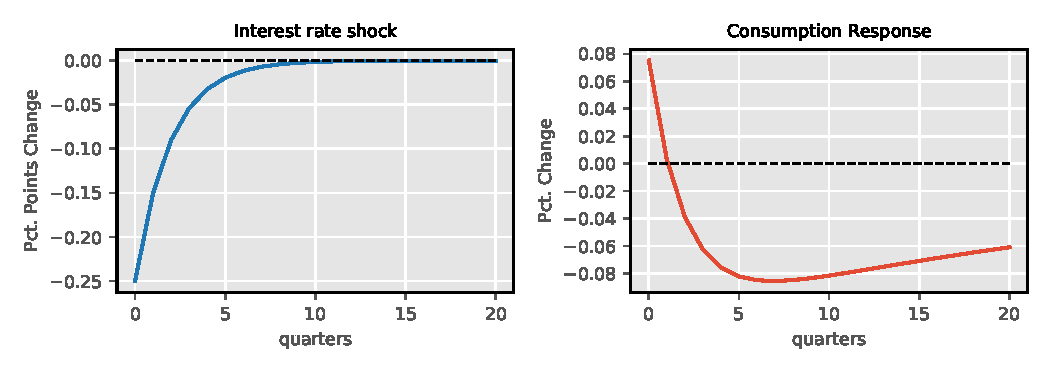
\includegraphics[width=.98\linewidth]{mainmatter/plots/SS_evaluation/Consumption_interest_rate_response.pdf} 
}
\caption{Impulses to a temporary interest rate shock analogues to \citet{kaplan2018monetary}.}
\label{fig:calibration_C_r}
    \scriptsize
    \centering
    {
    \emph{Note:} Response to a -0.25 percentage point drop in the real interest rate with persistence 0.6. }
 % {\scriptsize  Impulse responses to a negative productivity shock of 1\% with persistence 0.94 (half-life: 5 quarters). }
\end{figure}


\subsubsection{Liquid vs. Illiquid assets.} As an example of this compositional effect arising in the KV two-asset model, consider the following example: Imagine that assets $a_{i,t}$ is composed of 10\% liquid assets which yields return $r$ set by the central bank, and 90\% percent illiquid assets $\bar{a}_i$ which yields exogenous return $\bar{r}$, which equals the steady state return. Assume further that the Euler equation uses the rate $r$. Figure \ref{fig:dC_dR_illiquid_example} in the appendix shows consumption responses under this calibration. The response moves closer to the RA response, and closely resembles that from Kaplan et. al. Note though, that in the KV-model changes in the monetary policy rate also affects the return to illiquid assets and hence also generates changes to financial income. This, however, occurs only in the general equilibrium where the monetary policy rate affects the return to capital and firm equity. 

%no-arbitrage conditions between the return to liquid and illiquid assets imply that the return to illiquid assets are directly affected by interest rate changes. The crucial mechanism w.r.t the consumption response is that the presence of adjustment costs for illiquid assets ensures that this stock adjusts only slowly to 



These considerations tie directly into the discussion of whether the calibration of single asset macroeconomic models should reflect overall net worth or only liquid assets, see in particular \citet{carroll2017distribution}. Carrol et. al. show that their "Beta-dist" model - which closely resembles the household model in this paper - matches empirical MPCs well, and does so in a simpler setting than the KV two-asset model. However, as shown here the weakness of the "beta-dist" model is that it generates a relatively volatile consumption response to a real interest rate shock. The KV model, and by extension the two-asset HANK model, excels in this regard. 


\subsubsection{Borrowing} Note that allowing for borrowing (i.e. allowing $a_{i,t}<0$) aids the one-asset HANK model in replicating the interest rate response of the KV HANK model since a monetary policy loosening implies a decrease in interest payments on debt and hence an increase in income for indebted households.  However, allowing for borrowing up to usual amounts (one quarterly wage rate for unsecured borrowing, which borrowing is to be interpreted under my calibration) gives rise to an unrealistic wealth distribution where large parts of the population is indebted if there is no interest rate differential. 
%Allowing for different interest rates to debtors and creditors creates a borrowing wedge, which replicates realistic wealth distributions by generating large masses of household around the zero net-worth cutoff. The solution to the households problem is however complicated since there is a kink in the budget constraint at $a_{i,t} = 0$. As a consequence a more general EGM method, as discussed in \citet{druedahl2019guide}, must be applied. For this reason I calibrate the borrowing limit to match share of households in debt, with the resulting limit being less than the quarterly wage rate-limit usually assumed.   
%However, for realistic borrowing limits - usually considered to be one quarterly wage rate for unsecured borrowing - this mechanism is not sufficiently large to alleviate the issue.  
%This is of course a direct application of the unhedged interest exposure channel discussed above.

% Unheged interest exposure 
%\subsubsection{Debt Maturity.} Obviously the simplistic structure of households balance sheets matter for the interest rate response. As is common in simple NK models all assets of the household mature every period, and hence changes in the interest rate has full pass-through onto financial income. A more complete modeling of household balance sheets and asset compositions where maturity is not immediate will also provide more realistic responses. Debt maturity can be easily implemented in the governments supply of bonds (see \citet{auclert2020micro}), but it is less obvious to implement in firm equity since dividends are generated each period.  







\subsection{Dynamic Consumption Responses - Discount Factor Heterogeneity} \label{sec:C_robustness_disc}
To better explain consumption and welfare changes across households Figure \ref{fig:calibration_C_r_beta} considers the average consumption responses for each of the different discount factor groups in the baseline model. Through a close correlation with the wealth distribution (recall table \ref{table:Wealth_dist}), the model displays a wide amount of heterogeneity in responses by discount factors. For the income shock the contemporaneous (annual) MPC varies from 0.05 to roughly 0.6 with the min/max MPCs being represented by the lowest and highest discount factor groups respectively. Furthermore, the persistence of the income shock declines monotonously in discount factors. To this end, recal that in the  limiting case where households act as HtM agents exhibit zero persistence.    

For the interest rate shock the responses are also prone to heterogeneity. For patient households the on-impact effect of a lower interest rate is relatively low, and almost negative for the most patient households. The reason, as argued earlier, is that the drop in financial income generates a persistent consumption drop, and even though a drop in the relative price of consumption implies more consumption today the high marginal utility in the future due to lower income implies that consumption today must be cut. For impatient households, who hold less wealth, the financial income channel is weak and their response more closely resemble that of a representative agent where the on-impact effect is governed primarily by the drop in the relative price of consumption. Note also that for impatient households a larger share of households tend to be indebted and a drop in the interest rate hence reduces interest payments thus increasing consumption.  


%though this tendency is not strict. From the 2nd quarter and onwards consumption declines, with the decline being monotone in discount factors. This stems from the correlation between $\beta$ and wealth: The effect of a change in the interest rate in the budget constraint is $a_{i,t-1}dR_{t}$ and is hence proportional to the level of wealth, and patient households who have accumulated high levels of wealth are hence subject to large drops in financial income compared to less patient households. 


% ADD LIQUID VS ILLIQUID WEALTH SECTION 

\begin{figure}[H]
\centering
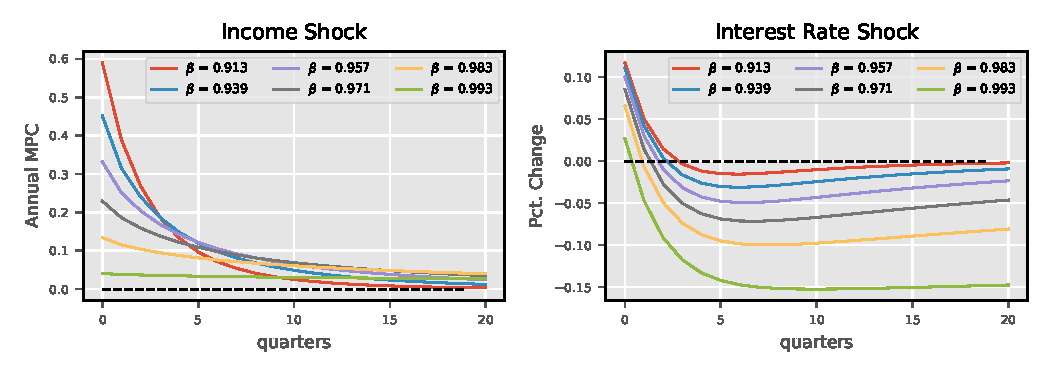
\includegraphics[width=.98\linewidth]{mainmatter/plots/SS_evaluation/Alternative_calibs/beta_dR_dI.pdf} 
\caption{Consumption responses to income and interest rate shocks by discount factor.}
\label{fig:calibration_C_r_beta}
\end{figure}


The appendix, section \ref{sec:C_robustness}, considers the consumption responses by different values of the standard deviation of earnings and the intertemporal elasticity of substitution, conditional on the wealth distribution. The standard deviation matters little when calibration to the wealth distribution, but the value of the intertemporal elasticity matters greatly. 



\subsection{Timing} 
As I analyze a persistent shock to the interest rate it involves both static effects as well as forward looking, exceptional effects. The static effect occurs in period 0 and involves no forward-looking behavior as the shock is unexpected, and consists only of a drop in financial income occurring through a lower interest rate. The forward-looking channel occurs both directly through changes to the future interest rate (since the shock is persistent, and the interest rate appearing in the Euler equations is that of the next period) as well as through changes to future marginal utilities of consumption. The second channel can potentially be strong in the general equilibrium, weak but persistent shock can be propagated since households precautionarily cut consumption today in expectation of having to smooth consumption over the duration of the shock.
I note once again that this is still a partial equilibrium setting, so even though the job-finding rate changes employment and wages stays constant. 
 

\begin{figure}[H]
\centering
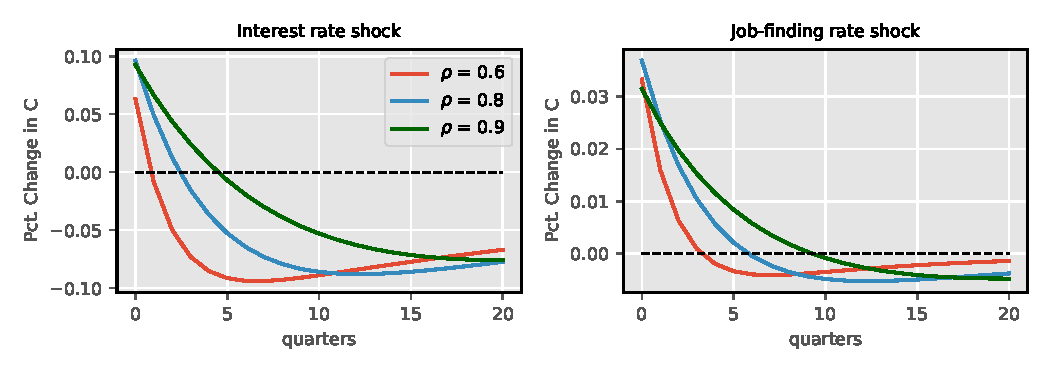
\includegraphics[width=.98\linewidth]{mainmatter/plots/C_analysis/ra_q_shocks_C.pdf} 
\label{fig:C_analysis_q_r}
\caption{Consumption responses to interest- and job-finding rate shocks with differing persistent.}
    \scriptsize
    \centering
    {
    \emph{Note:} Each panel plots the consumption response to a shock to either the real interest rate or the job-finding rate. The baseline shocks have $\rho=0.6$ with the -on-impact drop being 0.25 pct. points and 5\% for the two shocks respectively. The shocks with $\rho=0.8,0.9$ have been re-scaled such that the cumulative shock are the same across the shocks.   }
\end{figure} 

As the latter part of the thesis investigates persistent labor market dynamics, I here foreshadow this a bit in investing the effect of more persistent shocks to the job-finding rate. Figure \ref{fig:ra_q_shocks} in the appendix plots the shocks, Figure \ref{fig:C_analysis_q_r} plots the consumption responses. In interpreting the shocks there are two things to note. Since the Euler equations are forward looking in interest rates an unexpected change affects contemporaneous consumption only through changes in financial income, not intertemporal substitution. Similarly an unexpected change in the job-finding rate has no affect on consumption in period 0 \textit{when keeping employment fixed}, again due to the forward-looking nature of the Euler equations. Hence precautionary motives from unemployment risk are only induced when shocks to the finding rate are persistent and expected. 

The figure shows for both shocks that even though the most persistent shock is roughly 5 times as small on impact the effect on contemporaneous consumption is roughly the same across the shocks. Additionally and unsurprisingly, the more persistent shocks also generates more long-lived responses.  
As a side note, the shock to the job-finding rate shows that a persistent increase in-job finding rates increases only consumption by a marginal 0.03\%, with an on impact elasticity of $0.006$ for the least persistent shock. The most persistent shock has an elasticity of $0.03$.



%\subsubsection{Behavioral and distributional effects}
\subsection{Representative-Heterogeneous Agent Equivalence} \label{sec:Aggre_result} %  - An Aggregation Result
\subsubsection{Canonical Household models.} In the above discussion, I make numerous references to the canonical representative (or Ricardian) agent household structure, and the two agent model of \citet{campbell1989consumption}. The representative agent model is characterized by complete markets. The presence of these markets imply that households can perfectly insure against idiosyncratic and labor market risk, and essentially all risk that does not affect households equally.\footnote{More formally the assumption of complete markets assume the existence and availability of a complete set of Arrow-Debreu state contingency claims such that households can insure against every possible state. Trading these claims amongst themselves imply that all households obtain the same marginal utility of consumption, and are hence symmetric.} Appendix \ref{sec:RA_TA} contains the details, but optimization implies that consumption obeys the Euler equation:
\begin{gather*}
\left(C_{t}^{R}\right)^{-\frac{1}{\sigma}}=R_{t+1}\beta\left(C_{t+1}^{R}\right)^{-\frac{1}{\sigma}}
\end{gather*}
where $C^R$ denotes consumption of the representative/Ricardian/Rational agent. This results in a permanent-income setup where transitory income shocks have only marginal effects on current consumption. To counter this empirical oddity, \citet{campbell1989consumption} added Hand-to-Mouth households to the model, the resulting model being the two-agent (TA) model. HtM households holds no savings and consume their entire income each period, with resulting MPC equal to 1. Let $\lambda$ denote the share of HtM household. Consumption of these household is: 
\begin{gather*}
C_{t}^{HtM}=\left(\lambda I_{t}-\tau\left(\lambda I_{t}\right)+\lambda T_{t}\right),
\end{gather*}
with resulting aggregate consumption $C_{t}=C_{t}^{R}+C_{t}^{HtM}$. The share of HtM households $\lambda$ allows the model to capture two extreme states: For $\lambda=0$ shocks are very persistent since Ricardian households smooth consumption extensively, but MPCs are only marginal. For $\lambda=0$ the aggregate MPC is equal to 1 but shocks have no persistence. 
% proof \ref{Agg_result_proof}

% WTIHIN VS BETWEEN EFFECTS
% HANK = BETWEEN
% RANK/TANK = WITHIN 

%Keeping the distribution fixed imply that households are either always constraint or always obeying the Euler equation, and do not shift endogenously between these two states. This in turn that implies that   

\subsubsection{An Aggregation Result.} I now briefly compare the HA-household responses to the RA/TA-household responses in a partial equilibrium. Suppressing dependencies of the consumption function $c_{t}^{*}\left(a_{i,t},e_{i,t},\beta_{i},k_{i,t}\right)$ aggregate consumption is given by $C_{t}=\int c_{t}^{*}d\mathcal{D}_{t}$. A first-order perturbation around the steady-state yields: 
\begin{gather*}
dC_{t}= \underbrace{\int dc_{t}^{*}d\mathcal{D}_{ss} }_{\text{Static Effect}} + \underbrace{\int c_{ss}^{*}d\mathcal{D}_{t}}_{\text{Distributional Effect}} 
\end{gather*}
The firm term, which I dub the "static effect", captures how individual consumption changes \textit{conditional on placement in the earnings and asset distribution.} Since the placement in the ergodic distribution is determined by the dynamics of the budget constraint, the static effect - which holds constant this channel - corresponds to the dynamics of the RA (if no households are constrained in the steady-state) and TA models (if there exists constrained households in the steady-state): For rational, forward looking agents the Euler equation governs all dynamic responses, and for hand-to-mouth agents the budget constraint contains by definition no dynamics. Hence the difference between RA/TA and HA models in the partial equilibrium can be captured by the term $\int c_{ss}^{*}d\mathcal{D}_{t}$ to the first-order. Alternatively, the "static effect" term can be interpreted as a within-group effect and the "distributional effect" term a between-group effect. Appendix \ref{Agg_result_proof} contains a formal proof that the static effect term aggregates to a RA/TA setup.
%, keeping wages fixed.\footnote{Fixing wages imply no endogenous change in labor supply. This simplifies aggregation since otherwise an interaction between labor supply and heterogeneous earnings occur. } 

Figure \ref{fig:C_decomp_over_dist} shows this decomposition for the income and interest rate shock discussed in detail earlier. Perhaps unsurprisingly, but nonetheless interesting, it shows that changes in the income and wealth distribution of households accounts for the majority of persistence in the partial equilibrium impulses. For the income shock the persistence is generated by the fact that the model features low-wealth households who simultaneously have high MPCs and are forward looking. For the interest rate shock persistence is generated by a transitory drop in financial income. 


\begin{figure}[H]
\makebox[\linewidth][c]{%
\centering
  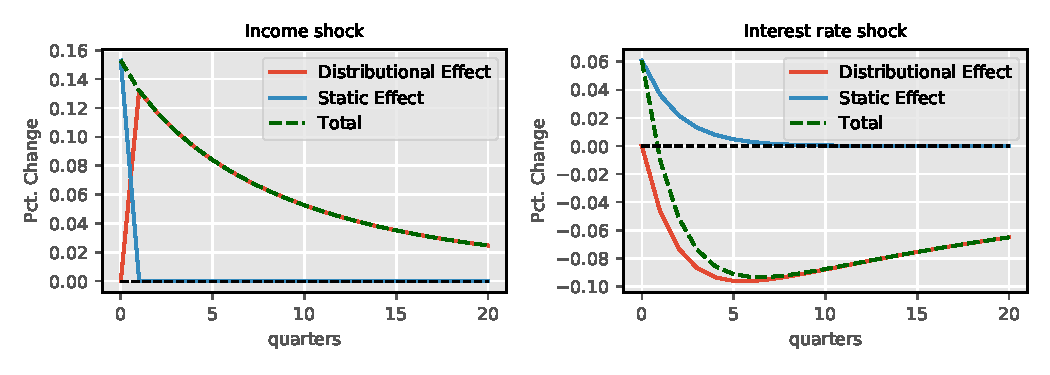
\includegraphics[width=.98\linewidth]{mainmatter/plots/C_analysis/dC__decomp_dist.pdf} 
}
\caption{HA responses decomposed in static and distributional effects. }
\label{fig:C_decomp_over_dist}
%\centering
 \scriptsize  
 \emph{Note:} The Static effect $\int dc_{t}^{*}d\mathcal{D}_{ss}$ in response to a shock keeps constant the distribution of households across states, while the distributional effect $\int c_{ss}^{*}d\mathcal{D}_{t}$ keeps constant consumption decisions. To a first-order approximation the total effect is the sum of the two effects. 
\end{figure}

\begin{figure}[h]
\makebox[\linewidth][c]{%
\centering
  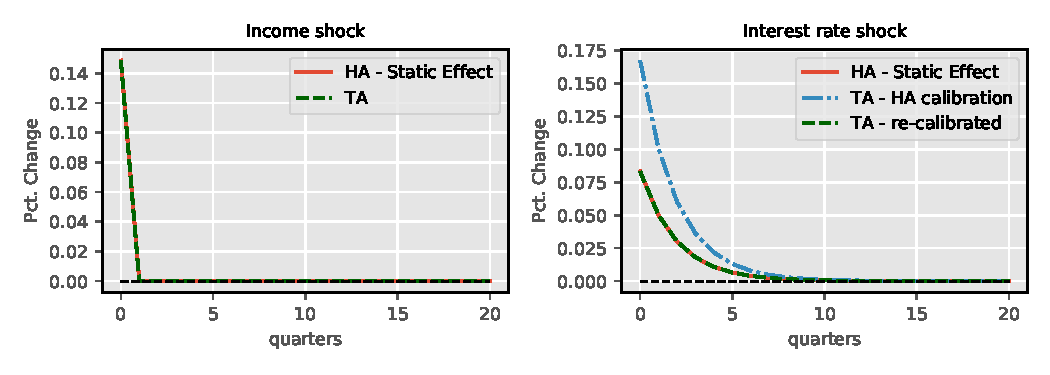
\includegraphics[width=.98\linewidth]{mainmatter/plots/C_analysis/TANK_vs_HANK_behavoiral_decomp.pdf} 
}
\caption{static from HA vs. TA responses.}
\label{fig:HANK_vs_TANK}
    \scriptsize
    {
    \emph{Note:} Each panel plots the static response $\int dc_{t}^{*}d\mathcal{D}_{ss}$ from the HA model against a calibrated TA. The TA model's share of HtM consumers is calibrated to match the initial MPC of the HA model. The 'TA - HA calibration' model refers to a TA-model with the interest rate from the HA model, while 'TA - re-calibrated' re-calibrates the interest rate and discount factor to match the initial response of consumption to an interest rate shock in the HA model.}
\end{figure}

Figure \ref{fig:HANK_vs_TANK} shows the extent of the equivalence. The left panel plots the static effect from the HA model $\int dc_{t}^{*}d\mathcal{D}_{ss}$ against a standard TANK model for the income shock, with the share of HtM consumers in the TA model calibrated to match the initial MPC of the HA model.\footnote{The RA/TA models are described in appendix \ref{sec:RA_TA}.} The two responses intersect exactly. \\
The right side panel conducts a similar exercise for the interest rate shock. However, here calibration matters to a larger extend. Applying the same interest rate as in the HANK model implies a discount factor of $\beta^{TA}=\frac{1}{1+r_{ss}^{HA}}-1$ in the TA model. Due to precautionary savings, this RA discount factor is significantly higher than the average discount factor in the HA model. This explains the majority of the difference between the HA and TA (HA calibration) responses in the panel. To this end, I re-calibrate the real interest rate in the TA model (and hence the discount factor) to match the initial response of the HA model. Again, the two curves intersect exactly. Thus the HA model contains the TA model as a special case where the term ${\int c_{ss}^{*}d\mathcal{D}_{t}}$ is held constant, \textit{conditional on calibration}.





\begin{figure}[h]
\makebox[\linewidth][c]{%
\centering
  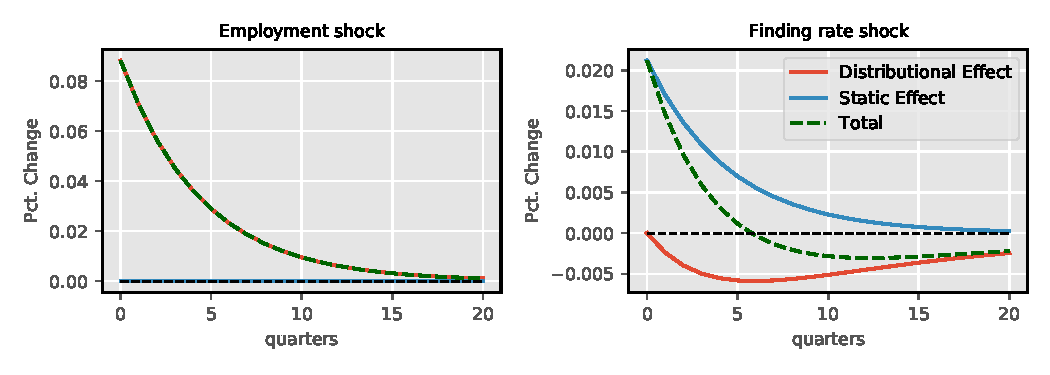
\includegraphics[width=.98\linewidth]{mainmatter/plots/C_analysis/dC__decomp_dist_N_q.pdf} 
}
\caption{HANK responses decomposed in static and distributional effects for a positive employment and job finding rate shock respectively. }
\label{fig:C_decomp_over_dist_N_q}
\centering
    \scriptsize
    {
    \emph{Note:} Each panel decomposes the total response to a shock in a distributional and a static response. The left panel considers a 1\% increase in employment with persistence 0.8, and the right panel considers a positive job-finding rate shock with the same proprieties.}
\end{figure}

\subsubsection{Employment and job-finding rates.}  Figure \ref{fig:HANK_vs_TANK} shows the distributional/static decomposition for a positive employment shock and a positive job-finding rate shock. The employment shock consists only of the distributional effect of shifting households from an unemployed state to an employed state since I keep the job-finding rate constant. The shock, however still delivers a more persist response than the underlying shock due to wealth accumulation. For the job-finding rate shock the static effect through the Euler equation dominates the total response, 
Note that the contemporaneous effect on consumption from higher employment equals exactly the average difference between consumption of employed and unemployed households in steady-state. \footnote{$dC_{t}=C_{ss}^{k=N}N_{t}-C_{ss}^{k=U}N_{t}\Leftrightarrow\frac{dC_{t}}{C_{ss}}=\frac{C_{ss}^{k=N}-C_{ss}^{k=U}}{C_{ss}}N_{t}$.} Due to households self-insuring against unemployment risk this consumption wedge is significantly less than the replacement ratio of 51\% (roughly 14\%), and the impact of employment changes is lessened. 


%\subsubsection{Heterogeneity, wealth accumulation and persistence.} Figure \ref{fig:HANK_vs_TANK} reveals that one significant dimension which the HA-model contributes to is persistence. Because shocks to income and interest rates move households around in the wealth distribution, and this in turn affect future consumption/savings decisions, these shocks have long lasting effect compared to the RA/TA-counterparts. To further exemplify this channel, consider figure \ref{fig:C_decomp_over_dist_N_q}, which decomposes the HA response to a positive employment shock and a positive job finding rate shock 
%\footnote{While the "behavioral" effect of the HA model has a direct equivalence to the TA household model when considering income and interest rate shocks, this is not necessarily the case for the job finding rate shock. If the TA household model derives from a  representative family construct, complete insurance imply changes in the finding rate has no affect on consumption, holding employment fixed. To obtain responses comparable with the HA model one needs to assume uninsurable unemployment risk.} 


%For instance, for the employment shock the behavioral effect (RA/TA-effect) has faded out after 20 quarters, whereas the distributional effect is still well above the steady-state level. 




%\subsection{Reflection} % Job finding rate response. 
%I have so far considered how consumption reacts to changes in disposable income and interest rates, which are the two primarily channels that may affect consumption. Consider for a moment how each of these channels are affected by the business cycle. 

% C makes up roughly half of Y in DK 
% more volatile than GDP, but 1/3 as volatile as I. However I share of Y is 16%. 


%In typical NK models changes in disposable income are generated by changes in wages, employment, lump sum transfers and, potentially, dividends. Wages are usually considered very rigid, almost acyclical, and dividends are modeled as firm equity, not transfers. Hence it is mostly employment and lump sum transfers that can move disposable income and hence consumption. As per the exposition above, interest rates affect consumption, but probably not enough to account for the aggregate volatility observed. What remains to affect consumption decisions is essentially precautionary savings, i.e. the fact that households increase savings by cutting consumption when faced with an increase in risk. In the present model the only source of cyclical risk is through the labor market job-finding rates. 


%The remaining channel affecting consumption is not related to income or financial flows but rather behavior and expectations. In
% Add section analyzing finding rates? 


\subsection{General Equilibrium Transmission of a TFP Shock}


%\subsubsection{Baseline Impulse Responses}
% Size of shock? 
%This section briefly dissects a negative investment shock in the baseline model (a shock to $Z^I_t$). I will use this type of shock as the main source of exogenous variation in the model, partly because it is the main driver of business cycles according to some (\citet{justiniano2010investment}), but also because this type of shock can generate labor and capital responses with same sign, which is not necessarily the case with a TFP shock. This simplifies the analysis. 
%also Corona crisis 

\subsubsection{Baseline Impulse Responses.}
I now move to the general equilibrium model described in detail in section \ref{chap:Model1}. For this purpose, I subject the model to an unanticipated, 1\% negative productivity shock with persistence 0.8. Since impulse responses are obtained through first-order approximations the responses are symmetric to the sign of the shock, and all considerations apply equally to a positive shock. Figure \ref{fig:baseline_impulse} shows the results. 
%In this experiment the government adjusts only bonds taxes to satisfy its budget constraint. Under different circumstances, this would accompanied by a tax reaction function which ensures that public debt does not explode, but given the shape of the shock and stability of the remaining model blocks, government debt converges back to the steady-state level even without changes in taxation. Thus I simplify the analysis by simply omitting the tax reaction function.  

The unexpected decrease in productivity increases the real marginal costs of firms, and hence prices. However, due to Keynesian frictions (nominal rigidities) prices only take some of the adjustment, and employment and investment hence decline due to lower marginal products. Lower employment and wages implies a drop in aggregate demand. Furthermore, consumption also declines for precautionary reasons as the job-finding rate drop. The central bank responds to the increase in inflation by increasing the real interest rate through the nominal rate. This is consistent with empirical evidence for neutral technology shocks, see for instance \citet{christiano2016unemployment}. 
%, leading to a partial stabilizing of demand in the contemporaneous period, but prolonging the negative effects of the shock.\footnote{Note that investments tends to overshoot in response to a negative shock. This comes from particular functional form of investment adjustment costs.} 

The middle panel of the figure displays the response asset variables (Households assets $A$, government bonds $B$ and firm equity $p^e$). In response to the negative shock government revenue from income and consumption taxes decline and expenses to unemployment benefits increases, 
and to maintain budget balance more bonds are issued. 
%To avoid explosive debt dynamics this turn forces the government to cut transfers to households, albeit with a lag.  
For firms the economic downturn imply a decrease in profits and dividends. Since firm equity equals the discounted stream of future dividends the value of firm shares drop. Overall, household's stock of wealth increases from period 1 and onwards. Compared to models which features only firm equity and/or capital as assets Keynes' paradox of thrift is partially alleviated here since the government issues debt over the cycle to fill the gap from lower tax revenue, thus acting as a buffer for household savings. In models with only capital/firm equity the paradox of thrift implies that household savings increase in the partial equilibrium for precautionary reasons but decrease in the general equilibrium since the drop consumption decreases demand and hence firm profits/dividends and capital, leading to a drop in the aggregate stock of assets. 


%\footnote{Simple NK models usually contain counter-cyclical markups such that profits/dividends increase in response to negative shocks. This is also the case in present model. }


%Since obviously the asset market is an important determinant of the dynamic response of the model, I will also discuss this a bit. The market equilibrium condition states that $A=B p^G + p^e$, i.e. household wealth equals the sum of government bonds and firm equity. Each component in this balance is affected wildly different by the shock. 
%For household wealth there are opposing forces: Aggregate income drops, and the real interest declines - this speaks to a decline in assets. However, as the job finding rate declines households increase savings for precautionary reasons, which speaks to an increase. 

%I consider a relatively persistent shock to technology since otherwise the initial positive effect on employment dominates, and the adverse effects from declining job finding rates are non-existent. The fact that an adverse technology shock initially stimulates employment (and vice-versa for a positive shock) is common in medium scale DSGE models - see for instance the impulses in \citet{pedersen2013drives}, \citet{christiano2016unemployment} etc. 

Overall, the shock is consistent with magnitudes in \citet{gornemann2016doves}, though the shock presented here contains significantly more persistence, mainly due to the dynamics of public debt, something which is entirely left out in \citet{gornemann2016doves}.\footnote{Gornemann et al. assumes no public debt, and that a proportional tax on labor income is adjusted at every instant to finance unemployment benefits.}

%The employment response (and consequently the job-finding rate) is rather volatile, though this is not totally unwarranted. \citet{christiano2016unemployment} estimates a peak response of output of 0.4\% following a one standard deviation TFP shock. The response of employment is 0.1\% and for the job-finding rate 1\%. The implied elasticities w.r.t output are 0.25 and 2.5 respectively. The comparable elasticities in my model are 0.94 and 5.   

%Note though that there model features utilization. This implies that labor and capital quantities need to move less to obtain a given output response. 

\begin{figure}[H]
\makebox[\linewidth][c]{%
\centering
  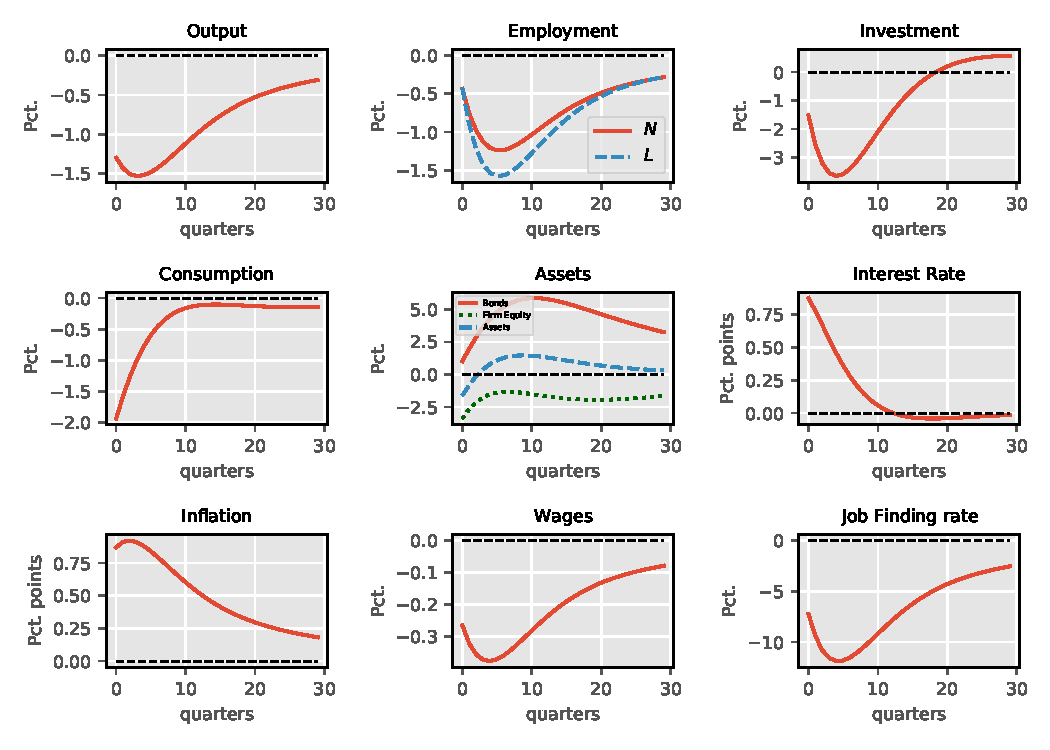
\includegraphics[width=.98\linewidth]{mainmatter/plots/SS_evaluation/main_shock.pdf} 
}
\caption[Caption for LOF]{Impulse responses to a negative productivity shock.}
\label{fig:baseline_impulse}
\scriptsize
\centering
\emph{Note:} Impulse responses to a negative productivity shock of 1\% with persistence 0.8. 
\end{figure}

%\begin{figure}[H]
%\makebox[\linewidth][c]{%
%\centering
%  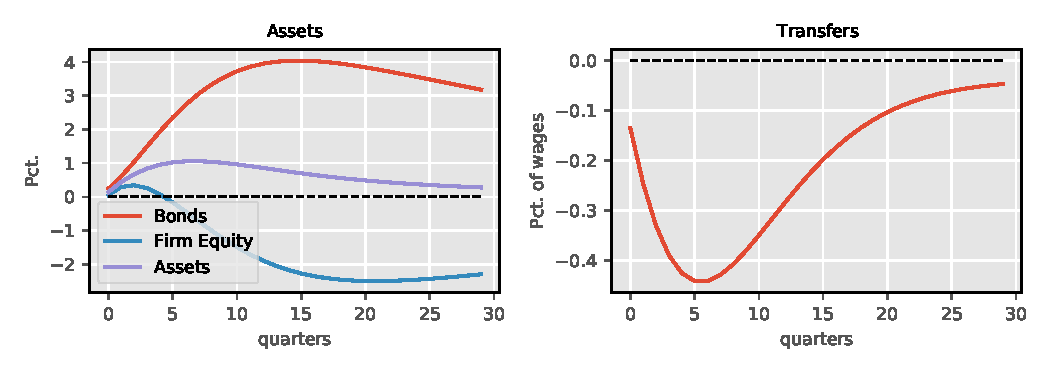
\includegraphics[width=.98\linewidth]{mainmatter/plots/SS_evaluation/Assets_transfers.pdf} 
%}
%\caption[Caption for LOF]{Responses of assets and transfers.}
%\label{fig:baseline_impulse_assets_transfers}
% % {\scriptsize  Impulse responses to a negative productivity shock of 1\% with persistence 0.8. }
%\end{figure}
\subsubsection{Decomposing Aggregate Consumption.}
Aggregate consumption $C_{t}$ is a function of paths $\left\{w_{t},r_{t},q_{t},N_{t}\right\} _{t\geq0}$, and given a particular general equilibrium path $\left\{ x_{t}\right\} _{t\geq0}\in\left\{w_{t},r_{t},q_{t},N_{t}\right\} _{t\geq0}$ the effect of this particular $x$ on $C$ can be obtained by a first-order approximation. Figure \ref{fig:baseline_C_decomp} shows the resulting decomposition. Half of the initial drop is caused by higher interest rates, while increased unemployment risk through lower job-finding rates account for 1/3 of the drop. Lower wages and higher unemployment account for the remaining drop. The majority of the consumption response can be said to be driven by the interest rate, though the job-finding rates has a non-trivial effect too. 

\begin{figure}[H]
\makebox[\linewidth][c]{%
\centering
  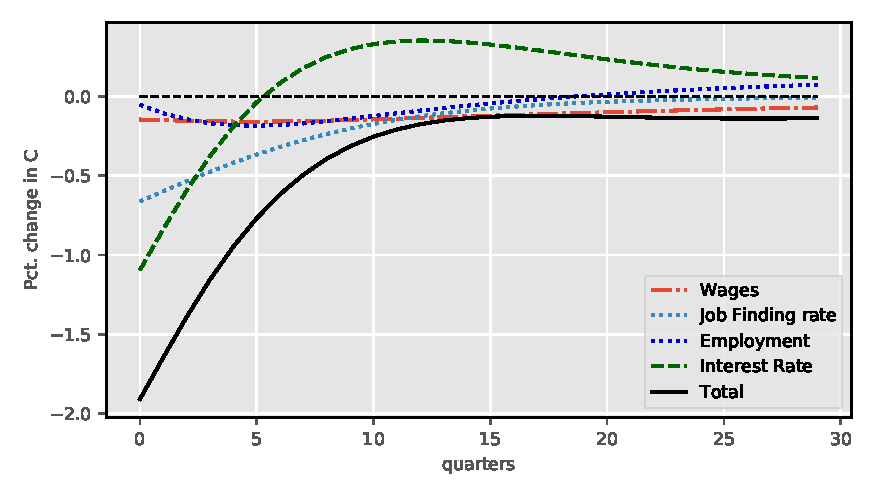
\includegraphics[width=.6\linewidth]{mainmatter/plots/SS_evaluation/C_decomp_main_G.pdf} 
}
\caption[Caption for LOF]{Decomposition of Consumption in response to a negative productivity shock. }
\label{fig:baseline_C_decomp}
\centering
\scriptsize
\centering
\emph{Note:} Decomposed responses sum to total.
\end{figure}

%Lump-sum transfers account for the majority of consumption response. This observations is common to HANK models. In \citet{kaplan2018monetary} public transfers account for roughly 1/3 of the consumption response resulting from a monetary policy shock. \\
%Half of the initial drop in consumption comes from a drop in the job finding rate through precautionary motives. The persistent drop in consumption in the following periods is driven by lower income to the household sector through different channels. 1) The government reduces transfers to satisfy debt obligations, 2) The drop in interest rates reduces financial income, and 3) A persistent drop in employment implies that more households must make due with public benefits which are roughly half of the wage rate. 


\subsection{Heterogeneity In Consumption Responses } % - Welfare Implications.
Before evaluating the welfare implications of the shock I consider the disaggregated consumption response. The left panel of Figure \ref{fig:baseline_C_decomp_disagg} displays the on-impact drop in consumption following the TFP shock by wealth deciles, along with a decomposition which serves to identify the drivers of consumption across the wealth distribution. The relative drops in consumption are monotone across wealth deciles, with the poorest households exhibiting the largest consumption drops. 
The decomposition reveals that the mechanisms behind are not entirely homogeneous. For the poorest wealth decile the largest contributing factor is higher unemployment risk, which induces precautionary savings. This channel is particularly strong for the poorest households since these are weakly insured against adverse shocks. Higher interest rates also accounts for a significant part of the decline, partly due to intertemporal substitution but also due to an increase in interest payments on debt.\footnote{Recall from the calibration that the entire 1st wealth decile are in debt.} 
As one moves up the wealth deciles the effect of increasing unemployment risk affects consumption less because households are better insured, and the defining factor becomes movements in the interest rates. 
For the wealthiest households changes in unemployment risk and wages matters very little because their asset holdings are so large that marginal utilities across employment states are always equalized. Accordingly, they almost only react to changes in the marginal rate of substitution between present and future consumption.  

%For the poorest wealth decile a large share is constrained from borrowing, and the effect of hike in the interest rate is hence lessened. Instead, the drop in the finding rate accounts for a large share of the drop in consumption for this class of workers. Since these households are poorly insured due to low savings they fear going into unemployment/staying unemployed for a longer duration more than wealthier households and the precautionary savings effect from higher labor market risk is significant. For wealthier households the higher interest rate imply that they postpone consumption, and this accounts for between 1/2-2/3 of consumption declines, with the finding rate being the second most important determinant. As shown in the consumption decomposition in figure \ref{fig:baseline_C_decomp} these considerations primarily apply to the first-period consumption response, since the drop in employment becomes more important w.r.t persistence than the finding rate. 

While the left panel of Figure \ref{fig:baseline_C_decomp_disagg} might lead one to think that stabilizing consumption is roughly equivalent with stabilizing consumption of households in bottom tail of the wealth distribution, the right panel shows that this is not necessarily the case.\footnote{When discussion stabilization in terms of stimulus to groups with high MPCs these consideration of course do not apply since MPCs are an absolute quantity, not a relative.} The change in aggregate consumption $dC_t$ can be written as an additive decomposition across wealth deciles, where each decile's contribution to the aggregate is given by $\frac{C_{i,ss}}{C_{ss}}\frac{dC_{i,t}}{C_{i,ss}}$. That is, the product of a static share $\frac{C_{i,ss}}{C_{ss}}$ (share of aggregate steady-state consumption of wealth decile $i$) and the relative change in the decile's consumption $\frac{dC_{i,t}}{C_{i,ss}}$ following the shock.\footnote{$dC_{t}=\sum_{i}dC_{i,t}\Leftrightarrow\frac{dC_{t}}{C_{ss}}=\sum_{i}\frac{1}{C_{ss}}dC_{i,t}=\sum_{i}\frac{C_{i,ss}}{C_{ss}}\frac{dC_{i,t}}{C_{i,ss}}$.} The left panel show the share of the aggregate consumption response in period 0 that each decile accounts for. This is the product of the left panel and the steady-state consumption shares (see appendix Figure \ref{fig:C_dist_by_deciles} for the steady-state distribution of consumption by wealth deciles). %Despite only accounting for 4\% of consumption the poorest households account for 15\% of the drop in aggregate consumption. For the remaining deciles the they each account for roughly an equal share. 
Despite having a consumption drop of almost 5\% the poorest decile - over double the aggregate drop of 2\% - these households have a less-than proportional affect on aggregate consumption, accounting for only 9\% of the drop. Instead the households in the lower-middle of the wealth distribution account for more than their weight, while the top decile has only a small effect on aggregate consumption. 
% More here 



%The fact that a major part of the transmission mechanism acts through transfers is not uncommon in HANK models, and is further amplified when rigid wages are present. A large part of the recent literature ignores this since wages are relatively flexible and thus accounts for a large share of the consumption response. This is for instance the case in \citet{auclert2020micro} who discusses a propagation mechanism where higher investment increases wages by increases the marginal product, thus in turn increasing consumption and output due to the high MPCs present in HANK models. 

%The reason for this relatively straightforward: While a decrease in wages hurts the government budget balance through lower income taxes, the impact is even greater when households move from employment to unemployment. Hence, when wages are more flexible and employment moves less over the cycle a smaller reduction in transfers is needed to satisfy the government budget constraint and wages thus substitute for transfers in a way. 



\begin{figure}[H]
\makebox[\linewidth][c]{%
\centering
  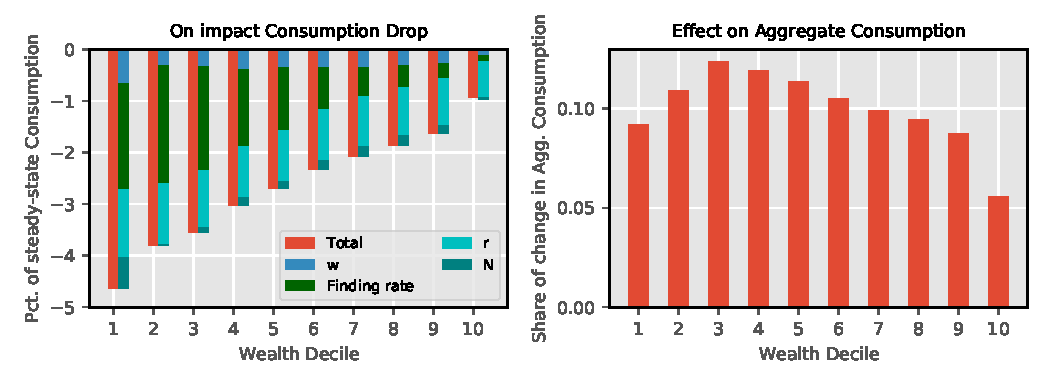
\includegraphics[width=.95\linewidth]{mainmatter/plots/SS_evaluation/peak_c_by_decile.pdf} 
}
\caption[Caption for LOF]{Decomposition of Consumption by Wealth Deciles. }
\label{fig:baseline_C_decomp_disagg}
\centering
\scriptsize 
\emph{Note:} The decomposed column might not add to the total due to first-order approximation errors.  
\end{figure}


\footnote{I first calculate the aggregate wealth deciles in the entire population. Afterwards, I divide households by employment status within each wealth decile. }


I follow \citet{gornemann2016doves} in evaluating the welfare implications of shocks. They compute lifetime consumption equivalent welfare gains/losses, defined as the amount of consumption that a given household is willing to give up to experience a certain event, here a persistent, negative TFP shock.\footnote{Let $U_{t_{0}}^{k}\left(\left\{ c_{i,t},\ell_{i,t}\right\} _{t=t_{0}}^{^{T}}\right)=\int\sum_{t=t_{0}}^{T}\beta_{i}^{t}u\left(c_{i,t},\ell_{i,t}\right)d\mathcal{D}_{t,k}$ denote discounted welfare for some group of households $k$ (percentiles, quantiles, employed, unemployed etc.) from time $t_0$ to $T$. The lifetime consumption equivalent of this group in response to the shock solves $U_{ss}^{k}\left(\left\{ \left(1+x\right)c_{i,ss},\ell_{i,ss}\right\} \right)=U_{t_{0}}^{k}\left(\left\{ c_{i,t},\ell_{i,t}\right\} _{t=t_{0}}^{^{T}}\right)$ for $x$. I use a horizon of 300 quarters, with $t_0$ being the impact period of the shock.  }
Figure \ref{fig:C_equiv_Baseline} displays the lifetime Consumption-equivalent welfare loss following the TFP shock for three different household characteristics. The left and right panel displays the losses for employed vs. unemployed households respectively. Within each panel (and employment group) I consider the welfare loss by wealth deciles, and within each wealth decile, by skill type. The skill types are the 30th, 50th, and 70th deciles in the income distribution respectively.\footnote{Note that compared to \citet{gornemann2016doves} the welfare losses do not seem to be monotone in earnings percentiles. The reason is that their figures condition on discount factors, whereas mine do not.} 

Employed households are on average willing to trade off 0.5\% of steady-state consumption to avoid the shock, while unemployed on average are willing to pay to experience the shock, though this is driven strongly by the upper wealth deciles. The main reason for this is that the shock brings about higher interest rates which households in the upper deciles benefit greatly from due to increases in financial income. For households in the bottom and lower-middle in the wealth distribution lower wages and higher unemployment risk dominates this financial income channel and they experience a welfare loss following the shock. 
There is a significant difference between the welfare implications of employed and unemployed households. For employed households only the wealthiest decile benefit from the shock, whereas for the unemployed households the 7th-9th decile also benefits from the shock. [Discuss: wages?]

% why significantly different from gorneman et al? 

%As in Gornemann et. al. I find that the welfare losses are U-shaped in wealth. That is, the largest welfare losses occur not at the bottom or top of the distribution but in the middle. The 2nd decile suffers a larger welfare drop compared to the 1st decile due to precautionary savings: Within the poorest decile a large share is constrained, and only respond to changes in income. When moving up to the second decile less households are constrained, and they respond more to drops in the job finding rate. Furthermore, they tend to be more patient (higher $\beta$)and hence "suffer" more due to the persistence of the shock, contrary to very impatient households where only drops in consumption close to $t_0$ matters.  

Recall that unemployment benefits are only proportional to idiosyncratic earnings risk, but not the aggregate wage rate $w_t$.\footnote{In practice unemployment befits are indexed to wage growth, but usually with a lag. In Denmark this occurs through the \textit{satsregulering}, where public transfers are indexed to wage growth with a two year lag.} Hence unemployed households are not subject to any income drops other than through idiosyncratic risk. 


\begin{figure}[H]
\makebox[\linewidth][c]{%
\centering
  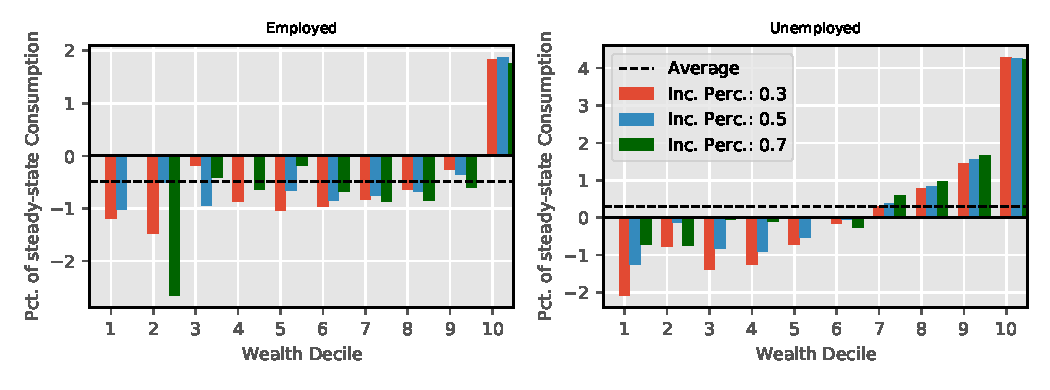
\includegraphics[width=.95\linewidth]{mainmatter/plots/SS_evaluation/C_equiv_by_e_N.pdf} 
}
\caption[Caption for LOF]{Consumption-equivalent welfare Loss by Type}
\label{fig:C_equiv_Baseline}
\centering

 % {\scriptsize  Note that the decomposed column might not add to the total due to first-order approximation errors. (Earnings percentile, employment status and wealth decile) }
\end{figure}


\subsubsection{Aggregate Inequality.} Figure \ref{fig:Inequality_response} (appendix) spells out the effects on aggregate inequality following the shock. Overall wealth and income inequality declines, but surprisingly consumption inequality increases. It is, however, notable that the share of wealth held by the top 5\% increases, and by a significant amount (0.4 percentage points at the peak). This is mainly due to the rise in interest rates since this group holds a disproportionately large share of aggregate wealth.     




%\subsubsection{Income Risk.}
%A heavily discussed feature of HANK models is income risk, and the cyclical element of it. Some papers assume acyclical risk (\citet{kaplan2018monetary}, \citet{hagedorn2019fiscal}), while others use ad-hoc, reduced form rules to model counter-cyclical risk \citet{acharya2020understanding}, \citet{auclert2018inequality}
%Pro-cyclical risk is usually not considered. My model features two separate sources of income risk: An exogenous and an endogenous channel. The exogenous channel is the earnings risk $e_i,t$ which directly affects household labor income. This gives rise to precautionary savings, but is constant over the cycle (acyclical). The endogenous channel is unemployment risk. In the presence of a search-and-matching labor market involuntary unemployment arises due to labor market frictions. In the baseline model households loose their job at an exogenous rate $\delta^L$, and re-obtain jobs at the endogenous job-finding rate $q_t$. Since the job-finding rate is counter-cyclical to the most common shocks this unemployment risk is countercyclical. The implication is that households increase savings if the job finding rate declines, and demand hence declines. This channel is extensively covered in \citet{ravn2016macroeconomic}.   



% r, Ravn and Sterk (2017), Werning (2015), Heathcote and Perri (2018), Beaudry, Galizia
%and Portier (2018), Kekre (2018), Bayer et al. (2019), Bilbiie (2019), and Acharya and Dogra (2019)   % INCLUDE Discussion


\pagebreak 
%\section{Evaluation of Automatic Stabilizers}
\section{Stabilization in the Presence of Unemployment Risk}
Incomplete markets for households along with matching frictions generates countercyclical precautionary savings as households attempts to self-insure against unemployment risk over the cycle. This section takes a closer look at how unemployment benefits - which acts as insurance against unemployment shocks - affects the economy over the business cycle. This includes both effects on aggregates in the general equilibrium and distributional and welfare effects.    

Note that unemployment risk essentially works by fluctuation households between a good state (employment) and a bad state (unemployment). When unemployment benefits are reduced the bad state becomes even worse when compared to the good state. This is comparable to the zero-income shock in \citet{carroll1997buffer}, which he argues is a significant driver of savings for precautionary  reasons. 



%I primarily focus on the stabilizing effects of unemployment benefits over the business cycle. I do this for several reasons. Unemployment benefits interact directly with the demand side through the household sector, and hence has the possibility to be a strong stabilizer since output is demand driven in the short run in NK models. Furthermore, in models with heterogeneous agents unemployment benefits affect precautionary savings motives through both income levels and labor market channels (job-finding rates). Lastly, since this particular stabilizer is associated with the redistribution of income it can be a significant source of distributional effects over the cycle.  


\subsubsection{A new Steady State}
I conduct the following experiment:
A permanent drop in the unemployment benefit rate is phased in over 100 quarters. After 300 quarters the model is assumed to have converged to a new, counterfactual steady-state which mimics the basic properties of the original steady-state, with the exception of having a lower unemployment benefit rate. To evaluate the stabilizing properties of unemployment benefits I then subject each of the steady-states to a negative TFP shock similar to the one described earlier. For unemployment benefits shock I let lump-sum transfers adjust such that the government debt-to-GDP ratio is the same as in the original steady-state (160\%).

\newcommand{\dBenefitRate}{50\%}

Figure \ref{fig:Lower_b_Transitional} in the appendix shows the responses to the permanent benefits shock. The shock lowers the benefit level by \dBenefitRate, with a phase in period corresponding to a auto-regressive parameter of 0.95.\footnote{\citet{mckay2016role} considers a  80\% reduction in  unemployment and poverty benefits.} The new steady-state is of course in itself of interest, as it touches upon the literature concerning the relation between unemployment benefits and employment, production and wages. However, in that regard the model misses the moral hazard channel of unemployment benefits affecting the extensive labor market margin, which is a major channel in this discussion. Note also that had the model included Nash-bargaining over wages, the level of unemployment benefits would have a direct effect on the bargained wage through its interpretation as the outside option. This channel is omitted in the model. \\

The drop in unemployment benefits implies a permanent drop in consumption due to lower income and precautionary savings. The drop in demand induces firm to investment less and hire less workers, so the stock of capital drops and the unemployment rate increases. This further increases the drop in consumption. The permanent increase in unemployment implies a permanently less tight labor market for firms, and hence lower wages. Since wages adjust endogenous to the drop in unemployment benefits the replacement ratio $b/w$ is in itself endogenous, and hence can be either higher or lower than the 25\% implied by the calibration and the drop in benefits of \dBenefitRate. However, according to Figure \ref{fig:Lower_b_Transitional} wages drop only marginally by 0.03\%, so the replacement rate drop by roughly \dBenefitRate - a sizeable amount.   
Relative to the old steady-state the aggregate stock of assets increase by 2.5\% for precautionary reasons. Figure \ref{fig:lower_b_dA} shows that this increase is driven entirely by employed households. The income of these households are affected only marginally in the new steady-state, but and they can thus afford to increase their insurance against unemployment through assets. This channel is strongest for households in the bottom of the wealth distribution since these are particularly poor insured to begin with. Unemployed households respond to the drop in benefits by drawing on their buffer of assets to increase consumption such that assets drop. Unemployed households at the bottom of the wealth distribution has a smaller decrease in assets due to borrowing constraints. The fact that constrained households cannot insure to the extent of their wish potentially imply large welfare losses. 

\begin{figure}[H]
\makebox[\linewidth][c]{%
\centering
  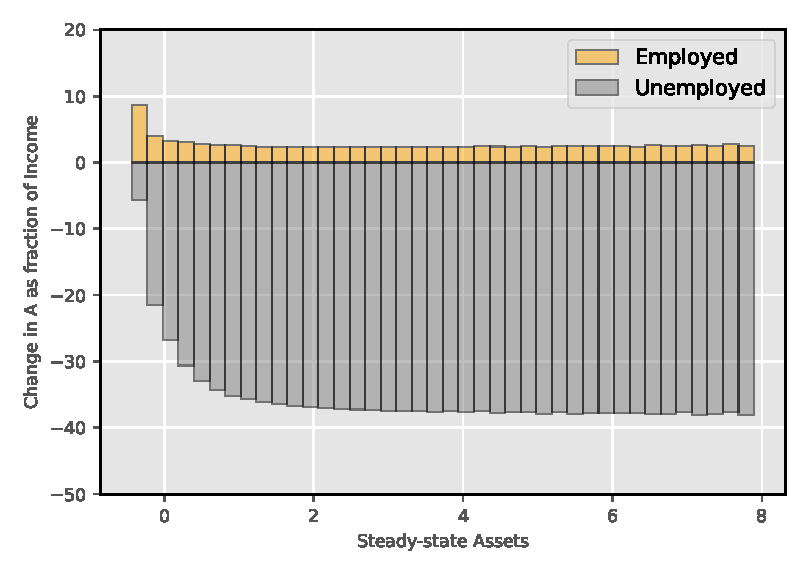
\includegraphics[width=.6\linewidth]{mainmatter/plots/Lower_b_main/dA.pdf} 
}
\caption[Caption for LOF]{Change in Assets by initial steady-state assets.}
\label{fig:lower_b_dA}
 % {\scriptsize  Impulse responses to a negative productivity shock of 1\% with persistence 0.94 (half-life: 5 quarters). }
\end{figure}

Figure \ref{fig:Lower_b_Transitional} shows the estimated transitional dynamics using both linear and non-linear methods. Due to the size of the shock non-linearities matter, and I hence use the non-linear method to iterate to the new steady state. 


\subsubsection{Unemployment Benefits as a Stabilizer}
Having numerically obtained the new steady state with a lower level of unemployment benefits, I now investigate the stabilizing properties of these benefits. Figure \ref{fig:lower_b_main} compares negativity productivity shock (1\% with persistence 0.8) in the baseline model and the model with lower unemployment benefits.
The on-impact drop in consumption is greatly affected by the amount if unemployment insurance (-2\% vs -2.5\%), though the afterwards persistence is roughly the same. This drop in demand leads to larger drops in employment and output, though investment seems to be unaffected. The reduction of labor demand diminishes job-finding opportunities, and the labor market becomes less tight from the point of view of firms. This leads to a further drop in wages and hours worked. The drop in employment and output implies a slight drop in marginal costs and hence inflation. In turn, the central bank raises the interest rate less. 

%Somewhat surprisingly given the size of the shock to benefits, the remaining business cycle variables are relatively unaffected, and the majority are actually stabilized by the lower level of benefits. This derives primarily from a general equilibrium effect working through the governments budget. As the economy deteriorates following the shock, unemployment rises and hence public expenses associated with unemployment benefits increases. This is primarily financed by issuing debt, but also by cutting government spending. In the model with lower benefits the expenditure side of the government budget suffers less and public consumption is cut by less. Since this is in itself a component of aggregate demand, there is a slight drop in volatility. The reduced volatility in employment, job finding rates etc. is, however not sufficient to counter the drop in consumption occurring through the lower value of unemployment. 



%The immediate conclusion is that the level of unemployment benefits and hence the replacement ratio does not affect the persistence of shocks, and does little towards the size and propagation of the negative investment shock. While the quantitative effects are small, the qualitative effects reflect that unemployment benefits does serve a purpose as a stabilizer: It lessens the drop in consumption, output and employment.  

\begin{figure}[H]
\makebox[\linewidth][c]{%
\centering
  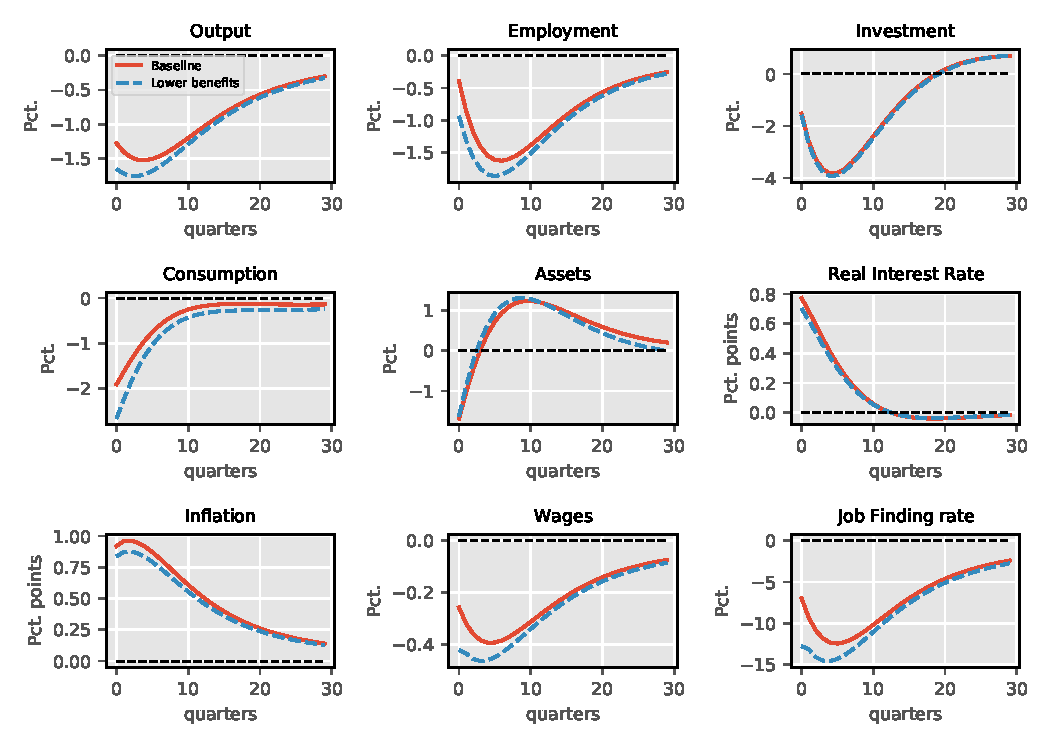
\includegraphics[width=.8\linewidth]{mainmatter/plots/Lower_b_main/main_result_comparison_G.pdf} 
}
\caption[Caption for LOF]{Impulses to a negative TFP shock with standard and low unemployment benefits.}
\label{fig:lower_b_main}
 % {\scriptsize  Impulse responses to a negative productivity shock of 1\% with persistence 0.94 (half-life: 5 quarters). }
\end{figure}

%Unemployment benefits directly affect the model into places: The income process of household and the government's budget constraint. Figure \ref{fig:lower_b_C_decomp} 


Figure \ref{fig:lower_b_C_decomp_G} decomposes the aggregate response of consumption. The figure reveals that the level of unemployment benefits is important for the response of consumption to changes in employment and job-finding opportunities. The drop in job-finding rates has a strong, immediate negative effect on consumption (roughly double the effect on impact) under lower benefits due to a stronger precautionary motive: For employed households lower job-finding rates imply that if they drop into unemployment exogenously their odds of bouncing back into employment diminishes. Hence they buffer up on assets by cutting consumption to ensure against this increased risk. For unemployed households future employment prospects drop, and they increase savings to accommodate a longer unemployment spell. A more severe drop in employment in the general equilibrium generates a more persistent drop in consumption since unemployed households on average has lower consumption.\footnote{At a benefit rate of 51\% (the baseline model) unemployed households has on average 86\% the consumption of employed households. After the cut in benefits this figure drop to 80\%.} Wages decline more in the general equilibrium of the modified model and this leads to a larger consumption drop. The response of consumption to changes the interest is roughly the same. 

Essentially, the drop in unemployment benefits have not dramatically large effects in the general equilibrium because households manage to self-insure against unemployment risk. 

\begin{figure}[H]
\makebox[\linewidth][c]{%
\centering
  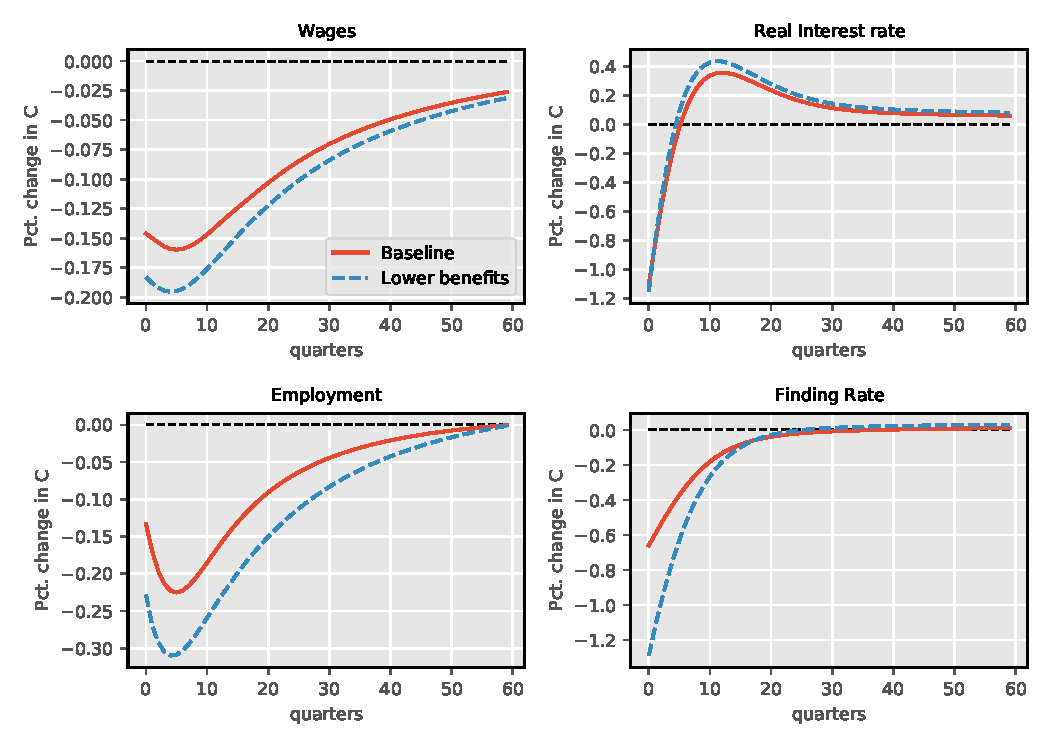
\includegraphics[width=.98\linewidth]{mainmatter/plots/Lower_b_main/main_result_C_decomp_G.pdf} 
}
\caption[Caption for LOF]{Consumption Decomposition.}
\label{fig:lower_b_C_decomp_G}
 % {\scriptsize  Impulse responses to a negative productivity shock of 1\% with persistence 0.94 (half-life: 5 quarters). }
\end{figure}




\subsubsection{Welfare Implications.}



\begin{figure}[H]
\makebox[\linewidth][c]{%
\centering
  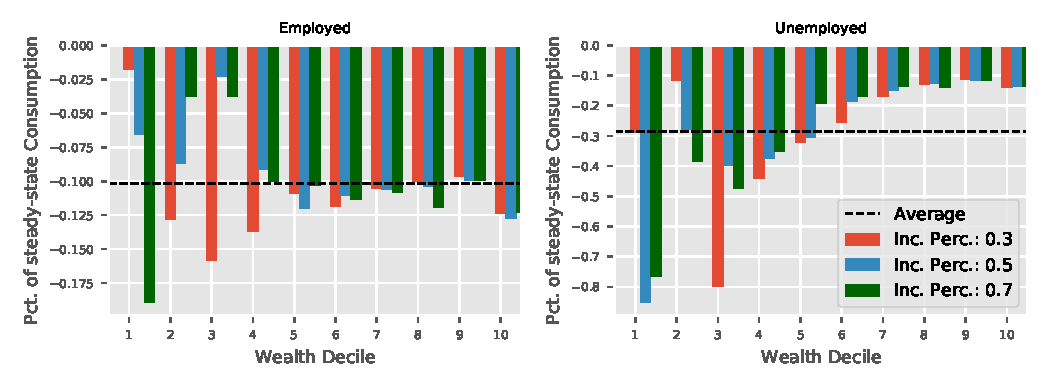
\includegraphics[width=.98\linewidth]{mainmatter/plots/Lower_b_main/equiv_welfare.pdf} 
}
\caption[Caption for LOF]{Consumption equivalent welfare losses from cutting unemployment benefits.}
\label{fig:lower_b_C_decomp_G}
 % {\scriptsize  Impulse responses to a negative productivity shock of 1\% with persistence 0.94 (half-life: 5 quarters). }
\end{figure}

\subsubsection{Aggregate Inequality.} Figure \ref{fig:Inequality_response_lower_b} in the appendix compares the changes in aggregate inequality. With lower unemployment insurance poor households save more for precautionary reasons and w
Consumption inequality increases as poor households cut consumption for precautionary reasons, but the aggregate effects are still neglectable.  





\subsection{Tax Financing}
The presence of heterogeneous households imply Ricardian equivalence does not hold in this model, and financing government activities with taxes versus bonds alter the dynamic responses of shocks. Though I consider the scenario where the government fiances its expenses by primarily issuing bonds as the baseline scenario, I here consider the alternative. At each instant in time the government adjusts lump-sum transfers, to be distributed uniformly across households, to satisfy their government constraint. This is standard in simpler NK models. 
Figure \ref{fig:lower_b_shocks_T} presents the general equilibrium outcomes. There is slight propagation in the first period for output, consumption, employment and job-finding rates, though the overall impulses are roughly unchanged under a lower benefit level. 
The decomposition in Figure \ref{fig:lower_b_C_decomp_T} shows that compared to the bonds-financing scenario, wages and transfers now determine the majority of the consumption response, with the effect of interest rate on consumption being roughly halved. Regarding the effects of unemployment benefits the conclusions are almost unchanged: A more volatile job-finding rate propagates the initial consumption decline, while a slightly more persistent employment slump generates a more persistent drop in consumption. The effects of wages, transfers and interest rates on consumption are the same.  


\begin{figure}[H]
\makebox[\linewidth][c]{%
\centering
  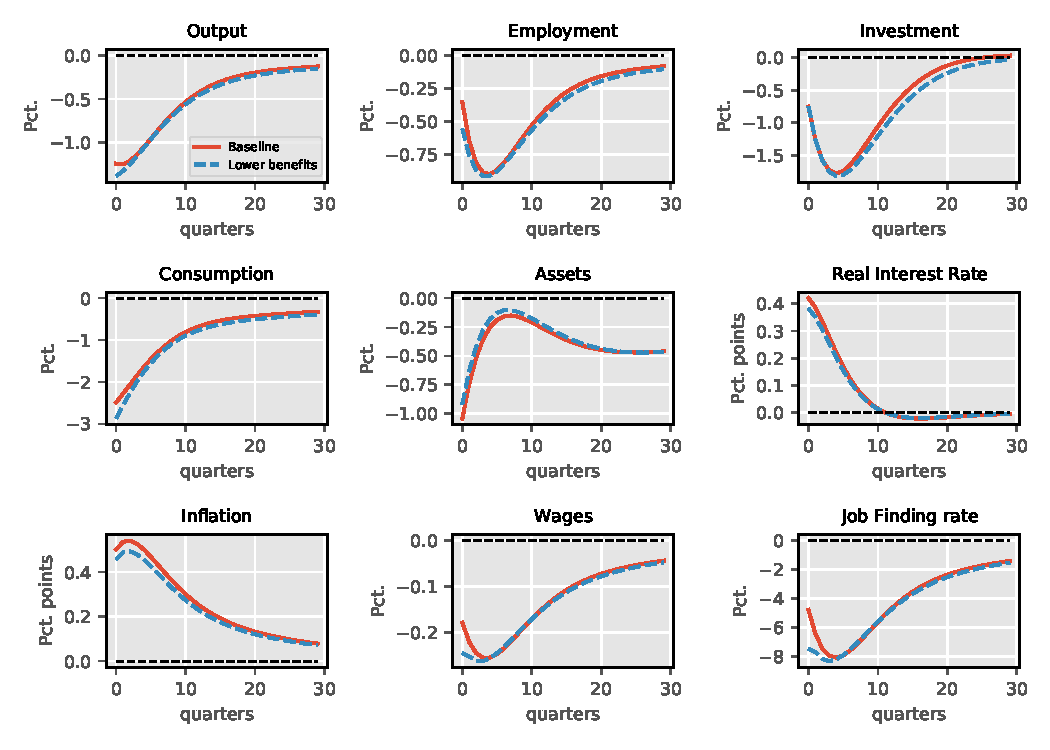
\includegraphics[width=.8\linewidth]{mainmatter/plots/Lower_b_main/main_result_comparison_T.pdf} 
}
\caption[Caption for LOF]{Consumption Decomposition.}
\label{fig:lower_b_shocks_T}
 % {\scriptsize  Impulse responses to a negative productivity shock of 1\% with persistence 0.94 (half-life: 5 quarters). }
\end{figure}


\begin{figure}[H]
\makebox[\linewidth][c]{%
\centering
  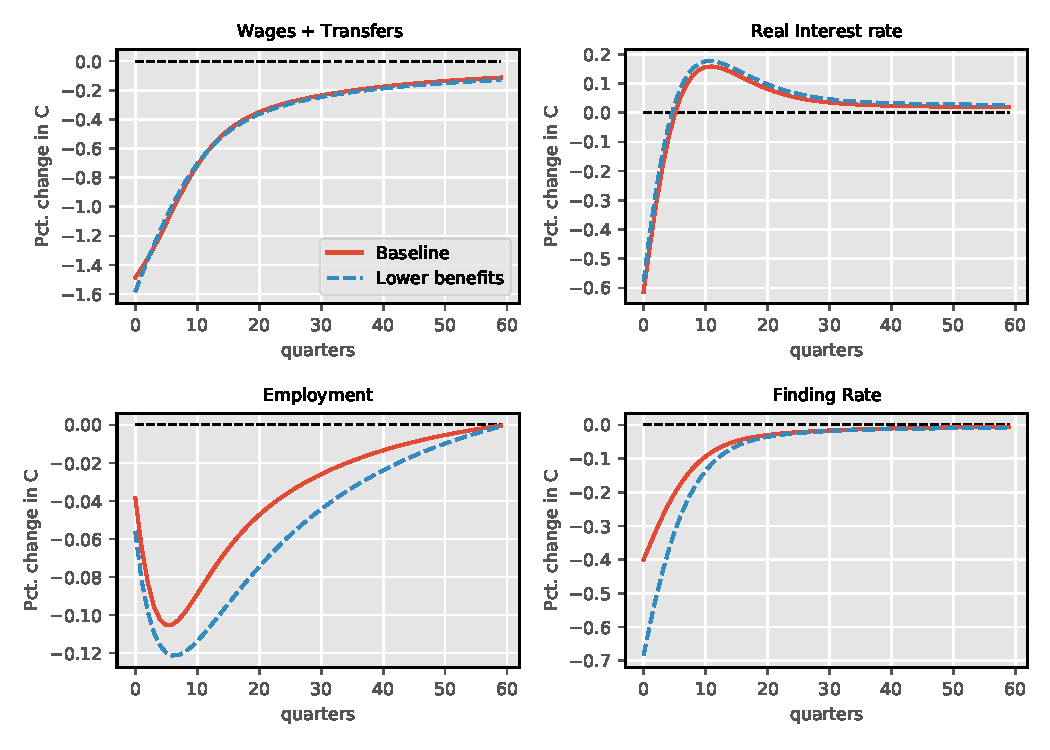
\includegraphics[width=.8\linewidth]{mainmatter/plots/Lower_b_main/main_result_C_decomp_T.pdf} 
}
\caption[Caption for LOF]{Consumption Decomposition.}
\label{fig:lower_b_C_decomp_T}
 % {\scriptsize  Impulse responses to a negative productivity shock of 1\% with persistence 0.94 (half-life: 5 quarters). }
\end{figure}


   % INCLUDE Discussion


\pagebreak 
\section{Matching Dynamics}
The baseline model of the search-and-matching labor market implicitly assumes free-entry for labor market firms, such that value of posting a vacancy is zero in equilibrium. This, in conjunction with linear vacancy posting costs, imply that the dynamic response of vacancies tend to be highly volatile and short lived. This is generally considered to be incompatible empirical responses of vacancies and unemployment rates, see for instance the general discussion in \citet{elsby2015beveridge}.


\subsection{Beveridge Curve}

Figure \ref{fig:Beveridge_cruve_data} shows the empirical Beveridge curve for the US 1951-2003. Conditioning on historical time periods the figure displays a clear negative correlation between the vacancy rate and the unemployment rate. In the context of search-and-matching models this is interpreted as the presence of pro-cyclical market tightness. That is, during an economic boom firms demand more labor through an increase in vacancy postings, but given decreasing returns to vacancies alone in the matching function firms must post an increasingly higher number of vacancies to increase their labor stock.\footnote{There is constant returns to the overall matching function so market tightness is not pro-cyclical if the numbers of searchers is sufficiently elastic. However, } This general a negative relationship between vacancy posting and the unemployment rate.




\begin{figure}[H]
\makebox[\linewidth][c]{%
\centering
  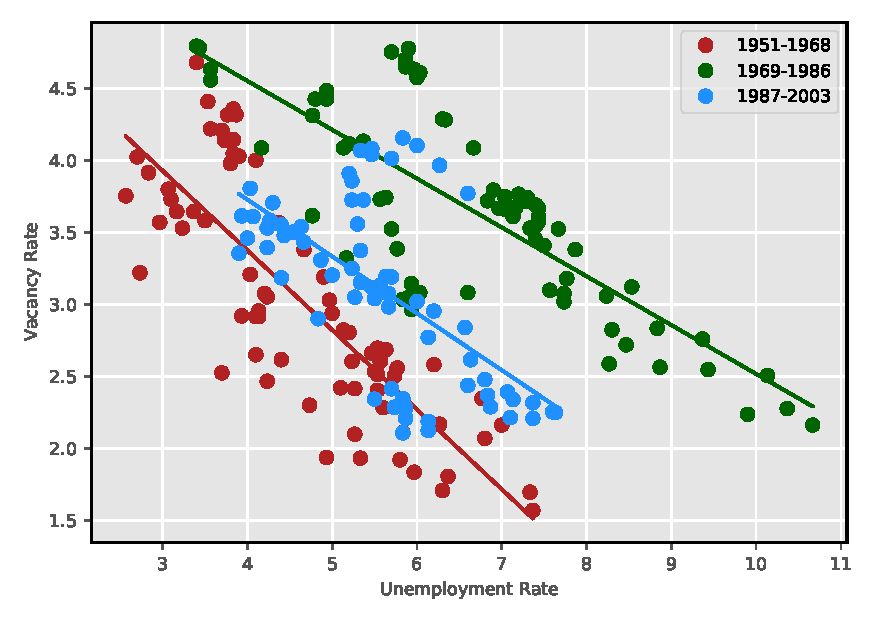
\includegraphics[width=.8\linewidth]{mainmatter/plots/Labor_market/Beveridge.pdf} 
}
\caption[Caption for LOF]{US Beveridge Curves 1951-2003}
\label{fig:Beveridge_cruve_data}
\centering
  {\scriptsize US Beveridge curve 1951-2003. The vacancy rate is proxied by the \textit{Composite Help-Wanted Index} from \citet{barnichon2010building}. The unemployment rate is obtained from FRED.  }
\end{figure}

\footnote{Since the model contains no aggregate shocks the Beveridge curve cannot be obtained through stochastic simulations. }

The empirical Beveridge curve is generated by a wide array of different shocks. In the theoretical framework presented earlier, I have primarily focused on a neutral technology shock.  


One way to generate non-jump dynamics of vacancies is to assume costly entry as in \citet{coles2018job}. A simpler way to generate more persistent dynamics in vacancy posting is to add quadratic costs to vacancy posting, contrary to the usual linear specification. Conjecturing that all firms choose the same amount of vacancies in equilibrium, the cost of posting vacancies is given by $\frac{\kappa_{V}}{2}V_{t}^{2}$. Labor demand obeys the same optimality condition as before:
\begin{gather*}
\mathcal{J}_{t}^{m}=\left(MPL_{t}-w_{t}h_{t}\right)+\frac{\left(1-\delta^{\text{L}}\right)}{1+r_{t+1}}\mathcal{J}_{t+1}^{m},,
\end{gather*}
where $\mathcal{J}_{t}^{m}$ measures the value of a match. Adding quadratic costs of vacancy posting affects only the optimal value of match, which is now given by $\mathcal{J}_{t}^{m}=\frac{\kappa_{V}V_{t}}{m_{t}}$, compared to $\mathcal{J}_{t}^{m}=\frac{\kappa_{V}}{m_{t}}$ from before.





To closer match the persistence observed in the data I follow \citet{fujita2007job} in modifying the vacancy creation process. 

Firms that want to enter the labor service sector must pay an additional cost $\kappa^{x}x_{t}$ where $x_t$ is the number of open positions in the economy at time $t$. The purpose of vacancies are to fill open positions. These can be open either because they have been created recently or because an existent match has been terminated through exogenous job destruction. Positions exist until they are terminated through obsolescence. 
Let $\delta^{O}$ denote the rate of job obsolescence. Let $\delta^{NO}$ denote the probability that a match is destroyed but the position not terminated. The job destruction rate that prevails at the aggregate level is given by $\delta^{N}=\delta^{O}+\left(1-\delta^{O}\right)\delta^{NO}$. That is, the sum of the probability that a job is destroyed by obsolesce $\delta^{O}$ and the probability that a match is destroyed given that the position is not made obsolete $\left(1-\delta^{O}\right)\delta^{NO}$. 

For households that are unemployed at time $t$ the probability of obsolescence imply that the Euler equation now reads:
\begin{gather*}
\left(c_{i,t}^{k=U}\right)^{-\frac{1}{\sigma}}=\beta\mathbb{E}_{i,t}R_{t+1}\left[\left(1-\delta^{O}\right)q_{t+1}\left(c_{i,t+1}^{k=N}\right)^{-\frac{1}{\sigma}}+\left(1-\left(1-\delta^{O}\right)q_{t+1}\right)\left(c_{i,t+1}^{k=U}\right)^{-\frac{1}{\sigma}}\right]
\end{gather*}
which reads that the households obtains employment with probability $q_t+1$ times the probability that the position is not made obsolete. The probability of remaining in unemployment is the complementary probability. Hence the new addition is that an unlucky share $\delta^{O}q_{t+1}$ of time $t$ searchers will find a job in the subsequent period, but this job will be made obsolete immediately. 
For employed households the Euler reads the same:
\begin{gather*}
\left(c_{i,t}^{k=N}\right)^{-\frac{1}{\sigma}}=\beta\mathbb{E}_{i,t}R_{t+1}\left[\left(1-\delta^{N}\left(1-q_{t+1}\right)\right)\left(c_{i,t+1}^{k=N}\right)^{-\frac{1}{\sigma}}+\delta^{N}\left(1-q_{t+1}\right)\left(c_{i,t+1}^{k=U}\right)^{-\frac{1}{\sigma}}\right]
\end{gather*}
though the job destruction rate $\delta^{N}$ has been redefined to include both destruction from obsolescence and from the termination of matches.  
The law of motion for employment reads:
\begin{gather*}
N_{t}=\left(1-\delta^{N}\right)N_{t-1}+S_{t}q_{t}\left(1-\delta^{O}\right),
\end{gather*}
which is only modified by the term $\left(1-\delta^{O}\right)$. 
Compared to the canonical search-and-matching model, where vacancies are a flow/jump variable, the above assumptions introduce a few additional dynamics for vacancies. Period $t$ vaccines $V_t$ is the sum of several flows: 
\begin{gather*}
V_{t}=\left(1-\delta^{O}\right)V_{t-1}+\left(1-\delta^{O}\right)\delta^{NO}N_{t-1}-\left(1-\delta^{O}\right)m_{t-1}V_{t-1}+x_{t}
\end{gather*}
taking them from left to right, the terms are: previous vacancies that have not been made obsolete $\left(1-\delta^{O}\right)V_{t-1}$, 
new vacancies that must be posted for positions that still exist but where the match has been terminated $\left(1-\delta^{O}\right)\delta^{NO}N_{t-1}$, vacant positions that were not made obsolete but were matched $\left(1-\delta^{O}\right)m_{t-1}V_{t-1}$ need not be filled again, the creation of $x_t$ new positions imply $x_t$ new vacancies must be posted. 

Given the redefinition of the job destruction rate the firms value of a match is unchanged:
\begin{gather*}
\mathcal{J}_{t}^{m}=\left(MPL_{t}-w_{t}\right)+\frac{\left(1-\delta^{N}\right)}{1+r_{t+1}}\mathcal{J}_{t+1}^{m},
\end{gather*}
Free entry imply that the value of a match must equal the cost $\mathcal{J}_{t}^{m}=\frac{\kappa_{V}V_{t}+\kappa_{x}x_{t}}{m_{t}}$. Since the cost posting vacancies and job openings affect the value of a match similarly they cannot both be identified from the steady-state. I hence set $\kappa_{V}=0$. 


\subsubsection{Calibration.} \citet{fujita2007job} finds that normal job destruction and obsoleting account for roughly and equal half of aggregate job destruction. I use this relation ship and set $\delta^{O}=\delta^{N}\frac{1}{2}$, where $\delta^{N}=0.06$ is the empirical estimate of the aggregate job destruction rate from XXX. The "normal" job destruction rate is then found residually as $\delta^{NO}=\frac{\delta^{N}-\delta^{O}}{1-\delta^{O}}$. The remaining calibration of the labor market is the same as earlier, though the calibrated job-finding rate changes slightly since the flow out of unemployment is affected by the job obsolesce rate.    % INCLUDE Discussion

%


\pagebreak 
\section{Cyclical Wage Inequality}
\label{chap:Autostab_base}




\subsection{Cyclical Wage Dispersion} % widening earnings distribution cycle
In the baseline model all households are affected equally by changes in the aggregate wage rate. Additionally, the model assumes that a law of large numbers apply at the aggregate level such that firms hire the average worker. Households make no search decision and I rule out on the job search, so all households are subjected equally to job destruction and hiring. Resultingly, employment dynamics have no distributional effects either and business cycles are "neutral" per se. There exists a multitude of reasons why this is not necessarily the case. Agents in different parts of the earnings distribution might differ structurally in terms of age, education, geographical placement, gender and this might effect wages and employment status over the business cycle. The most obvious case occurs when agents have heterogeneous wages due to being employed in different sectors. \\

There are different ways to micro-found such mechanisms. One is on-the-job search as in \citet{moscarini2017job}. \citet{hubmer2018job} shows that a partial equilibrium model with on-the-job search generates a job-ladder type model. This type of model generates significantly more earnings risk in an endogenous way and fits the data better as opposed to the usual exogenous AR(1) processes for earnings risk with log-normal innovations. The addition of a search and matching labor market also aids in this regard, but only marginally through the job-finding rate. 



% Guvernen
\citet{guvenen2014nature} finds that income risk (as measured by the variance of household earnings) is acyclical. However, they document cyclical responses in the tails of the distribution. They find that the distribution of shocks become more left-skewed in recessions, implying that large positive shocks becomes less likely and adverse, negative shocks become more likely. This primarily related to within-group (earnings percentile) dispersion. For between-group dynamics, they find that earnings are most cyclical at the bottom and the absolute top of the earnings distribution. To this end, figure \ref{fig:Song_et_al} displays estimated elasticities of earnings to GDP from \citet{guvenen2017worker} as a measure of cyclicality by earnings percentiles. 

%31 Our model would feature an additional source of amplification if we introduced unequal income incidence, making
%income inequality countercyclical (see Bilbiie, Känzig and Surico 2019) - from micro jumps macro humps 

%It is worth noting that while Guvenen et al. (2014) find that the variance of household income is
%acyclical, they find that the left-skewness is countercyclical. Given our assumption of normally distributed
%income, skewness is constant in our model


%That is, during recessions, the
%upper end of the shock distribution collapses—large upward income movements become less likely—
%whereas the bottom end expands—large drops in income become more likely. Thus, while the dispersion
%of shocks does not increase, shocks become more left skewed and, hence, risky during recessions


\begin{figure}[H]
\makebox[\linewidth][c]{%
\centering
  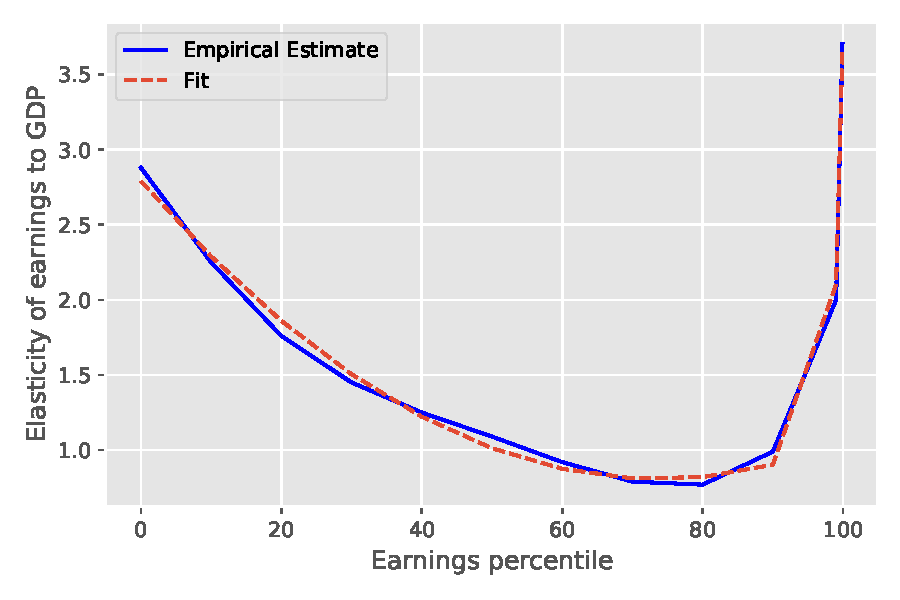
\includegraphics[width=.5\linewidth]{mainmatter/plots/cyclical_earnings/Song_earnings_cyclical.pdf} 
}
\caption{Estimated elasticity of earnings to GDP by percentile from \citet{guvenen2017worker}.}
\label{fig:Song_et_al}
 % {\scriptsize  Impulse responses to a negative productivity shock of 1\% with persistence 0.94 (half-life: 5 quarters). }
\end{figure}


Recent HANK models introduce endogenous, cyclical movements in the earnings distribution in ad-hoc manners. Analytical papers such as \citet{acharya2020understanding} assumes that the variance of labor supply depends on aggregate output. \citet{auclert2018inequality} does so by assuming that labor income contains a term $\gamma\left(e_{i,t},Y_{t}\right)$ that redistributes across the earnings distribution in response to cyclical changes as measured by $Y_t$.
Labor income in the two employment states are then given by $w_{t}\ell_{i,t}e_{i,t} \gamma\left(e_{i,t},Y_{t}\right)$ and $be_{i,t}\gamma\left(e_{i,t},Y_{t}\right)$. The function satisfies $\gamma\left(e_{i,t},Y^{ss}\right)=1$ such that there is no redistribution in steady-state. Furthermore $\gamma\left(e_{i,t},Y_{t}\right)=1$ for all $e_{i,t}$ such that the incidence function only redistributes across the earnings distribution but do not affect or alter aggregate income flows. 


Whether the incidence function introduces additional propagation or reduces volatility over the cycle is ambiguous. Households at the bottom of the earnings distribution tend to have higher MPCs whereas households at the top have low MPCs, and the effect on aggregate consumption hence depends on whether which of these effects dominate.  



%We introduce on-the-job search frictions in an otherwise standard monetary DSGE
%New-Keynesian model. Heterogeneity in productivity across jobs generates a job ladder. Firms Bertrand-compete for employed workers using the Sequential %Auctions protocol of Postel-Vinay and Robin (2002). Outside job offers to employed workers, when
%accepted, reallocate employment up the productivity ladder; when declined, because
%matched by the current employer, they raise production costs and, due to nominal
%price rigidities, compress mark-ups, building inflationary pressure. When employment
%is concentrated at the bottom of the job ladder, typically after recessions, the reallocation effect prevails, aggregate supply expands, moderating %arginal costs and inflation.
%As workers climb the job ladder, reducing slack in the employment pool, the inflation
%effect takes over. The model generates endogenous cyclical movements in the Neo
%Classical labor wedge and in the New Keynesian wage mark-up. The economy takes
%time to absorb cyclical misallocation and features propagation in the response of job
%creation, unemployment and wage inflation to aggregate shocks.   % INCLUDE Discussion

%


\pagebreak 
\section{Additional Labor Market Frictions}

\citet{Jeppe2020}



\subsection{Model}
\subsubsection{Matching Process}
In the expanded model vacancies are modelled as a stock, and thus obeys the law of motion:
\begin{gather*}
V_{t}=\underline{V}_{t}+\iota_{t}, 
\end{gather*}
where $\underline{V}_{t}$ is the start-of-period stock of vacancies and $\iota_{t}$ is the number of new vacancies posted. $V_t$ is the relevant vacancy measure for matching, which still occurs through the Cobb-Douglas function $M_{t} = \mathcal{M} S_{t}^{\xi}V_{t}^{1-\xi}$. As before, let $m_t$ denote the matching probability and $q_t$ the job finding rate. The post-matching levels of unemployment and vacancies are:
\begin{gather*}
U_{t}=\left(1-q_{t}\right)S_{t}, \\
\tilde{V}_{t}=\left(1-m_{t}\right)V_{t}
\end{gather*}
Finally, an endogenous share of jobs $\delta^L_t$ are lost at the end of the period, and similarly vacancies are destroyed at an exogenous rate $\delta^V$. The number of searchers and vacancies at the start of the next period is then given by:
\begin{gather*}
S_{t+1}=U_{t}+\delta_{t}^{L}N_{t}, \\
\underline{V}_{t+1}=\left(1-\delta^{V}\right)\tilde{V}_{t}
\end{gather*}
 

\subsubsection{Matching Value}
Let $\mathcal{V}_{t}^{M}$ denote the time $t$ value of a match. At the end of the period each firm must pay a continuation cost $\chi_{t}$ to keep its match, or else it is destroyed. The continuation cost is stochastic and has cumulative distribution function $G$. Firms pay the contiuation cost if the expected value of keeping the match out weights the cost, $\frac{1}{1+r_{t+1}}\mathbb{E}_{t}\mathcal{V}_{t+1}^{M}>\chi_{t}$. Optimally entails that the value of a match is given by the bellman equation:
\begin{align*}
\mathcal{V}_{t}^{M}&=\frac{\partial div_{t}}{\partial N_{t}}+\int^{\chi_{c,t}}\left[\frac{1}{1+r_{t+1}}\mathbb{E}_{t}\mathcal{V}_{t+1}^{M}-\chi_{t}\right]dG\left(\chi_{t}\right) \\
&=mc_{t}\frac{\partial Y_{t}}{\partial N_{t}}-w_{t}+\int^{\chi_{c,t}}\left[\frac{1}{1+r_{t+1}}\mathbb{E}_{t}\mathcal{V}_{t+1}^{M}-\chi_{t}\right]dG\left(\chi_{t}\right),
\end{align*}
where $\chi_{c,t}=\frac{1}{1+r_{t+1}}\mathbb{E}_{t}\mathcal{V}_{t+1}^{M}$ is the cutoff above which firms do not pay the cost, and matches are destroyed. Accordingly, $G\left(\chi_{c,t}\right)$ is the number of matches kept for next period, such that $1-G\left(\chi_{c,t}\right)$ equals the endogenous job destruction rate, $\delta_{t}^{L}=1-G\left(\chi_{c,t}\right)$. Letting $\mu_{t}=\int^{\chi_{c,t}}\chi_{t}dG\left(\chi_{t}\right)$ denote the average continuation cost the Bellman equation can be restated as: 
\begin{gather*}
\mathcal{V}_{t}^{M}=mc_{t}\frac{\partial Y_{t}}{\partial N_{t}}-w_{t}+\frac{1-\delta_{t}^{L}}{1+r_{t+1}}\mathbb{E}_{t}\mathcal{V}_{t+1}^{M}-\mu_{t}
\end{gather*}


\subsubsection{Vacancy Creation}
The following Bellman equation describes the firm value of a vacancy post:
\begin{gather*}
\mathcal{V}_{t}^{V}=\mathcal{V}_{t}^{M}m_{t}-\kappa^{V}+\frac{\left(1-m_{t}\right)\left(1-\delta^{V}\right)}{1+r_{t+1}}\mathbb{E}_{t}\mathcal{V}_{t+1}^{V}
\end{gather*}
The model also contains entry costs for labor market firms. Each period a constant number of candidate firms $F$ draw a stochastic entry cost $c$ distributed in according to $H$. Firms pay the entry cost and pay vacancies if and only if $\mathcal{V}_{t}^{V}\geq c$, such that the number of new vacancies posted is:
\begin{gather*}
\iota_{t}=H\left(\mathcal{V}_{t}^{V}\right).
\end{gather*}   % INCLUDE Discussion

% References 
\pagebreak 
%\addcontentsline{toc}{chapter}{Bibliography}
\section{Bibliography}
%\vspace{1cm}
%\printbibliography[heading=none]

\bibliography{refs}

 

% Appendix 
\pagebreak 
\renewcommand{\appendixname}{\centering Appendix}
\renewcommand{\appendixpagename}{\centering Appendix}
\renewcommand{\appendixtocname}{Appendix}


\begin{appendices}
\counterwithin{figure}{section}
%\addtocontents{toc}{\protect\setcounter{tocdepth}{0}}
\addtocontents{toc}{\def\protect\cftchappresnum{\appendixname{} }}




\section{Model Derivations}


\subsection{Firm First-order Conditions}
\subsubsection{Pricing}
Let $\eta$ be the Lagrange multiplier associated with the constraint $y_{j,t}=\left(\frac{p_{j,t}}{P_{t}}\right)^{-\frac{\mu_{p}}{\mu_{p}-1}}Y_{t}$. The first-order condition for prices $p_{j,t}$ is:
\begin{align*} 
\frac{\partial\mathcal{L}_{t}}{\partial p_{j,t}}=&\left(1-\tau^{c}\right)\left\{ \frac{y_{j,t}}{P_{t}}-\frac{\mu_{p}}{\mu_{p}-1}\frac{1}{\epsilon_{p}}\left[\ln\left(1+\pi_{j,t}\right)\right]Y_{t}\frac{1}{1+\pi_{j,t}}\frac{1}{p_{j,t-1}}\right. \\
&+\left.\frac{1}{1+r_{t+1}}\left[-\frac{\mu_{p}}{\mu_{p}-1}\frac{1}{\epsilon_{p}}\left[\ln\left(1+\pi_{j,t+1}\right)\right]Y_{t+1}\frac{1}{1+\pi_{j,t+1}}\left(-\frac{p_{j,t+1}}{p_{j,t}^{2}}\right)\right]\right\} \\
&-\eta_{t}\left[-\left(-\frac{\mu_{p}}{\mu_{p}-1}\right)\left(\frac{p_{j,t}}{P_{t}}\right)^{-\frac{\mu_{p}}{\mu_{p}-1}-1}\frac{Y_{t}}{P_{t}}\right]=0
\end{align*}
Define $mc_{t}\equiv 1-\frac{\eta_{t}}{1-\tau^{c}}$ and simplify, to get the forward looking, New Keynesian Philips curve:
\begin{align*} 
\ln\left(1+\pi_{j,t}\right)=\epsilon_{p}\left(mc_{t}-\frac{1}{\mu_{p}}\right)+\frac{1}{1+r_{t+1}}\left[\ln\left(1+\pi_{j,t+1}\right)\right]\frac{Y_{t+1}}{Y_{t}}
\end{align*}


\subsubsection{Capital Demand}
The first-order condition for capital is:
\begin{gather*}
\frac{\partial\mathcal{L}_{t}}{\partial k_{j,t}}=\left(1-\tau^{c}\right)\left\{ \frac{p_{j,t}}{P_{t}}\frac{\partial y_{j,t}}{\partial k_{j,t}}-r_{t}^{k}\right\} -\eta_{t}\left[\frac{\partial y_{j,t}}{\partial k_{j,t}}\right]=0 \\
\alpha\frac{Y_{t}}{K_{t}}mc_{t}=r_{t}^{k}
\end{gather*}


\subsubsection{Vacancy posting and labor demand}
The vacancy posting FOC is: 
\begin{align*}
\frac{\partial\mathcal{L}_{t}}{\partial v_{j,t}}=-\left(1-\tau^{c}\right)\epsilon_{L}+\Xi_{t}m_{t}=0 \\
\Leftrightarrow\left(1-\tau^{c}\right)\epsilon_{L}=\Xi_{t}m_{t}  
\end{align*}
The FOC for labor demand is:
\begin{gather*}
\frac{\partial\mathcal{L}_{t}}{\partial n_{j,t}}=\left(1-\tau^{c}\right)\left\{ \frac{p_{j,t}}{P_{t}}\frac{\partial y_{j,t}}{\partial l_{j,t}}-w_{t}\right\} -\eta_{t}\left[\frac{\partial y_{j,t}}{\partial l_{j,t}}\right]-\Xi_{t}+\frac{1}{1+r_{t+1}}\Xi_{t+1}\left(1-\delta^{\text{L}}\right)=0
\end{gather*}
Combining this, and the vacancy posting FOC gives:
\begin{gather*}
\left(1-\alpha\right)\frac{Y_{t}}{N_{t}}mc_{t}=w_{t}+\frac{\epsilon_{L}}{m_{t}}-\frac{\left(1-\delta^{\text{L}}\right)}{1+r_{t+1}}\frac{\epsilon_{L}}{m_{t+1}}    
\end{gather*}


\subsubsection{Capital firms - Capital supply}
Capital firms max the objective function:
\begin{align*}
V_{t}^{K}\left(K_{t-1},K_{t},I_{t-1},I_{t},I_{t+1}\right)=&\max_{K_{t},I_{t}}D_{t}^{K}\left(K_{t-1},I_{t-1},I_{t}\right)+p_{t}^{K}\left(K_{t},I_{t},I_{t+1}\right) \\
&+\frac{1}{1+r_{t+1}}V_{t+1}^{K}\left(K_{t},K_{t+1},I_{t},I_{t+1},I_{t+2}\right)
\end{align*}
subject to capital accumulation $K_{t}=\left(1-\delta\right)K_{t-1}+Z_{t}^{I}I_{t}$, and where dividends are given by:
\begin{gather*}
D_{t}^{K}\left(K_{t-1},I_{t-1},I_{t}\right)=r_{t}^{k}K_{t-1}-I_{t}\left(1+\phi_{I}\left(\frac{I_{t}}{I_{t-1}}\right)\right)
\end{gather*}
and the dividend price $p^K$ is given by:
\begin{gather*}
p_{t}^{K}\left(K_{t},I_{t},I_{t+1}\right)=\frac{1}{1+r_{t+1}}\left[D_{t+1}^{K}\left(K_{t},I_{t},I_{t+1}\right)+p_{t+1}^{K}\left(K_{t+1},I_{t+1},I_{t+2}\right)\right]
\end{gather*}


The first-order condition for investment $I_t$ is:
\begin{gather*}
\frac{\partial D_{t}^{K}\left(K_{t-1},I_{t-1},I_{t}\right)}{\partial I_{t}}+\frac{\partial p_{t}^{K}\left(K_{t},I_{t},I_{t+1}\right)}{\partial I_{t}}=0 \\
\Leftrightarrow\frac{\partial D_{t}^{K}\left(K_{t-1},I_{t-1},I_{t}\right)}{\partial I_{t}}+\frac{\partial p_{t}^{K}\left(K_{t},I_{t},I_{t+1}\right)}{\partial I_{t}}+\frac{\partial p_{t}^{K}\left(K_{t},I_{t},I_{t+1}\right)}{\partial K_{t}}\frac{\partial K_{t}}{\partial I_{t}}=0,
\end{gather*}
The derivative $\frac{\partial p_{t}^{K}\left(K_{t},I_{t},I_{t+1}\right)}{\partial I_{t}}$ can be derived as:
\begin{align*}
\frac{\partial p_{t}^{K}\left(K_{t},I_{t},I_{t+1}\right)}{\partial I_{t}}&=\frac{1}{1+r_{t+1}}\left[-\frac{\partial I_{t+1}\phi_{I}\left(\frac{I_{t+1}}{I_{t}}\right)}{\partial I_{t}}\right] \\
&=\frac{1}{1+r_{t+1}}\phi_{I}'\left(\frac{I_{t+1}}{I_{t}}\right)\left(\frac{I_{t+1}}{I_{t}}\right)^{2}
\end{align*}
Defining $Q_{t} \equiv \frac{\partial p_{t}^{K}\left(K_{t},I_{t},I_{t+1}\right)}{\partial K_{t}}$ and using the above yields the first equation:
\begin{gather*}
1+\frac{I_{t}}{I_{t-1}}\phi_{I}'\left(\frac{I_{t}}{I_{t-1}}\right)+\phi_{I}\left(\frac{I_{t}}{I_{t-1}}\right)=Q_{t}Z_{t}^{I}+\frac{1}{1+r_{t+1}}\phi_{I}'\left(\frac{I_{t+1}}{I_{t}}\right)\left(\frac{I_{t+1}}{I_{t}}\right)^{2}
\end{gather*}

The first-order condition for capital is:
\begin{gather*}
\frac{\partial p_{t}^{K}\left(K_{t},I_{t},I_{t+1}\right)}{\partial K_{t}}=\frac{1}{1+r_{t+1}}\left[r_{t+1}^{k}+\frac{\partial p_{t+1}^{K}\left(K_{t+1},I_{t+1},I_{t+2}\right)}{\partial K_{t}}\right] \\
\Leftrightarrow Q_{t}=\frac{1}{1+r_{t+1}}\left[r_{t+1}^{k}+Q_{t+1}\left(1-\delta\right)\right]
\end{gather*}










\subsection{Model:}
\begin{gather}
  \ln\left(1+\pi_{j,t}\right)=\epsilon_{p}\left(mc_{t}-\frac{1}{\mu_{p}}\right)+\frac{1}{1+r_{t+1}}\left[\ln\left(1+\pi_{j,t+1}\right)\right]\frac{Y_{t+1}}{Y_{t}} \\ \eqname{NKPC} \\
 \alpha\frac{Y_{t}}{K_{t}}mc_{t}=r_{t}^{k} \\ \eqname{Capital demand FOC} \\
  \left(1-\alpha\right)\frac{Y_{t}}{N_{t}}mc_{t}=w_{t}+\frac{\epsilon_{L}}{m_{t}}-\frac{\left(1-\delta^{\text{L}}\right)}{1+r_{t+1}}\frac{\epsilon_{L}}{m_{t+1}}   \label{abc} \\ \eqname{Vacancy/labor FOC} \\
div_{t}=Y_{t}-w_{t}L_{t}-\kappa_{V}V_{t}-r_{t}^{k}K_{t}-\Phi^{P}\left(P_{t},P_{t-1}\right)  \\ \eqname{Firm dividends}   \\
  w_{t}=w^{ss}\left(\frac{Y_{t}/N_{t}}{Y_{t}^{ss}/N_{t}^{ss}}\right)^{\eta},  \\ \eqname{Wage function}  \\
  K_{t}=\left(1-\delta^{K}\right)K_{t-1}+I_{t} \\ \eqname{Capital LOM}  \\
  N_{t}=\left(1-\delta^{\text{L}}\right)N_{t-1}+m_{t}V_{t} \\ \eqname{Employment LOM}  \\
  M_{t}=S_{t}^{\xi}V_{t}^{1-\xi}   \\ \eqname{Matching Function}  \\
  V_{t}m_{t}=q_{t}S_{t}  \\ \eqname{New Matches}  \\
  \tau^{VAT}C_{t}+(\tau^{c}+\tau^{div})div_{t}+\tau^{div}div_{t}^{MF}A_{t}+T^{I}\left(w,N\right)+B_{t} \\
=G_{t}+bU_{t}+T_{t}+B_{t-1}\left(1+r_{t}\right). \\ \eqname{Government Budget}  \\
i_{t}=\max\left\{ 0,i^{*}+\left(\phi^{MP}-1\right)\pi_{t}+\mathbb{E}_{t}\pi_{t+1}\right\} \\ \eqname{Taylor Rule}  \\
1+r_{t}=\frac{1+i_{t-1}}{1+\pi_{t}} \\ \eqname{Fisher eq.}  \\
A_{t}^{*}\left(r_{t},w_{t},N_{t},q_{t}\right) \\ \eqname{Asset policy function}   \\
C_{t}^{*}\left(r_{t},w_{t},N_{t},q_{t}\right) \\ \eqname{Consumption function}    
\end{gather}
\begin{gather}
Q_{t}\left(1-\kappa_{I}\left(\frac{I_{t}}{I_{t-1}}-1\right)\frac{I_{t}}{I_{t-1}}-\frac{\kappa_{I}}{2}\left(\frac{I_{t}}{I_{t-1}}-1\right)^{2}\right) \notag \\
= -Q_{t+1}\kappa_{I}\left(\frac{I_{t+1}}{I_{t}}-1\right)\left(\frac{I_{t+1}}{I_{t}}\right)^{2} \\ \eqname{Mut. fund Investment FOC}   \\
 \left(1+r_{t}^{k}-\delta^{k}\right)=\left(1+\tilde{r}_{t}^{a}\right)+Q_{t}-Q_{t+1}\left(1-\delta^{k}\right) \\ \eqname{Mut. fund Capital FOC}   \\
div_{t}^{MF}=\left(1+r_{t}^{k}-\delta\right)\frac{K_{t}}{A_{t}}+\left(1+r_{t}\right)\frac{B_{t}}{A_{t}}-\left(1+r_{t}\right)    \\ \eqname{Mut. fund dividends}   \\
\end{gather}
 
 
 
%\bgroup
%\def\arraystretch{1.3}
%\setlength{\tabcolsep}{1.1em} 
%\begin{table}[H]\centering \footnotesize
%\caption{Solution Error - Euler errors } 
%\label{table:Euler_errors}
%\makebox[\textwidth]{ 
%\begin{tabular}{l*{3}{c}}
%\hline\hline
%            & \multicolumn{1}{c}{Employed} & \multicolumn{1}{c}{Unemployed}    \\
%\hline 
%{Average}   & -3.505 & -3.205  \\  
%{Max}       & -2.505  & -2.460   \\ 
%\hline\hline 
%\multicolumn{3}{l}{\footnotesize The table shows the average and maximum Euler errors computed as %$\overline{\mathcal{E}}&\equiv\frac{\mathcal{D}^{ss}\cdot\mathcal{E}\mathbf{1}_{a>\epsilon}}{\mathcal{D}^{ss}\cdot\mathbf{1}_{a>\epsilon}}$ where $\mathcal{E}$ is a vector whose $i$th entry is given by %$\mathcal{E}_{i}&\left.\equiv\log_{10}\left(\left|\Delta_{i}/c_{i}\right|\right)\right)$
%denotes relative (percentage) change.   }\\
%\end{tabular}
%}
%\end{table}



\section{Consumption Analysis} 

\begin{figure}[H]
\makebox[\linewidth][c]{%
  \centering
  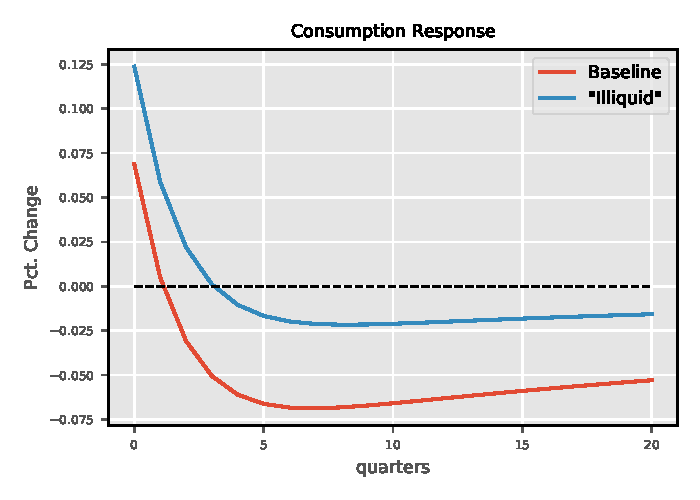
\includegraphics[width=.5\linewidth]{mainmatter/plots/SS_evaluation/Alternative_calibs/Consumption_interest_rate_response_agg_illiquid.pdf}
  }
     \caption{Responses with "illiquid" assets (reduced unhedged interest rate exposure).}
\label{fig:dC_dR_illiquid_example}
\end{figure}



\subsection{Robustness check: Household Parameters} \label{sec:C_robustness}
The responses of consumption to changes in income and the interest rate are central to the impulse responses of the model. In the standard RANK setup the household setup is sufficiently transparent such that the implication of different parameterizations are relatively easy to analyze and test. In models with heterogeneous consumers a similar robustness check is more complicated since a change in a given parameter, say, the intertemporal elasticity of substitution $\sigma$ (EIS), has two effects: 1) A different EIS affects the curvature of the Euler equation hence affecting the dynamic consumption response shape, and 2) A different EIS affect the amount of assets individuals choose to hold in steady-state, and hence the wealth distribution changes. To overcome the interplay between these two channels I do the following: To investigate the effect of the first channel I consider the change in aggregate consumption $dC$ calculated as $\sum_{i}\mathcal{D}_{i,t}^{Base}c_{i,t}$ where $\sum_{i}d\mathcal{D}_{i,t}^{Base}dc_{i,t}$ is the distribution matrix from the \textit{baseline} calibration and $dc_{i,t}$ is the change in individual consumption under the alternative parameterization. Hence I avoid distributional effects from parameter changes by fixing the distribution to the one from the baseline calibration.\footnote{keeping the distribution $\mathcal{D}$ fixed is not sufficient to match the exact same steady-state distribution since asset levels can change endogenously, but it does ensure that the distributions are very similar. Still, the marginal differences can have large effects if they change the number of constrained consumers significantly. To avoid this, I compute a reshuffling of $\mathcal{D}$ by removing a small share of consumers $\epsilon$ of the constrained consumers and adding them uniformly to all other groups with the aim being the same share of constrained consumers as in the baseline.  } \\


Figure \ref{fig:calibration_C_r_eis} shows the consumption (MPC) responses to the earlier described income and interest rate shocks (i.e. the partial equilibrium responses) for different values of the intertemporal elasticity of substitution, with $\sigma=0.5$ being the baseline value. The figure reveals that, conditional on wealth and income distributions, the dynamic consumption response is very sensitive to the choice of the EIS. Recall that a higher EIS imply less curvature in the utility of consumption, with the limiting cases $\sigma\rightarrow0,\sigma\rightarrow\infty$ corresponding to current and future consumption being perfect complements and perfect substitutes respectively. 
For the income shock a higher EIS imply that households spend more of the transitory income gain today, with the result being a higher contemporaneous MPC, and higher persistence. For the interest rate shock, the response becomes signficantly more volatile as the elasticity increases since households are more willing to substitute between current and future consumption. Neither of the EIS parametriations match the response from \citet{kaplan2018monetary}, which resembles more closely the RANK response. \\

Figure \ref{fig:calibration_C_r_std} shows the effect of varying the standard deviation of the earnings process. Note that since the standard deviation determines income dispersion it primarily affects the model through the wealth distribution, which is kept fixed here. The remaining effect from the earnings dispersion is marginal: MPCs are roughly invariant towards the dispersion, while for the interest rate shock it primarily matters for the long run persistence of the shock. The marginal differences here could, however, be due to slight changes in the wealth distribution.  \\
% Hmm this shock is proably a bit wierd???? 


\begin{figure}[H]

\centering
\begin{subfigure}{.9\textwidth}
  \centering
  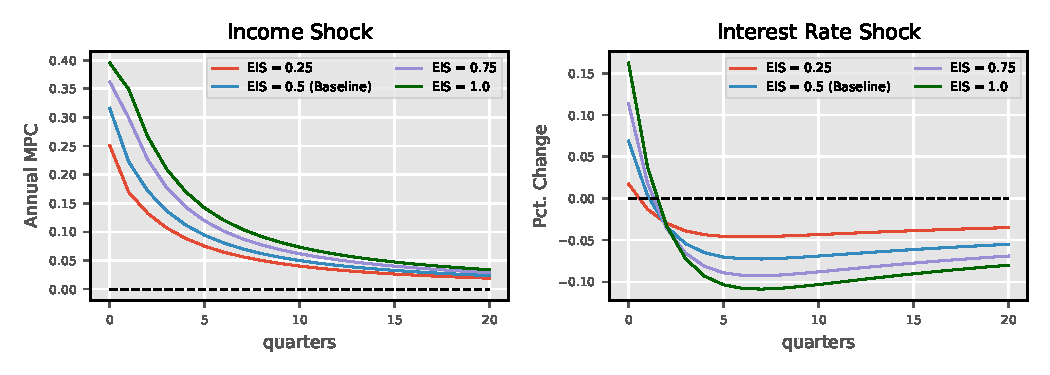
\includegraphics[width=.98\linewidth]{mainmatter/plots/SS_evaluation/Alternative_calibs/C_R_earnings_EIS.pdf} 

  \caption{Varying the intertemporal elasticity of substitution. \label{fig:calibration_C_r_eis} } 
\end{subfigure}

\begin{subfigure}{.9\textwidth}
  \centering
  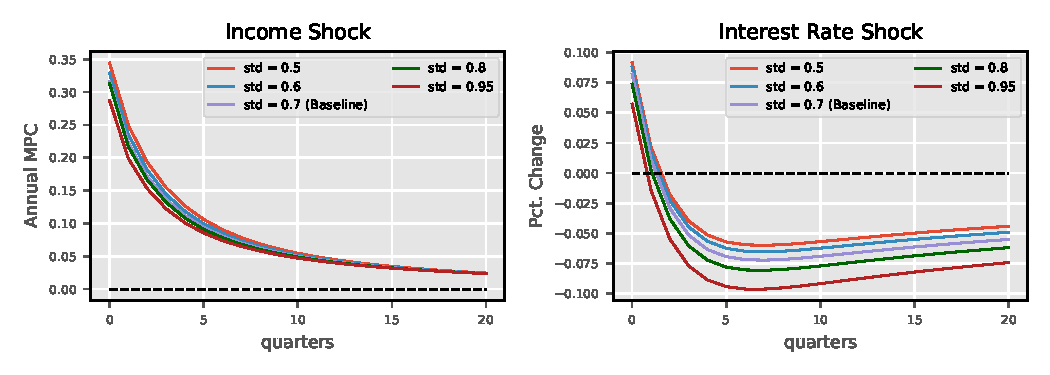
\includegraphics[width=.98\linewidth]{mainmatter/plots/SS_evaluation/Alternative_calibs/C_R_earnings_std.pdf} 
  \caption{Varying the standard deviation of earnings. }  \label{fig:calibration_C_r_std}
\end{subfigure}

\caption{Consumption responses to income and interest rate shocks under various calibrations.}
\label{fig:dC_robust}
\end{figure}


%\subsection{Reflection} % Job finding rate response. 
%I have so far considered how consumption reacts to changes in disposable income and interest rates, which are the two primarily channels that may affect consumption. Consider for a moment how each of these channels are affected by the business cycle. 

% C makes up roughly half of Y in DK 
% more volatile than GDP, but 1/3 as volatile as I. However I share of Y is 16%. 


%In typical NK models changes in disposable income are generated by changes in wages, employment, lump sum transfers and, potentially, dividends. Wages are usually considered very rigid, almost acyclical, and dividends are modeled as firm equity, not transfers. Hence it is mostly employment and lump sum transfers that can move disposable income and hence consumption. As per the exposition above, interest rates affect consumption, but probably not enough to account for the aggregate volatility observed. What remains to affect consumption decisions is essentially precautionary savings, i.e. the fact that households increase savings by cutting consumption when faced with an increase in risk. In the present model the only source of cyclical risk is through the labor market job-finding rates. 


%The remaining channel affecting consumption is not related to income or financial flows but rather behavior and expectations. In
% Add section analyzing finding rates? 


\begin{figure}[H]
\centering
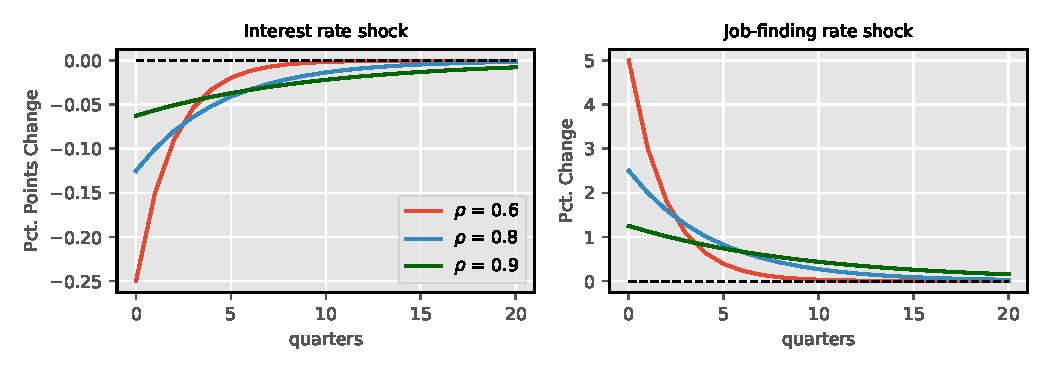
\includegraphics[width=.98\linewidth]{mainmatter/plots/C_analysis/ra_q_shocks.pdf} 
\caption{Shocks to interest- and job-finding rates with differing AR coefficient $\rho$.}
\label{fig:ra_q_shocks}
\end{figure}


\subsection{Aggregation Result: Proof} \label{Agg_result_proof}
% Assume
% no wage changes -> fixed labor suuply since no waelth effect
% borrowing constraint at zero 
% igonore  VAT - does not matter 
As in the main text I consider the aggregate change in consumption $dC_{t}=\int dc_{t}^{*}d\mathcal{D}_{ss}+\int c_{ss}^{*}d\mathcal{D}_{t}$, and specifically the term $\int dc_{t}^{*}d\mathcal{D}_{ss}$. Since we condition on the steady-state distribution of households the share of constrained households $\lambda$ is fixed. Let $c_{t}^{R}$ denote consumption of non-constrained ("Ricardian") agents and $c_{t}^{HtM}$ consumption of constrained ("Hand-to-Mouth") agents. Then:
\begin{gather*}
\int dc_{t}^{*}d\mathcal{D}_{ss}=\left(1-\lambda\right)\int dc_{t}^{R}d\mathcal{D}_{ss}^{R}+\lambda\int dc_{t}^{HtM}d\mathcal{D}_{ss}^{HtM}
\end{gather*}
The budget constraint for a constrained household is:
\begin{gather*}
c_{i,t}^{HtM}+\underline{a}=(1+r_{t}^{a})a_{i,t-1}+I_{i,t}-\tau^{I}\left(I_{i,t}\right)+T_{t}
\end{gather*}
Assume that wages are fixed and consider a first-order perturbation:
\begin{gather*}
dc_{i,t}^{HtM}=(1+r_{ss}^{a})da_{i,t-1}+\underline{a}dr_{t}^{a}+dT_{i,t}
\end{gather*}
since $a_{i,t-1}$ is fixed when conditioning on the initial distribution we have $da_{i,t-1}=0$ such that $dc_{i,t}^{HtM}=\underline{a}dr_{t}^{a}+dT_{i,t}$, which obliviously aggregates:
\begin{gather*}
\int dc_{i,t}^{HtM}d\mathcal{D}_{ss}^{HtM}=\int\underline{a}dr_{t}^{a}d\mathcal{D}_{ss}^{HtM}+\int dT_{i,t}d\mathcal{D}_{ss}^{HtM} \\
\Leftrightarrow dC_{t}^{HtM}=\underline{a}dr_{t}^{a}+dT_{t}
\end{gather*}
Rational household obey the linearized Euler equation:
\begin{gather*}
dc_{i,t}^{R}=\beta_{i}R_{ss}\left(E_{i,t}dc_{i,t+1}^{R}-\sigma R_{t+1}c_{i,ss}^{R}\right)
\end{gather*}
This disregards unemployment risk since I do not consider shock to the separation rate or the job-finding rate in this setting. Aggregating yields:
\begin{gather*}
\int dc_{i,t}^{R}d\mathcal{D}_{ss}=\int\beta_{i}R_{ss}\left(E_{i,t}dc_{i,t+1}^{R}-\sigma R_{t+1}c_{i,ss}^{R}\right)d\mathcal{D}_{ss} \\
\Leftrightarrow dC_{t}^{R}=R_{ss}\int\beta_{i}E_{i,t}dc_{i,t+1}^{R}d\mathcal{D}_{ss}-\sigma R_{t+1}C_{ss}^{R}
\end{gather*}


\subsection{Details on RA/TA household models} \label{sec:RA_TA}
\subsubsection{Canonical RA model.}
Assuming the representative family construct of \citet{merz1995search} implies that there is no idiosyncratic risk or unemployment risk. Hence only aggregate uncertainty matters, which there is none-off in the baseline model. The representative agent solves:
\begin{gather*}
V_{t}=\max_{C_{t}^{R},A_{t},\ell_{t}}\frac{C_{t}^{R}^{1-\frac{1}{\sigma}}}{1-\frac{1}{\sigma}}-\varphi\frac{\ell_{t}^{1+\frac{1}{\varphi}}}{1+\frac{1}{\varphi}}+\beta\mathbb{E}_{t}V_{t+1} \\
s.t.\\
\left(1+\tau^{c}\right)C_{t}^{R}+A_{t}=\left(1+r\right)A_{t-1}+I_{t}+T_{t}-\tau\left(I_{t}\right),
\end{gather*}
where $I_{t}=w_{t}\ell_{t}N_{t}+b_{t}\left(1-N_{t}\right)$. This results in the standard consumption Euler equation $\left(C_{t}^{R}\right)^{-\frac{1}{\sigma}}=R_{t+1}\beta\left(C_{t+1}^{R}\right)^{-\frac{1}{\sigma}}$.

\subsubsection{Canonical TA model.}
The canonical two-agent household model of \citet{campbell1989consumption} assumes that a fraction $\lambda$ of households obey a rule-of-thumb of consuming their entire income each period, and hence holds no assets. Consumption obeys:
\begin{gather*}
C_{t}^{HtM}=\frac{1}{1+\tau^{c}}\left(\lambda I_{t}-\tau\left(\lambda I_{t}\right)+\lambda T_{t}\right), \\
C_{t}=C_{t}^{R}+C_{t}^{HtM},
\end{gather*}
where $C_{t}^{R}$ is defined as above in the RA's problem, but with income flows scaled by the share of Ricardian agents $1-\lambda$.


%\subsubsection{TA model with Unemployment Risk.} 
%I assume that there is perfect insurance against idiosyncratic earnings risk but not unemployment risk. Consumption of hand-to-mouth consumers is unchanged but for Ricardian agents there now exists a representative household for employed and unemployed. Hence the model actually contains three representative agents. Consumption for the two Ricardian households obey:
%\begin{gather*}
%\left(C_{t}^{N,R}\right)^{-\frac{1}{\sigma}}=R_{t+1}\beta\left[\left(1-\delta\left(1-q_{t+1}\right)\right)\left(C_{t+1}^{N,R}\right)^{-\frac{1}{\sigma}}+\delta\left(1-q_{t+1}\right)\left(C_{t+1}^{U,R}\right)^{-\frac{1}{\sigma}}\right], \\
%\left(C_{t}^{U,R}\right)^{-\frac{1}{\sigma}}=R_{t+1}\beta\left[q_{t+1}\left(C_{t+1}^{N,R}\right)^{-\frac{1}{\sigma}}+\left(1-q_{t+1}\right)\left(C_{t+1}^{U,R}\right)^{-\frac{1}{\sigma}}\right]
%\end{gather*}
%where budget constraints associated with each state is:
%\begin{gather*}
%\left(1+\tau^{c}\right)C_{t}^{N,R}+A_{t}^{N}=\left(1+r\right)A_{t-1}^{N}+w_{t}\ell_{t}+T_{t}-\tau\left(w_{t}\ell_{t}\right), \\
%\left(1+\tau^{c}\right)C_{t}^{U,R}+A_{t}^{U}=\left(1+r\right)A_{t-1}^{U}+b_{t}+T_{t}-\tau\left(b_{t}\right)
%\end{gather*}
%Aggregate consumption for Ricardian agents is $C_{t}^{R}=N_{t}C_{t}^{N,R}+\left(1-N_{t}\right)C_{t}^{U,R}$.




\begin{figure}[H]
\makebox[\linewidth][c]{%
\centering
  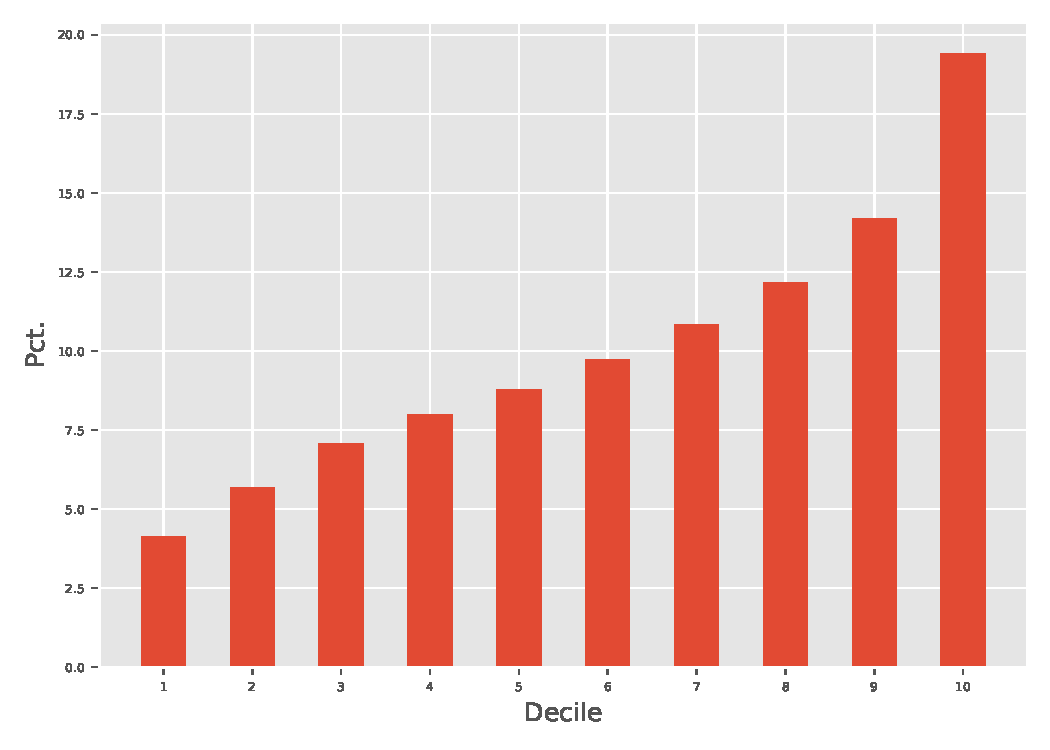
\includegraphics[width=.5\linewidth]{mainmatter/plots/SS_evaluation/C_by_deciles.pdf} 
}
\caption[Caption for LOF]{Distribution of consumption over wealth deciles in steady-state.}
\label{fig:C_dist_by_deciles}
 % {\scriptsize  Impulse responses to a negative productivity shock of 1\% with persistence 0.94 (half-life: 5 quarters). }
\end{figure}



\begin{figure}[H]
\makebox[\linewidth][c]{%
\centering
  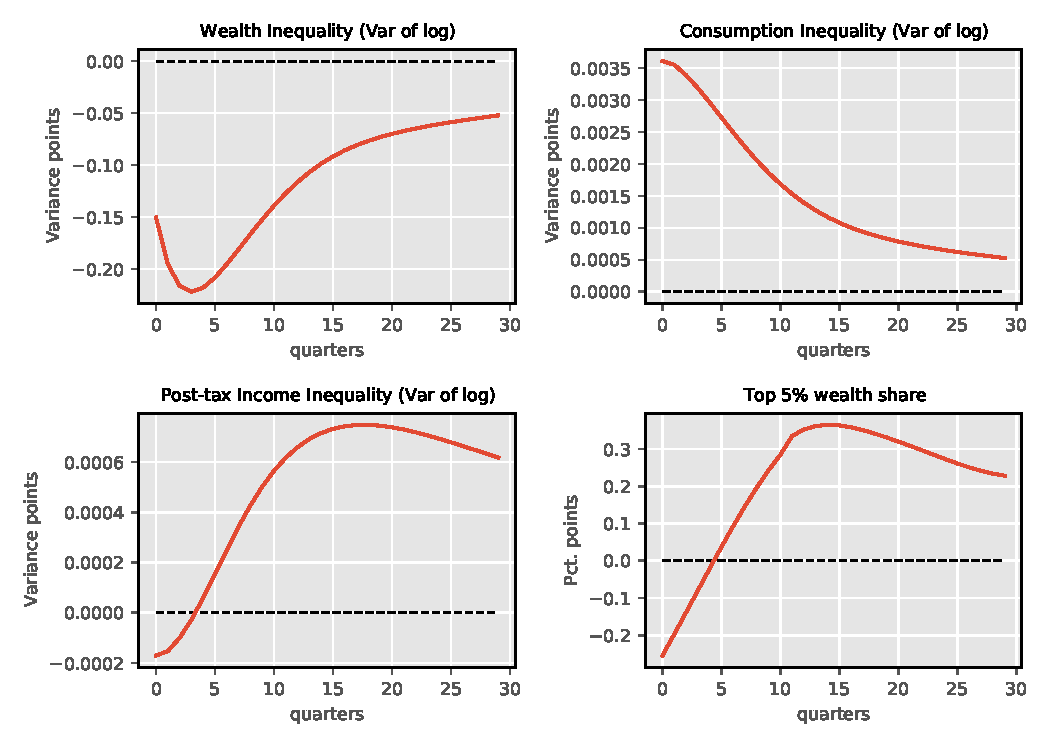
\includegraphics[width=.8\linewidth]{mainmatter/plots/SS_evaluation/TFP_shock_inequality.pdf} 
}
\caption[Caption for LOF]{Inequality responses following TFP shock.}
\label{fig:Inequality_response}
\centering
 {\scriptsize  Note: The first three panels measure wealth, consumption and income inequality over the cycle by the change in the variance of the log distribution relative to steady-state. The final panel computes the change in the wealth share of the top 5\% wealthiest households relative to steady-state.  }
\end{figure}


\section{Automatic Stabilizers- Unemployment Benefits}

\begin{figure}[H]
\makebox[\linewidth][c]{%
\centering
  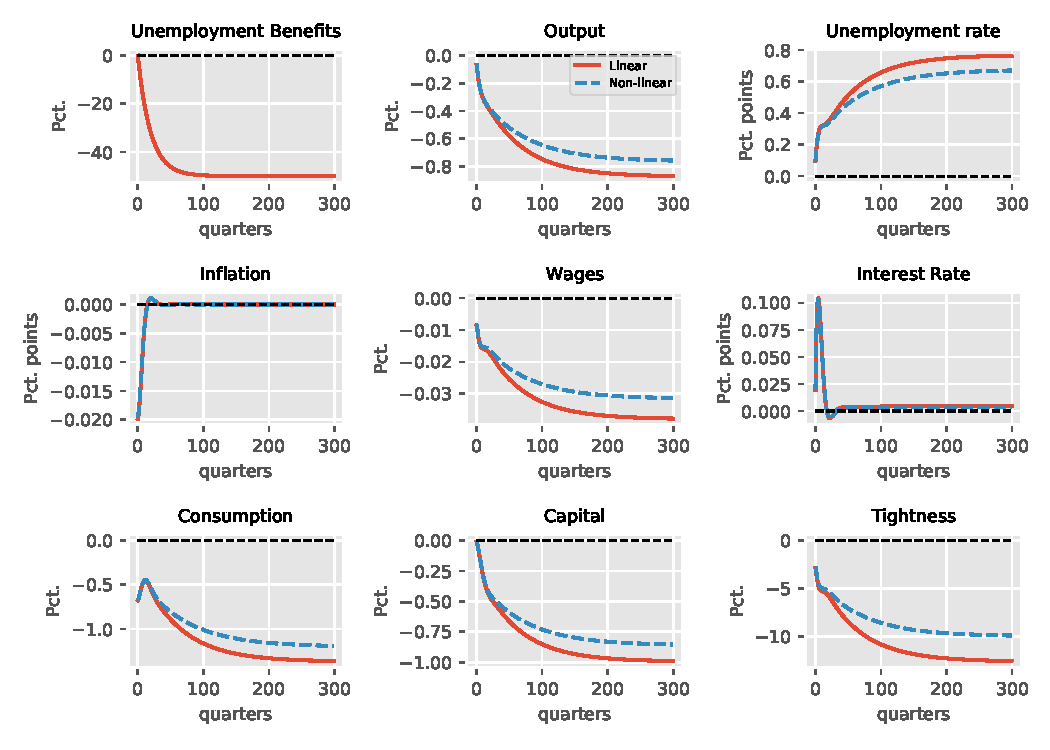
\includegraphics[width=.98\linewidth]{mainmatter/plots/Lower_b_main/transition_to_new_ss_non_linear_comp.pdf} 
}
\caption[Caption for LOF]{Transitional Dynamics following a lower unemployment benefit rate - linear and non-linear impulses.}
\label{fig:Lower_b_Transitional}
 % {\scriptsize  Impulse responses to a negative productivity shock of 1\% with persistence 0.94 (half-life: 5 quarters). }
\end{figure}



\begin{figure}[H]
\makebox[\linewidth][c]{%
\centering
  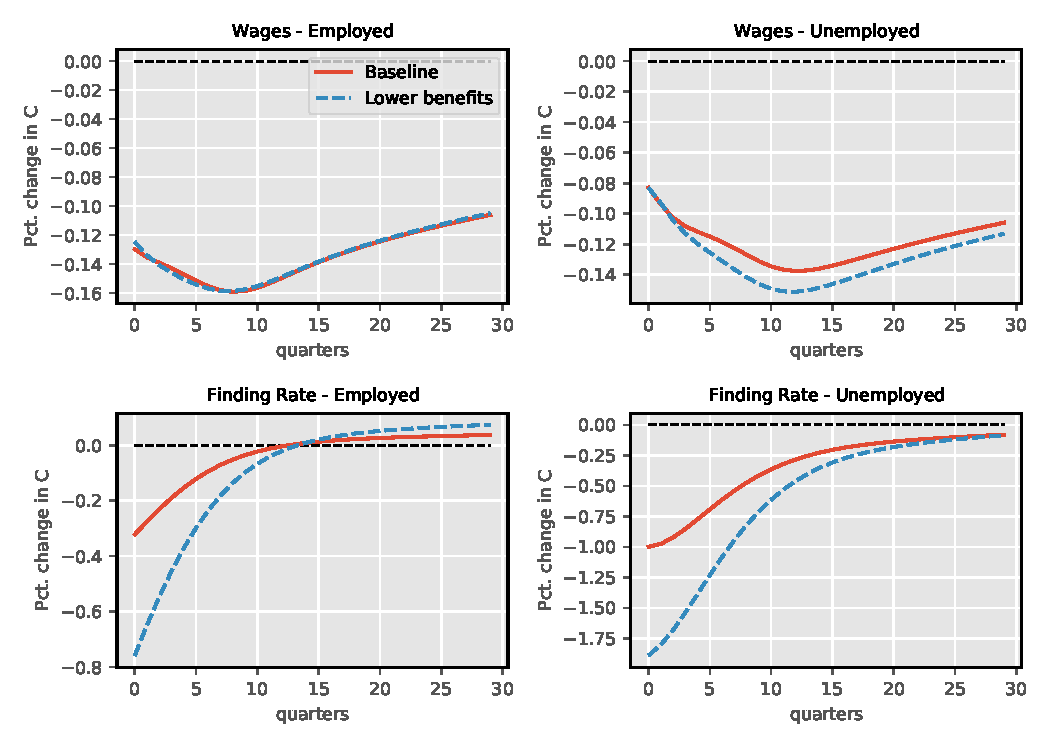
\includegraphics[width=.8\linewidth]{mainmatter/plots/Lower_b_main/main_result_C_decomp_N_U_G.pdf} 
}
\caption[Caption for LOF]{Effect on consumption from wages and job finding rate by employment status - financed by cutting government spending.}
\label{fig:lower_b_C_decomp_by_N_G}
 % {\scriptsize  Impulse responses to a negative productivity shock of 1\% with persistence 0.94 (half-life: 5 quarters). }
\end{figure}


\begin{figure}[H]
\makebox[\linewidth][c]{%
\centering
  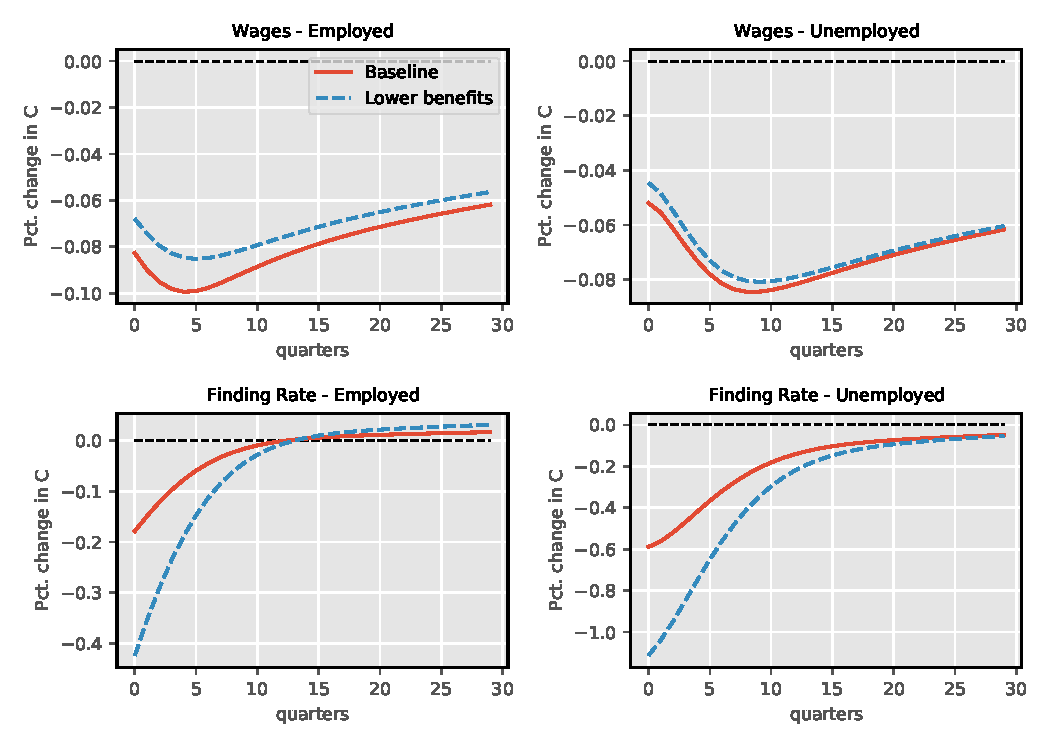
\includegraphics[width=.8\linewidth]{mainmatter/plots/Lower_b_main/main_result_C_decomp_N_U_T.pdf} 
}
\caption[Caption for LOF]{Effect on consumption from wages and job finding rate by employment status - financed by cutting transfers.}
\label{fig:lower_b_C_decomp_by_N_T}
 % {\scriptsize  Impulse responses to a negative productivity shock of 1\% with persistence 0.94 (half-life: 5 quarters). }
\end{figure}



\begin{figure}[H]
\makebox[\linewidth][c]{%
\centering
  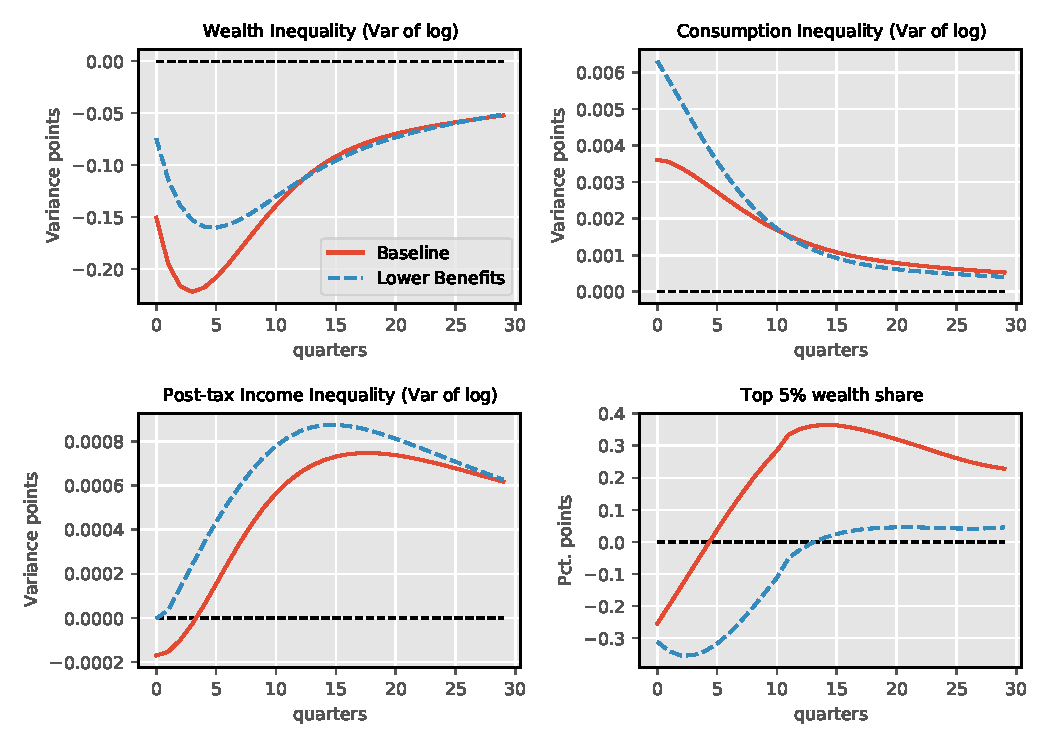
\includegraphics[width=.8\linewidth]{mainmatter/plots/Lower_b_main/agg_inequality_lower_b_G.pdf} 
}
\caption[Caption for LOF]{Inequality responses following TFP shock - comparison between baseline and model with lower unemployment benefits.}
\label{fig:Inequality_response_lower_b}
\centering
 {\scriptsize  Note: The first three panels measure wealth, consumption and income inequality over the cycle by the change in the variance of the log distribution relative to steady-state. The final panel computes the change in the wealth share of the top 5\% wealthiest households relative to steady-state.  }
\end{figure}
   % INCLUDE Discussion

\end{appendices}

% -------------------------- 
% Back matter
% --------------------------

% ********************************************************* 
% END OF THESIS
% *********************************************************
\end{document}